\chapter{Homogeneous Boltzmann equation: polar spectral scheme}
\chaptermark{HBE: polar spectral scheme}
\label{chap:boltzmann-polar}

\section{Introduction} 
\label{sect:polar-intro}

Another idea, parallel to the Fourier discretization of Chapter~\ref{chap:boltzmann-fourier} is to discretize
$f$ in two dimensions using a polar coordinate representation
\[
    f(\Bv) = \sum_{k,l} F_{k,l} \varphi_k(r) \xi_l(\theta),
\]
where the angular modes $\xi$ are ordinary complex exponentials, and the radial modes $\varphi$ are
exponentially weighted Laguerre polynomials. This has been done previously, but only for radially symmetric
solutions (i.e. no dependence on $\theta$, see for example \cite{Ender94} and \cite{Ender99}, the former
appears unavailable in English). The present work features, to the best of our knowledge, the first
development of a polar scheme for general solutions.

This method is invariably more expensive per degree of freedom than the Fourier spectral discretization, since
there is no analogue of Theorem~\ref{thm:trans-rot-Q} in the radial direction. In return, it is possible to
resolve the equilibrium solution exactly. This method will also not be affected by the aliasing that can
plague the Fourier discretization, it requires no artificial truncation, and it can be made fully conservative
for all conserved moments.

\textbf{Outline.} In Section~\ref{sec:polar} we develop the details of the polar discretization. The form of
the basis functions are motivated, and existing error estimates for stationary functions are presented (though
no attempt is made to provide time-dependent estimates). In Section~\ref{sec:polar-equilibria}, we highlight
some of the most important aspects of the method, including its expected sparsity for long times and the
conservative properties. Section~\ref{sec:polar-evaluating} explains some issues with regards to
implementation and the tricks we used to speed up the code. Finally, numerical results are presented in
Section~\ref{sec:numerical-pol} for the polar method alone, and in Section~\ref{sec:numerical-fou-pol} we
attempt to compare the Fourier and the polar methods directly.

\section{The polar Laguerre function space} \label{sec:polar}

In the following chapter we will develop a polar spectral discretization for \eqref{eqn:boltzmann-sphom}. This
method will only be developed for $d=2$, but we will point out the work required to extend it to arbitrary
dimensions where applicable.

For the sake of simplicity of notation we will identify $\bbR^2$ with $\bbC$, and its standard polar
representation,
\[
    \Bv = x(\Bv) + \ii y(\Bv) = r(\Bv) \ee^{\ii\arg\Bv}.
\]
It will also be useful to use $\mu$ to denote a specific Maxwellian, instead of more general ones as before,
\begin{equation} \label{eqn:norm-max}
    \mu(\Bv) = \mu(r) = \ee^{-r^2}.
\end{equation}

Let us now define, for $l\in\bbZ$, $k\in\bbZ_{\geq0}$, $\beta>0$
\begin{align}
    \xi_l : \quad [0,2\pi) \to \bbC \quad &: \quad \theta \mapsto \ee^{\ii l \theta}, \label{eqn:def-ce} \\
    \psi_{k,\beta}^\rmS : \quad [0,\infty) \to \bbR \quad &: 
        \quad r \mapsto \ee^{-\nicefrac{r^2}{\beta}} L_k^{(0)}(r^2), 
    \label{eqn:def-psis} \\
    \psi_{k,\beta}^\rmK : \quad [0,\infty) \to \bbR \quad &: \quad r \mapsto \frac{1}{\sqrt{k+1}}
                                                 \ee^{-\nicefrac{r^2}{\beta}} r L_k^{(1)}(r^2).
    \label{eqn:def-psik}
\end{align}
Here, $L_k^{(\alpha)}$ denote the generalized Laguerre polynomials\footnote{Often called {\em associated}
Laguerre polynomials or {\em Sonine} polynomials} of order $\alpha$. They are defined as
\begin{equation} \label{eqn:def-lag}
    L_k^{(\alpha)}(x) = \sum_{i=0}^k (-1)^k \binom{k+\alpha}{k-i} \frac{x^i}{i!},
\end{equation}
and satisfy the recurrence relations
\begin{align} 
    \label{eqn:lag0-rec} (k+1)L^{(0)}_{k+1}(x) &= (2k+1-x)L_k^{(0)}(x) - kL_{k-1}^{(0)}(x), \qquad k \geq 1, \\
    \label{eqn:lag1-rec} L_k^{(\alpha+1)}(x) &= \sum_{i=0}^k L_i^{(\alpha)}(x),
\end{align}
with $L_0^{(0)} = 1$ and $L_1^{(0)} = 1-x$. The first few polynomials of order $0$ and $1$ are tabulated in
Table~\ref{tbl:laguerre} and plotted in Figure~\ref{fig:laguerre}.

\begin{table}
\centering
\def\arraystretch{1.4}
\begin{tabular}{c@{\qquad}r@{\qquad}r}
$k$ & $L_k^{(0)}$ & $L_k^{(1)}$ \\
\hline 0 & $1$ & $1$ \\
\hline 1 & $-x+1$ & $-x+2$ \\
\hline 2 & $\frac{1}{2}x^2 - 2x + 1$ & $\frac{1}{2}x^2 - 3x + 3$ \\
\hline 3 & $-\frac{1}{6}x^3 + \frac{3}{2}x^2 - 3x + 1$ & $-\frac{1}{6}x^3 + 2x^2 - 6x + 4$ \\
\hline 4 & $\frac{1}{24}x^4-\frac{2}{3}x^3+3x^2-4x+1$ & $\frac{1}{24}x^4-\frac{5}{6}x^3+5x^2-10x+5$ \\
\end{tabular}
\caption{The first few generalized Laguerre polynomials of order $0$ and $1$.} \label{tbl:laguerre}
\end{table}

\begin{figure}
\centering
\subfloat[Order $0$]{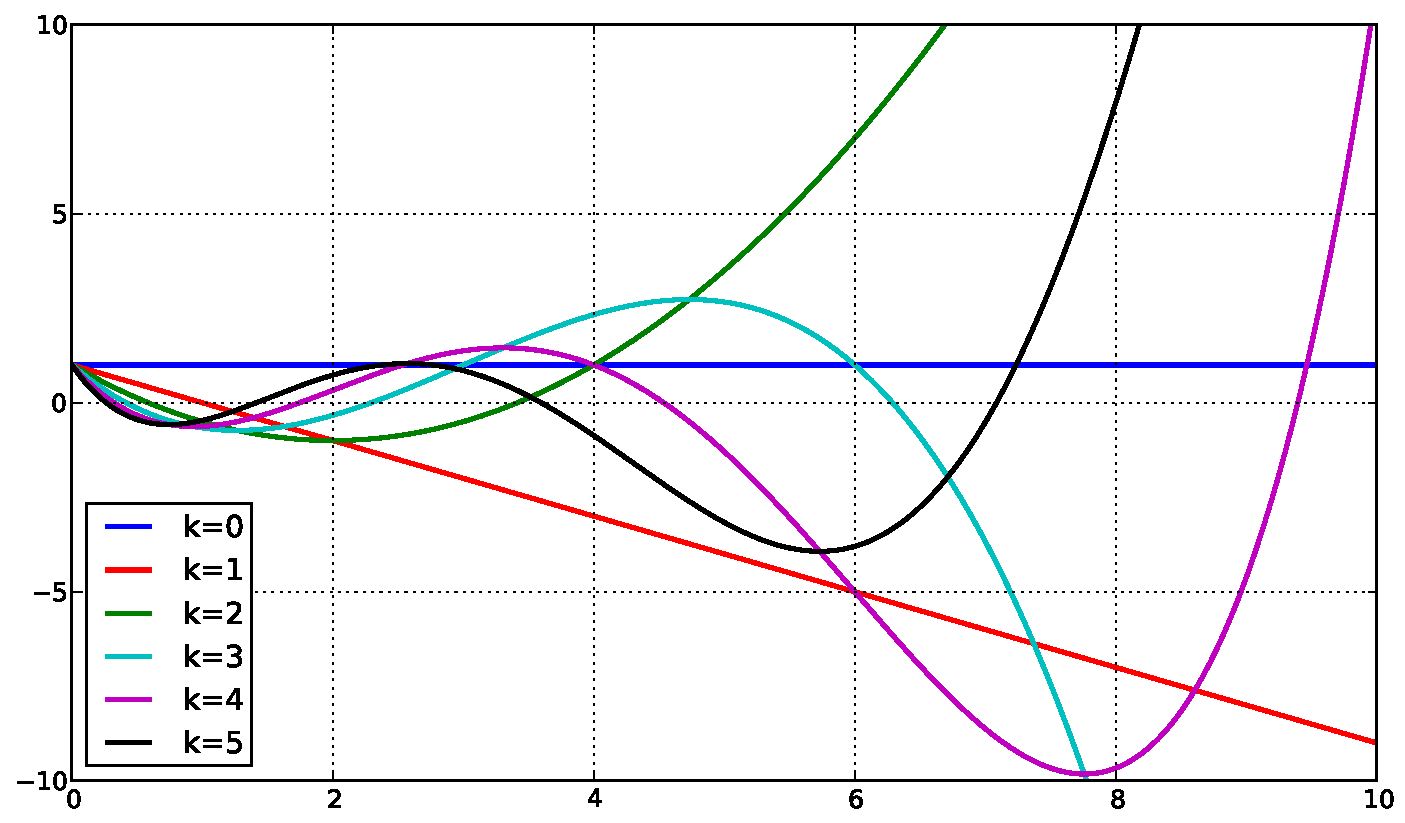
\includegraphics[width=10cm]{figs/polboltz/laguerre0}} \\
\subfloat[Order $1$]{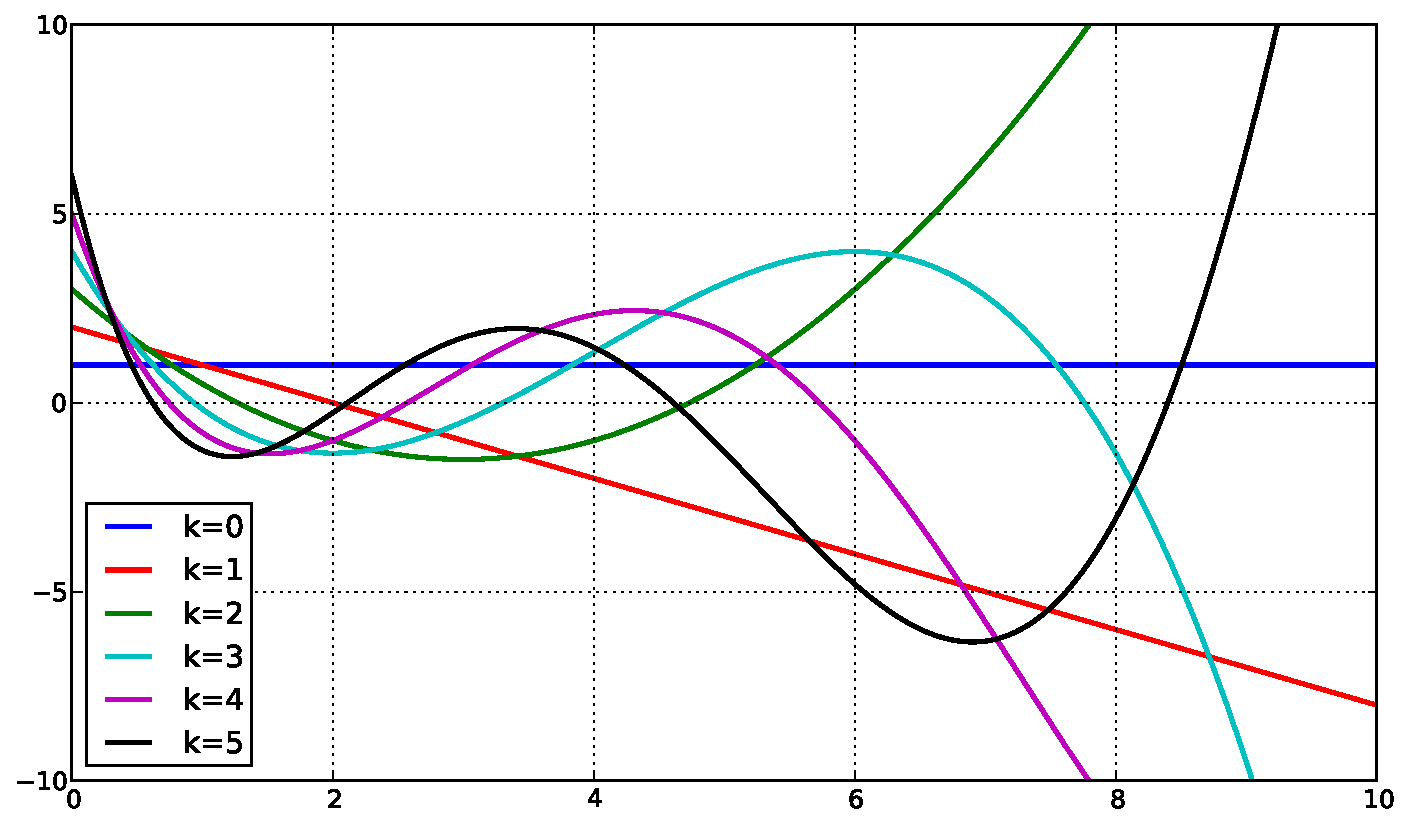
\includegraphics[width=10cm]{figs/polboltz/laguerre1}}
\caption{The first six generalized Laguerre polynomials of order $0$ and $1$.}
\label{fig:laguerre}
\end{figure}

The polynomials $L_k^{(\alpha)}$ are orthogonal with respect to the weight $\ee^{-x}x^\alpha$: 
\begin{equation} \label{eqn:lag-orth}
    \int_0^\infty \ee^{-x}x^\alpha L^{(\alpha)}_k(x) L^{(\alpha)}_l(x) \dd x 
    = \binom{k+\alpha}{k} \Gamma(\alpha + 1) \delta_{k,l}.
\end{equation}
This is the motivation for the definitions \eqref{eqn:def-psis} and \eqref{eqn:def-psik}. Substituting
$x=r^2$, we see that $\psi_{k,\beta}^{\rmS}$ and $\psi_{k,\beta}^{\rmK}$ are orthogonal with respect to the
measure
\[
    \ee^{-(1-\nicefrac{2}{\beta})r^2} r \dd r,
\]
which fits with the volume element for polar integrals over $\bbR^2$. This will be made precise in the
following.

The functions $\psi_k^\rmS$ and $\psi_k^\rmK$ from \eqref{eqn:def-psis}, \eqref{eqn:def-psik} are
exponentially weighted polynomials of degree $2k$ and $2k+1$ containing only even and odd powers of $r$,
respectively. As such, it can be expected that if $f : [0,\infty) \to \bbR$ is analytic and sufficiently rapidly
decaying (a condition depending on $\beta$), and that its analytic extension to $\bbR$ is symmetric, it will
have an exponentially convergent representation in terms of the functions $\psi_{k,\beta}^\rmS$, and likewise
for $\psi_{k,\beta}^\rmK$ if $f$ has an anti-symmetric extension to $\bbR$.

\begin{proposition} \label{prop:szasz}
Let $f:[0,\infty)\to\bbR$ be given, and assume that $f$ has a symmetric analytic extension to the
strip $s(c) \defeq \left\{ z \;:\; |\Im z| \leq \sqrt{c} \right\}$ for some $c>0$, and that for every $b$ such
that $0 \leq b<c$, there exists $C(b)$ such that
\begin{equation} \label{eqn:sz-slowdecay}
    |f(z)| \leq C(b) \exp\left[\frac{x^2}{2} - |y|\left(b^2 - y^2\right)^{\frac{1}{2}}\right],
\end{equation}
for all $z = x + \ii y \in s(b)$. Then there exist convergent Laguerre series for $f$,
\[
    f(r) = \sum_{k=0}^\infty a^{(0)}_k L_k(r^2) = \sum_{k=0}^\infty a^{(1)}_k L^{(1)}_k(r^2),
\]
where the coefficients $a^{(\alpha)}_k$ for $\alpha\in\{0,1\}$ are given by
\[
    a^{(\alpha)}_k = \frac{1}{(k+1)^\alpha}\int_0^\infty \ee^{-x} x^\alpha L^{(\alpha)}_k(x)f(\sqrt{x})\dd x
\]
and satisfy the decay property
\[
    \big|a^{(\alpha)}_k\big| \leq 2 C(b) \ee^{-2b\sqrt{k}}.
\]
\end{proposition}
\begin{proof}
The existence of the Laguerre series is given by \cite[Theorem B]{Szasz58}.  By \cite[Lemma 3.4]{Szasz58} we
also conclude that for all $b$,
\[
    \big|a^{(0)}_k\big| \leq C(b) \ee^{-2b\sqrt{k}}.
\]
The corresponding decay for $a^{(1)}_k$ holds on account of the relation $a^{(1)}_k = a^{(0)}_k -
a^{(0)}_{k+1}$, which follows from Lemma \ref{lem:adecay}.
\end{proof}
\begin{lemma} \label{lem:adecay}
The Laguerre polynomials satisfy
\[
    xL^{(1)}_k(x) = (k+1)(L^{(0)}_k(x)-L^{(0)}_{k+1}(x)).
\]
\end{lemma}
\begin{proof}
We proceed by induction. As $L_0(x)=1$ and $L_1(x)=1-x$, the statement is evidently true for $k=0$. For the
induction step, we note that
\begin{align*}
    xL^{(1)}_k 
    & \quad \overset{\mathclap{\text{\eqref{eqn:lag1-rec}}}}{=} \quad
    xL^{(1)}_{k-1} + xL^{(0)}_k \\
    & \quad \overset{\mathclap{\text{IH}}}{=} \quad
    k(L^{(0)}_{k-1} - L^{(0)}_k) + xL^{(0)}_k \\
    & \quad \overset{\mathclap{\text{\eqref{eqn:lag0-rec}}}}{=} \quad
    k(L^{(0)}_{k-1} - L^{(0)}_k) + (2k+1)L^{(0)}_k - kL^{(0)}_{k+1} - (k+1)L^{(0)}_{k+1} \\
    & \quad = \quad (k+1)(L^{(0)}_k-L^{(0)}_{k+1}).
\end{align*}
This concludes the proof.
\end{proof}

Proposition \ref{prop:szasz} establishes the necessary conditions on a function $f$ to have rapidly decaying
Laguerre series approximations in terms of $L^{(\alpha)}(r^2)$ for $\alpha\in\{0,1\}$. We now consider
expansions of symmetric and anti-symmetric functions in terms of $\psi^\rmS$ and $\psi^\rmK$.

\begin{proposition} \label{prop:sz2}
Let $f^\rmS, f^\rmK: [0,\infty) \to \bbR$ be given. Assume that $f^\rmS$ and $\frac{1}{r}f^\rmK$ have analytic
symmetric extensions to the strip $s(c)$ for some $c>0$, and that for every $b$ such that $0\leq b<c$, there
exists $C(b)$ such that 
\begin{equation} \label{eqn:sz-fastdecay}
    |f^\rmS(z)|, \left|\frac{1}{z}f^\rmK(z)\right| \leq C(b) 
    \exp\left[-\frac{|z|^2}{\beta}+\frac{x^2}{2} - |y|\left(b^2 - y^2\right)^{\frac{1}{2}}\right],
\end{equation}
for all $z=x+\ii y \in s(b)$. Then there exist convergent series
\begin{equation} \label{eqn:prop-sz2-series}
    f^\rmS(r) = \sum_{k=0}^\infty a^\rmS_{k,\beta} \psi^\rmS_{k,\beta}(r), \qquad
    f^\rmK(r) = \sum_{k=0}^\infty a^\rmK_{k,\beta} \psi^\rmK_{k,\beta}(r),
\end{equation}
where, using $\mu$ as defined in \eqref{eqn:norm-max},
\begin{equation*}
    a^\rmS_{k,\beta} = \int_0^\infty \ee^{\nicefrac{x}{\beta}-x} L_k(x) f^\rmS(\sqrt{x}) \dd x 
             = 2\int_0^\infty \mu^{1-\nicefrac{2}{\beta}}(r) \psi^\rmS_{k,\beta}(r) f^\rmS(r) r \dd r \\
\end{equation*}
and
\begin{align*}
    a^\rmK_{k,\beta} 
        &= \frac{1}{\sqrt{k+1}} \int_0^\infty \ee^{\nicefrac{x}{\beta}-x} 
                        \sqrt{x} L^{(1)}_k(x) f^\rmK(\sqrt{x}) \dd x \\
        &= 2\int_0^\infty \mu^{1-\nicefrac{2}{\beta}}(r) \psi^\rmK_{k,\beta}(r) f^\rmK(r) r \dd r,
\end{align*}
and $|a^\rmS_{k,\beta}|, |a^\rmK_{k,\beta}| \leq 2C(b)\sqrt{k+1}\;\ee^{-2b\sqrt{k}}$.
\end{proposition}
\begin{proof}
It is clear that both $f^\rmS$ and $\frac{1}{r}f^\rmK$ are even and analytic. Moreover, on account of
\eqref{eqn:sz-fastdecay}, we see that the functions
\[
    \ee^{\nicefrac{r^2}{\beta}}f^\rmS(r),\qquad \ee^{\nicefrac{r^2}{\beta}}\frac{1}{r}f^\rmK(r)
\]
both satisfy the conditions of Proposition~\ref{prop:szasz}. Thus, we have
\[
    \ee^{\nicefrac{r^2}{\beta}} f^\rmS(r) = \sum_{k=0}^\infty a^\rmS_k L_k(r^2), \qquad
    \ee^{\nicefrac{r^2}{\beta}} \frac{1}{r} f^\rmK(r) = \sum_{k=0}^\infty \tilde{a}^\rmK_k L^{(1)}_k(r^2),
\]
which gives \eqref{eqn:prop-sz2-series} with $a^\rmK_k = \tilde{a}^\rmK_k\sqrt{k+1}$. The expressions for
$a^\rmS_k$ and $a^\rmK_k$ as well as their decay follow directly from Proposition~\ref{prop:szasz}.
\end{proof}
Let us now take the step to two dimensions, and consider an analytic function $f:\bbR^2\to\bbR$. Associated
with $f$ are its symmetric and anti-symmetric parts,
\[
    f^\rmS(r,\theta) = \frac{1}{2}\left(f(r,\theta) + f(r,\theta+\pi)\right), \qquad
    f^\rmK(r,\theta) = \frac{1}{2}\left(f(r,\theta) - f(r,\theta+\pi)\right),
\]
which are also both analytic. Fixing $\theta$ (effectively considering it as a parameter), and assuming that
$f^\rmS$ and $f^\rmK$ satisfy the conditions of Proposition~\ref{prop:sz2} for some $\beta>0$, we can write
\[
    f^\rmS(r,\theta) = \sum_{k=0}^\infty a^\rmS_{k,\beta}(\theta) \psi^\rmS_{k,\beta}(r), \qquad
    f^\rmK(r,\theta) = \sum_{k=0}^\infty a^\rmK_{k,\beta}(\theta) \psi^\rmK_{k,\beta}(r),
\]
where $a^\rmS$ and $a^\rmK$ are rapidly decaying in $k$.  In fact, as $f^\rmS$ is symmetric, we should be able
to approximate $a^\rmS_{k,\beta}(\theta)$ in terms of the complex exponentials $\xi_l$ (from
\eqref{eqn:def-ce}) for {\em even} $l$, and correspondingly $a^\rmK_{k,\beta}(\theta)$ in terms of $\xi_l$ for
{\em odd} $l$.

To simplify notation, let us introduce the functions
\[
    \varphi_k^{(\beta)} = \begin{cases} 
        \psi^\rmS_{\nicefrac{k}{2},\,\beta}, & k \equiv 0\; (\Mod 2), \\ 
        \psi^\rmK_{\nicefrac{(k-1)}{2},\,\beta}, & k \equiv 1\; (\Mod 2),
    \end{cases}
\]
so that we may write
\[
    f(r,\theta) = f^\rmS(r,\theta) + f^\rmK(r,\theta) = 
    \sum_{k=0}^\infty a_k^{(\beta)}(\theta) \varphi_k^{(\beta)}(r),
\]
where $a_k$ corresponds to $a^\rmS_{\nicefrac{k}{2},\,\beta}$ for even $k$ and to
$a^\rmK_{\nicefrac{(k-1)}{2},\,\beta}$ for odd $k$, and where $a_k$ has the same parity as $k$, i.e.
$a_k(\theta+\pi) = (-1)^k a_k(\theta)$.

Continuing from before, we now write
\[
    a_k^{(\beta)}(\theta) = \sum_{2\,|(k-l)} F_{k,l}^{(\beta)} \xi_l(\theta),
\]
where
\[
    F_{k,l}^{(\beta)} = \frac{1}{2\pi} \int_0^{2\pi} a_k^{(\beta)}(\theta) \xi_{-l}(\theta) \dd\theta.
\]
Let us first consider $k$ even. Then
\begin{align*}
    F_{k,l}^{(\beta)} &= \frac{1}{\pi} \int_0^{2\pi} \int_0^\infty \mu^{1-\nicefrac{2}{\beta}}
             \varphi_k^{(\beta)} \xi_{-l} f^\rmS \; r \dd r \dd\theta \\
          &= \frac{1}{\pi} \int_{\bbR^2} \mu^{1-\nicefrac{2}{\beta}} \varphi_k^{(\beta)} 
             \xi_{-l} f^\rmS \dd \Bv
           = \frac{1}{\pi} \int_{\bbR^2} \mu^{1-\nicefrac{2}{\beta}} \varphi_k^{(\beta)} 
             \xi_{-l} f \dd \Bv,
\end{align*}
since $\xi_{-l}$ is even, the corresponding integral with $f^\rmK$ will be zero. Precisely the same argument
applies for $k$ odd. As such, we arrive at
\begin{equation} \label{eqn:polexp}
    f(r,\theta) = \sum_{2\,|(k-l)} F_{k,l}^{(\beta)} \; \varphi_k^{(\beta)} (r) \xi_l(\theta),
\end{equation}
where the notation $a|b$ is understood to mean that $a$ divides evenly into $b$. The coefficients are given by
\[
    F_{k,l}^{(\beta)} = \frac{1}{\pi} \int_{\bbR^2} \mu^{1-\nicefrac{2}{\beta}} 
                        \varphi_k^{(\beta)} \xi_{-l} f \dd\Bv.
\]
This implies that the functions $\varphi_k^{(\beta)}\xi_l$ form an orthogonal system with respect to the
weight $\mu^{1-\nicefrac{2}{\beta}}$. This is in fact the case, and it is not difficult to see.
\begin{proposition} \label{prop:orthopol}
Assuming $k_1 \equiv l_1\;(\Mod2)$ and $k_2\equiv l_2\;(\Mod2)$, we have
\[
    \left\langle \varphi_{k_1}^{(\beta)} \xi_{l_1}, \varphi_{k_2}^{(\beta)} \xi_{l_2} 
    \right\rangle_{L^2(\bbR^2;\,\beta)} 
    = \int_{\bbR^2} \mu^{1-\nicefrac{2}{\beta}} 
      \varphi_{k_1}^{(\beta)} \xi_{l_1} \varphi_{k_2}^{(\beta)} \xi_{-l_2} \dd\Bv
    = \pi \delta_{k_1,k_2} \delta_{l_2,l_2}.
\]
\end{proposition}
\begin{proof}
First, we note that if $k_1$ and $k_2$ have different parities, the integrand in question is odd, so the
integral is zero. Thus, we assume from now that they have equal parities. We have
\begin{align*}
    \left\langle \varphi^{(\beta)}_{k_1}\xi_{l_1}, \varphi^{(\beta)}_{k_2}\xi_{l_2} 
    \right\rangle_{L^2(\bbR^2;\,\beta)} 
    &= \int_0^{2\pi} \xi_{l_1-l_2} \dd\theta \int_0^\infty \mu^{1-\nicefrac{2}{\beta}}
       \varphi_{k_1}^{(\beta)} \varphi_{k_2}^{(\beta)}\; r \dd r \\
    &= 2\pi\delta_{l_1,l_2} \int_0^\infty \mu^{1-\nicefrac{2}{\beta}}
       \varphi_{k_1}^{(\beta)} \varphi_{k_2}^{(\beta)} \;r \dd r. \\
\end{align*}
For $k_1, k_2$ both even, we have
\begin{align*}
    \int_0^\infty \mu^{1-\nicefrac{2}{\beta}} \varphi_{k_1}^{(\beta)} \varphi_{k_2}^{(\beta)} r \dd r
    &= \int_0^\infty \ee^{-r^2} L_{\nicefrac{k_1}{2}}(r^2) L_{\nicefrac{k_2}{2}}(r^2)\; r \dd r \\
    &= \frac{1}{2} \int_0^\infty \ee^{-x} L_{\nicefrac{k_1}{2}}(x) L_{\nicefrac{k_2}{2}}(x) \dd x
    \overset{\text{\eqref{eqn:lag-orth}}}{=} \frac{1}{2} \delta_{k_1,k_2}.
\end{align*}
And for $k_1, k_2$ both odd, we find, using $Z(a,b)=[(a+1)(b+1)]^{-\nicefrac{1}{2}}$,
\begin{align*}
    \int_0^\infty \mu^{1-\nicefrac{2}{\beta}} \varphi_{k_1}^{(\beta)} \varphi_{k_2}^{(\beta)} r \dd r
    &= 2Z(k_1,k_2) \int_0^\infty
       \ee^{-r^2} r^2 L^{(1)}_{\nicefrac{(k_1-1)}{2}}(r^2) L^{(1)}_{\nicefrac{(k_2-1)}{2}}(r^2)\; r \dd r \\
    &= Z(k_1,k_2) \int_0^\infty 
       \ee^{-x} x L^{(1)}_{\nicefrac{(k_1-1)}{2}}(x) L^{(1)}_{\nicefrac{(k_2-1)}{2}}(x) \dd x \\
    & \overset{\text{\eqref{eqn:lag-orth}}}{=} \frac{1}{2} \delta_{k_1,k_2}.
\end{align*}
This concludes the proof.
\end{proof}
We will use the notation $L^2(\bbR^2;\,\beta)$ to denote the weighted space in which the orthogonality holds,
with inner product
\[
    \langle f,g \rangle_{L^2(\bbR^2;\,\beta)} = \int_{\bbR^2} \mu^{1-\nicefrac{2}{\beta}} f g \dd\Bv.
\]
We also note in passing that $L^2(\bbR^2;\,2)=L^2(\bbR^2)$, that is, for $\beta=2$ we have orthogonality with
respect to the usual Lebesgue measure.

Thus, for $K,L,\beta>0$ and $L$ even, we define the finite-dimensional function spaces
\[ \boxed{
    \cV_\beta(K,L) = \spann \left\{ \varphi^{(\beta)}_k\xi_l \;:\; 0\leq k < K, \; -L \leq l < L, \;
    k \equiv l \;(\Mod 2) \right\}
} \]
of dimension $KL$, and we denote the implied basis by $\cB_\beta(K,L)$. The requirement that $L$ is even is
made purely for simplifying reasons, as the basis functions can then be enumerated as $b_{k,q} = \varphi_k
\xi_{l(q,k)}$ for $0 \leq k < K$ and $0 \leq q < L$, where
\begin{equation} \label{eqn:pol-enum}
    l(q,k) = \begin{cases} 2q - (-1)^k,& q < \nicefrac{L}{2} \\
                           2(q-L) - (-1)^k,& \text{otherwise}.
             \end{cases}
\end{equation}
Let us also denote by $P_{\cV_\beta(K,L)}$ (or, when convenient, merely $P_\cV$) the
$L^2(\bbR^2;\,\beta)$-orthogonal projection onto $\cV_\beta(K,L)$. Then, given an initial condition
$f_0(\Bv)$, we propose to solve \eqref{eqn:boltzmann-sphom} approximately through the projected equation
\[
    \frac{\partial f_\cV}{\partial t} = P_\cV Q(f_\cV,f_\cV), \qquad
    f_\cV(0) = P_\cV f_0.
\]
It is noteworthy that, unlike \eqref{eqn:boltzmann-nd}, there is no need to truncate the collision operator in
this case. In this way we also avoid all the aliasing effects which plague the Fourier methods.

\section{Equilibria and initial values}
\label{sec:polar-equilibria}

The space $\cV_\beta(K,L)$ contains functions on the form 
\[
    \varphi^{(\beta)}_0\xi_0 = \exp(-\nicefrac{|\Bv|^2}{\beta}),
\]
which are equilibrium solutions with mass density $\beta\pi$, momentum $\Bzero$ and temperature
$\nicefrac{\beta}{2}$. Thus, if the initial condition conforms to these conditions, we can expect that for
$k,l$ not both zero, the corresponding coefficient $F^{(\beta)}_{k,l}$ tends to zero.  If the initial
condition does not conform, the equilibrium solution cannot be exactly represented in any finite space
$\cV_\beta(K,L)$, but owing to the equilibrium solution being isotropic (if $\Bu=\Bzero$), it will certainly
still have a sparse representation. In this case, we expect $F^{(\beta)}_{k,l}$ to tend to zero for all
$l\neq0$.

\begin{definition} \label{def:conf}
    We say that a function $f(\Bv)$ is $\beta$-{\em conforming} if
    \[
        \rho(f) = \beta\pi, \qquad
        \Bu(f) = \Bzero, \qquad
        T(f) = \frac{\beta}{2}.
    \]
\end{definition}

\begin{theorem} \label{thm:trf-sols}
    Let $g(t,\Bv)$ be a solution to \eqref{eqn:boltzmann-sphom}, where $B$ satisfies Assumption~\ref{ass:B}.
    Let $\alpha,\gamma > 0$ be given, and define $\eta = \nicefrac{\alpha}{\gamma^{\lambda+2}}$. Then
    \[
        h(t,\Bv) = \alpha g(\eta t, \gamma \Bv)
    \]
    is also a solution to \eqref{eqn:boltzmann-sphom}.
\end{theorem}
\begin{proof}
    First,
    \begin{align*}
        \frac{\partial h}{\partial t}(t,\Bv)
        &= \alpha\eta \frac{\partial g}{\partial t}(\eta t, \gamma \Bv) \\
        &= \alpha\eta \int_{\bbR^2}\int_{\bbS^1} |\gamma\Bv-\overline{\Bv}_\ast|^\lambda b(\cos\theta) \\
        & \qquad\qquad\qquad\qquad
            \left[ g(\eta t,\overline{\Bv}') g(\eta t,\overline{\Bv}_\ast') -
                   g(\eta t,\gamma\Bv) g(\eta t,\overline{\Bv}_\ast) \right]
            \dd\Bsigma \dd\overline{\Bv}_\ast,
    \end{align*}
    where the collision identities read
    \[
        \overline{\Bv}', \overline{\Bv}_\ast' = \frac{1}{2}\left(
        \gamma\Bv+\overline{\Bv}_\ast \pm |\gamma\Bv-\overline{\Bv}_\ast|\Bsigma \right).
    \]
    Making the change of variables $\overline{\Bv}_\ast, \overline{\Bv}', \overline{\Bv}_\ast'
    = \gamma\Bv_\ast, \gamma\Bv', \gamma\Bv_\ast'$, we recover the familiar collision identity
    \[
        \Bv', \Bv_\ast' = \frac{1}{2}\left(
        \Bv+\Bv_\ast \pm |\Bv-\Bv_\ast|\Bsigma \right),
    \]
    whence
    \begin{align*}
        \frac{\partial h}{\partial t}(t,\Bv)
        &= \alpha\eta \int_{\bbR^2}\int_{\bbS^1} |\gamma\Bv-\gamma\Bv_\ast|^\lambda b(\cos\theta) \\
        & \qquad\qquad\qquad
            \left[ g(\eta t,\gamma\Bv) g(\eta t,\gamma\Bv_\ast') -
                   g(\eta t,\gamma\Bv) g(\eta t,\gamma\Bv_\ast) \right]
            \dd\Bsigma \dd(\gamma\Bv_\ast) \\
        &= \frac{\eta\gamma^{\lambda+2}}{\alpha} Q(h,h)(\Bv).
    \end{align*}
    Since $\nicefrac{\eta\gamma^{\lambda+2}}{\alpha}=1$, this concludes the proof.
\end{proof}
\begin{remark}
    A corresponding result to Theorem~\ref{thm:trf-sols} holds in arbitrary dimensions $d$, where
    $\eta=\nicefrac{\alpha}{\gamma^{\lambda+d}}$.
\end{remark}
The ``problem'' of nonconforming initial values is easily overcome. Theorem~\ref{thm:trf-sols} allows us to
transform any initial condition $f(0,\Bv)$ to conform to the space $\cV_\beta(K,L)$, solve it there, and then
recover the solution later, as demonstrated in the following theorem. This is important to the viability of
the method, since conformity can be maintained without assembling discrete collision operators for a variety
of different spaces with different values of observables.
\begin{theorem} \label{thm:conf-sols}
    Let $f(t,\Bv)$ be a solution to \eqref{eqn:boltzmann-sphom}, where $B$ satisfies Assumption~\ref{ass:B}.
    Let $\beta>0$ be given, and assume $f$ has mass density, momentum and temperature $\rho$, $\Bu$ and $T$. 
    Define
    \begin{equation} \label{eqn:poltrf}
        \gamma = \sqrt{\frac{2T}{\beta}}, \qquad
        \alpha = \frac{2\pi T}{\rho}, \qquad
        \eta   = \frac{\alpha}{\gamma^{\lambda+2}}.
    \end{equation}
    Then 
    \[
        h(t,\Bv)=\alpha f(\eta t, \gamma\Bv + \Bu)
    \]
    is a conforming solution to \eqref{eqn:boltzmann-sphom}, and $f$ can be recovered via $f(t,\Bv) =
    \alpha^{-1} h(\nicefrac{t}{\eta}, \nicefrac{(\Bv-\Bu)}{\gamma})$.
\end{theorem}
\begin{proof}
    We show that $h$ is conforming. Indeed,
    \begin{equation} \label{eqn:poltrf-mass}
        \rho(h) = \alpha\int_{\bbR^2} f(\gamma\Bv+\Bu) \dd\Bv 
        = \frac{\alpha}{\gamma^2}\int_{\bbR^2} f(\gamma\Bv+\Bu) \dd(\gamma\Bv+\Bu)
        = \frac{\alpha}{\gamma^2}\rho,
    \end{equation}
    and
    \begin{align}
        \nonumber T(h) &= \frac{1}{2\rho(h)} \int_{\bbR^2} \alpha f(\gamma\Bv+\Bu) \dd\Bv
        = \frac{1}{2\gamma^2\rho}\int_{\bbR^2} f(\Bs)|\Bs-\Bu|^2\dd\Bs \\
        \nonumber &= \frac{1}{2\gamma^2\rho}\left[ \int_{\bbR^2}f(\Bs)|\Bs|^2\dd\Bs +
           |\Bu|^2\int_{\bbR^2}f(\Bs)\dd\Bs - 2\Bu\cdot\int_{\bbR^2}f(\Bs)\Bs\dd\Bs\right] \\
        &= \frac{1}{2\gamma^2}\left[E + |\Bu|^2 - 2|\Bu|^2\right] = \frac{1}{\gamma^2}T.
        \label{eqn:poltrf-T}
    \end{align}
    Setting $\rho(h)=\beta\pi$ and $T(h)=\nicefrac{\beta}{2}$, and solving
    \eqref{eqn:poltrf-mass}-\eqref{eqn:poltrf-T} for $\alpha,\gamma$, we find precisely \eqref{eqn:poltrf}. It
    is easy to see that $\Bu(h)=\Bzero$. 
    
    It being a solution to \eqref{eqn:boltzmann-sphom} is an easy corollary of theorems \ref{thm:trans-rot-Q}
    and \ref{thm:trf-sols}.
\end{proof}

\subsection{Choice of $\beta$}

The properties of the bases $\cB_\beta$ depend rather heavily on the value of $\beta$. We have already noted
that for $\beta=2$, the weighted inner product $\langle\cdot,\cdot\rangle_{L^2(\bbR^2;\,\beta)}$ becomes the
usual $L^2$ inner product, and so error analysis in familiar norms will be simpler. In fact, one observes
that for most functions $f$, the coefficients $F_{k,l}^{(\beta)}(f)$ decay fastest for $\beta=2$, and one can
consistently achieve better error rates than $\beta<2$, both in the weighted norm and the $L^2$-norm.

On the other hand, we have the following Theorem concerning the stability of the bases with respect to the
observables.
\begin{theorem} \label{thm:polobs}
Let $\beta>0$ be given and define the linear functionals\footnote{Here we have abused notation somewhat, since
the quantity $(E\rho)(f)$ as defined is only equal to $E(f)\rho(f)$ if $\rho(f)\neq0$, and similarly for
$\Bu\rho$.}
\begin{gather*}
    \rho(f) = \int_{\bbR^2} f(\Bv) \dd\Bv, \qquad
    (\Bu \rho)(f) = \int_{\bbR^2} f(\Bv) \Bv \dd\Bv,\\
    (E \rho)(f) = \int_{\bbR^2} f(\Bv) |\Bv|^2 \dd\Bv.
\end{gather*}
Then,
\begin{align*}
    \rho\left(\xi_0\psi^\rmS_{k,\beta}\right) &= \beta\pi(1-\beta)^k, \\
    (\Bu\rho)\left(\xi_{\pm 1}\psi^\rmK_{k,\beta}\right) &= \frac{\beta^2\pi}{2}\sqrt{k+1}(1-\beta)^k
    \begin{pmatrix}1\\\pm1\end{pmatrix}, \\
    (E\rho)\left(\xi_0\psi^\rmS_{k,\beta}\right) &= 
        \begin{cases}
            \beta^2\pi[1-(k+1)\beta](1-\beta)^{k-1}, & k>0, \\
            \beta^2\pi, & k=0,
        \end{cases}
\end{align*}
using the convention that $0^0=1$ if $\beta=1$. For all other valid combinations of $\xi_l$ and
$\psi^\cdot_{k,\beta}$ the functionals evaluate to zero.
\end{theorem}
\begin{proof}
The proof for this is not difficult, but it involves a fair amount of algebra. First, we have the expansion of
Laguerre polynomials in terms of monomials,
\[
    L_k^{(\alpha)}(x) = \sum_{i=0}^k \binom{k+\alpha}{k-i} \frac{(-1)^i}{i!} x^i.
\]
For mass density and temperature, we first note that any integration against $\xi_l$ for $l\neq0$ must yield
zero. For momentum, note that (considering $\Bv$ as a complex number) we have $\Bv = \xi_1(\Bv) r$, so any
integration against $\xi_l$ for $l\neq-1$ must yield zero.

Thus, for mass density we have
\begin{align*}
\rho\left(\xi_0\psi^\rmS_{k,\beta}\right) 
&= 2\pi \int_0^\infty \ee^{-\nicefrac{r^2}{\beta}} L_k(r^2) \,r \dd r
 = \beta\pi \int_0^\infty \ee^{-u} L_k(\beta u) \dd u \\
&= \beta\pi \int_0^\infty \ee^{-u} \sum_{i=0}^k \binom{k}{i} \frac{(-1)^i}{i!} (\beta u)^i \dd u \\
&= \beta\pi \sum_{i=0}^k \binom{k}{i} \frac{(-\beta)^i}{i!} 
   \underbrace{\int_0^\infty \ee^{-u} u^i \dd u}_{=\Gamma(i+1)=i!} \\
&= \beta\pi \sum_{i=0}^k \binom{k}{i} (-\beta)^i 1^{k-i}
 = \beta\pi(1-\beta)^k.
\end{align*}
For energy the technique is mostly the same, except one needs the identity $\binom{k}{i} = \frac{k}{i}
\binom{k-1}{i-1}$ for $k,i>0$. Thus, for $k>0$ we find
\begin{align*}
(E\rho)\left(\xi_0\psi^\rmS_{k,\beta}\right)
&= 2\pi \int_0^\infty \ee^{-\nicefrac{r^2}{\beta}} r^2 L_k(r^2) \, r \dd r
 = \beta^2\pi \int_0^\infty \ee^{-u} u L_k(\beta u) \dd u \\
&= \beta^2\pi \int_0^\infty \ee^{-u} u \sum_{i=0}^k \binom{k}{i} \frac{(-1)^i}{i!} (\beta u)^i \dd u \\
&= \beta^2\pi \sum_{i=0}^k \binom{k}{i} \frac{(-\beta)^i}{i!} \int_0^\infty \ee^{-u} u^{i+1} \dd u \\
&= \beta^2\pi \sum_{i=0}^k \binom{k}{i} (i+1) (-\beta)^i \\ \displaybreak
&= \beta^2\pi \underbrace{\sum_{i=0}^k \binom{k}{i}(-\beta)^i}_{=(1-\beta)^k}
   + \beta^2\pi \sum_{i=1}^k \underbrace{\binom{k}{i}i}_{=k\binom{k-1}{i-1}}(-\beta)^i \\
&= \beta^2\pi \left[ (1-\beta)^k - \beta k \sum_{i=1}^k \binom{k-1}{i-1} (-\beta)^{i-1} \right] \\
&= \beta^2\pi \left[ (1-\beta)^k - \beta k (1-\beta)^{k-1} \right]
 = \beta^2\pi [1-(k+1)\beta](1-\beta)^{k-1}.
\end{align*}
If $k=0$ the second sum falls away, and one is left with $\beta^2\pi$.

Lastly, momentum:
\begin{align*}
(\Bu\rho)\left(\xi_{\pm1}\psi^\rmK_{k,\beta}\right)
&= \int_0^{2\pi} \ee^{\pm\ii\theta} \begin{pmatrix} \cos\theta \\ \sin\theta \end{pmatrix} \dd\theta
   \int_0^\infty \ee^{-\nicefrac{r^2}{\beta}} r^2 L_k^{(1)}(r^2) \, r \dd r \\
&= \frac{\beta^2\pi}{2}\begin{pmatrix}1\\\pm1\end{pmatrix}
   \int_0^\infty \ee^{-u} u L_k^{(1)}(\beta u) \dd u \\
&= \frac{\beta^2\pi}{2}\begin{pmatrix}1\\\pm1\end{pmatrix} 
   \int_0^\infty \ee^{-u} u \sum_{i=0}^k \binom{k+1}{k-i} (\beta u)^i \dd u \\
&= \frac{\beta^2\pi}{2}\begin{pmatrix}1\\\pm1\end{pmatrix}
   \sum_{i=0}^k \binom{k+1}{k-i} \frac{(-\beta)^i}{i!} \int_0^\infty \ee^{-u} u^{i+1} \dd u \\
&= \frac{\beta^2\pi}{2}\begin{pmatrix}1\\\pm1\end{pmatrix}
   \sum_{i=0}^k \underbrace{\binom{k+1}{k-i}(i+1)}_{=(k+1)\binom{k}{i}} (-\beta)^i \\
&= \frac{\beta^2\pi}{2}\begin{pmatrix}1\\\pm1\end{pmatrix} (k+1) \sum_{i=0}^k \binom{k}{i} (-\beta)^i \\
&= \frac{\beta^2\pi}{2}\begin{pmatrix}1\\\pm1\end{pmatrix} (k+1)(1-\beta)^k,
\end{align*}
where we have suppressed the factor $(k+1)^{-\nicefrac{1}{2}}$.
\end{proof}
In particular, we note the following asymptotic rates.
\begin{corollary} \label{cor:polobs}
It holds that
\begin{itemize}
\item for $0<\beta<2$ we have exponential decay of observables for basis functions as $k\to\infty$, i.e.
\[
    \rho\left(\psi^\rmS_{k,\beta}\right) = (\Bu\rho)\left(\xi_{\pm1}\psi^\rmK_{k,\beta}\right)
    = (E\rho)\left(\psi^\rmS_{k,\beta}\right) = \cO(|\beta-1|^k).
\]
All these bases are stable with respect to observables.
\item for $\beta=1$ we have exactness,
\begin{gather*}
    \rho\left(\psi^\rmS_{k,1}\right) = \delta_{0,k}\pi, \qquad
    (\Bu\rho)(\xi_{\pm1}\psi^\rmK{k,1}) = \delta_{0,k} \pi \begin{pmatrix}1\\\pm1\end{pmatrix},\\
    (E\rho)\left(\psi^\rmS_{k,1}\right) = \begin{cases} \pi,&k=0,\\ -\pi,&k=1,\\ 0,&k\geq2. \end{cases}
\end{gather*}
\item for $\beta=2$ we have polynomial instability,
\[
    \rho\left(\psi^\rmS_{k,\beta}\right) \in \cO(1), \qquad
    (\Bu\rho)\left(\xi_{\pm1}\psi^\rmK_{k,\beta}\right) \in \cO(\sqrt{k}), \qquad
    (E\rho)\left(\psi^\rmS_{k,\beta}\right) \in \cO(k).
\]
\item for $\beta>2$ we have exponential instability,
\[
    \rho\left(\psi^\rmS_{k,\beta}\right) = (\Bu\rho)\left(\xi_{\pm1}\psi^\rmK_{k,\beta}\right)
    = (E\rho)\left(\psi^\rmS_{k,\beta}\right) = \cO((\beta-1)^k).
\]
\end{itemize}
\end{corollary}
From this point of view, $\beta=1$ is optimal, as it can promise exact conservation of {\bf all} conserved
observables.

The last detail to keep in mind is that any $\beta>2$ results in an unbounded basis, that is
\[
    \sup_k \; \sup_r \left|\varphi^{(\beta)}_k(r)\right| = \infty.
\]
This fact follows from the following asymptotic expression \cite[Equation 2.12]{Gavrilyuk11}:
\[
    L_k^{(\alpha)}(x) = \pi^{-\nicefrac{1}{2}} \ee^{\nicefrac{x}{2}}
                        x^{-\nicefrac{\alpha}{2}-\nicefrac{1}{4}}
                        k^{\nicefrac{\alpha}{2}-\nicefrac{1}{4}}
                        \left[ \cos\left(2\sqrt{kx}-\omega\pi\right) + 
                               \cO\left(k^{-\nicefrac{1}{2}}\right)
                        \right],
\]
for some $\omega$ depending on $\alpha$, but not on $x$ or $k$.

In summary, $\beta=2$ will offer somewhat faster norm convergence and easy analysis in the $L^2$-norm, while
$\beta=1$ guarantees exact conservation of all observables. One might also employ a value $1<\beta<2$ as a
compromise, while the condition $\beta \leq 2$ ought to be considered absolute.

In this dissertation we have only performed experiments with $\beta\in\{1,2\}$. No other values will be
jonsidered here.

\section{Evaluating collisions}
\label{sec:polar-evaluating}

We now turn to the practical aspects of evaluating $Q(f,g)$ for $f,g\in \cV_\beta(K,L)$. Taking the
$L^2(\bbR^2;\,\beta)$-orthogonal approximation by discarding the extra coefficients, we have
\begin{equation} \label{eqn:polar-update}
    Q(f,g) = \sum_{k,l}\left(\sum_{k_1,k_2,l_1,l_2} 
             S_{k_1,k_2,l_1,l_2}^{k,l} F^{(\beta)}_{k_1,l_1} G^{(\beta)}_{k_2,l_2} \right)
             \varphi^{(\beta)}_k\xi_l,
\end{equation}
where $F^{(\beta)}_{k,l}, G^{(\beta)}_{k,l}$ are the coefficients for $f$ and $g$ respectively (according to
\eqref{eqn:polexp}), and
\[
    S_{k_1,k_2,l_1,l_2}^{k,l} = \frac{1}{\pi} \left\langle Q\left(\varphi^{(\beta)}_{k_1} \xi_{l_1},
    \varphi^{(\beta)}_{k_2} \xi_{l_2}\right), \varphi^{(\beta)}_k \xi_l \right\rangle_{L^2(\bbR^2;\,\beta)}.
\]
Of course, the entries of the tensor $S$ also depend on $\beta$, but we have suppressed this. $S$ is
$K^3L^3$-dimensional, and forming a sum such as \eqref{eqn:polar-update} at each timestep is extremely
expensive. However, there are some mitigating factors. In particular, the following corollary of Theorem
\ref{thm:trans-rot-Q}.
\begin{corollary} \label{cor:rot-Q}
Let $f$ and $g$ be of the form
\[
    f(r,\theta) = f_r(r) \ee^{\ii k \theta}, \qquad g(r,\theta) = g_r(r) \ee^{\ii l \theta},
\]
for some $f_r$, $g_r$, $k$ and $l$. Then,
\[
    Q(f,g)(r,\theta) = C(r) \ee^{\ii (k+l) \theta}
\]
for some function $C$ depending on $f_r$, $g_r$, $k$ and $l$.
\end{corollary}
\begin{proof}
Let $\rho_\omega$ be a rotation operator through $\omega$, that is
\[
    \rho_\omega f(r,\theta) = f(r,\theta-\omega)
\]
We get $\rho_\omega f = \ee^{-\ii k \omega} f$, and correspondingly for $g$. Using Theorem
\ref{thm:trans-rot-Q} and the bilinearity of $Q$ we the obtain
\[
    \rho_\omega Q(f,g)(r,\theta) = \ee^{-\ii (k+l) \omega} Q(f,g)(r,\theta).
\]
Choose $\omega=\theta$ and rearrange to find
\[
    Q(f,g)(r,\theta) = \ee^{\ii (k+l) \theta} \rho_\theta Q(f,g)(r,\theta).
\]
The result follows since $\rho_\theta Q(f,g)(r,\theta) = Q(f,g)(r,0)$ is independent of $\theta$.
\end{proof}
By Corollary~\ref{cor:rot-Q}, $S$ is nonzero only for $l_1+l_2=l$, reducing the complexity to $K^3L^2$.
Assuming $K=L=N$ degrees of freedom in each direction, and generalizing to arbitrary dimensions, this yields a
complexity of ``only'' $N^{2d+1}$ compared to the $N^{2d}$ of the Fourier spectral discretization.
\begin{remark} \label{rem:rot-pol}
The core problem with generalizing this method to higher dimensions is to find an analogue of
Corollary~\ref{cor:rot-Q} for $d>2$. The problem of rotating expansions in spherical harmonics is nontrivial.
The classical text is \cite{Wigner31}. For more recent work, see for example \cite{Ivanic96} (real spherical
harmonics) and \cite{Lessig12}.

At least, what can be said is that these rotation operators are band-restricted, so that a rotated spherical
harmonic $Y_l^m$ contains no contributions from harmonics with degrees different from $l$.
\end{remark}

Among other factors, we note that adaptive timestepping methods, reducing the dimension of the numerical
solution space, ought to be particularly effective in this method, since the solution will converge to a
member of the basis for any initial condition (and conformity can be enforced by Theorem~\ref{thm:conf-sols}.
Moreover, the computation of $S$ and the timestepping itself is particularly open to parallelization.

\subsection{Computing the discrete collision operator}

Let us now turn to the issue of evaluating the coefficients of $K$. For this, we will split the operator into
gain and loss parts, and first consider the loss part.
\begin{align*}
    S_{k_1,k_2,l_1,l_2}^{k,l\;(-)} 
    &= \frac{1}{\pi} \left\langle Q^-\left(\varphi^{(\beta)}_{k_1} \xi_{l_1},
    \varphi^{(\beta)}_{k_2} \xi_{l_2}\right), \varphi^{(\beta)}_k \xi_l \right\rangle_{L^2(\bbR^2;\,\beta)} \\
    &= \frac{1}{\pi} \int_{\bbR^2}\int_{\bbR^2}\int_{\bbS^1}B(|\Bv-\Bv_\ast|,\cos\theta) \\
    & \qquad\qquad\qquad
    \left(\mu^{1-\nicefrac{2}{\beta}}\varphi^{(\beta)}_{k_1}\xi_{l_1} \varphi^{(\beta)}_{k}\xi_{-l}\right)(\Bv)
    \left(\varphi^{(\beta)}_{k_2}\xi_{l_2}\right)(\Bv_\ast)
    \dd\Bsigma\dd\Bv_\ast\dd\Bv \\
    &= \frac{1}{\pi}
    \int_{\bbR^2} \left(\mu^{1-\nicefrac{2}{\beta}} 
            \varphi^{(\beta)}_{k_1}\xi_{l_1} \varphi^{(\beta)}_{k}\xi_{-l}\right)(\Bv)
    \int_{\bbR^2} \left(\varphi^{(\beta)}_{k_2}\xi_{l_2}\right)(\Bv_\ast) \cI^-(\Bv,\Bv_\ast) \dd\Bv_\ast \dd\Bv,
\end{align*}
where the {\em inner integral} $\cI^-$ is given by
\[
    \cI^-(\Bv,\Bv_\ast) = \int_{\bbS^1} B(|\Bv-\Bv_\ast|, \cos\theta) \dd\Bsigma
\]
and prevents us from separating the two integrals over $\bbR^2$. It is generally not the case that $\cI^-$ is
low rank (i.e. it is expressible as a small sum of decomposable terms $a_1(\Bv)a_2(\Bv_\ast)$), so such a
strategy of simplification may be misguided. However, it {\em is} a function of just one real variable, namely
$|\Bv-\Bv_\ast|$, so in the context of quadrature, it does not have to be evaluated very many times. In
fact, by Assumption~\ref{ass:B}, we have
\[
    \cI^-(\Bv,\Bv_\ast) = |\Bv-\Bv_\ast|^\lambda \int_{\bbS^1} b(\cos\theta) \dd\Bsigma.
\]
For the Maxwellian kernel, $B\equiv\nicefrac{1}{2\pi}$, the loss part is particularly easy to evaluate, as
$\cI^-\equiv1$, giving
\begin{align*}
    S_{k_1,k_2,l_1,l_2}^{k,l\;(-)} 
    &= \frac{1}{\pi} \int_{\bbR^2} \left( \mu^{1-\nicefrac{2}{\beta}}
       \varphi^{(\beta)}_{k_1}\xi_{l_1} \varphi^{(\beta)}_{k}\xi_{-l}\right)\dd\Bv
       \int_{\bbR^2} \left(\varphi^{(\beta)}_{k_2}\xi_{l_2}\right)\dd\Bv_\ast \\
    &= \frac{1}{\pi} \left\langle\varphi^{(\beta)}_{k_1}\xi_{l_1}, 
                                 \varphi^{(\beta)}_{k}\xi_{l}\right\rangle_{L^2(\bbR^2;\,\beta)} 
       \rho\left(\varphi^{(\beta)}_{k_2}\xi_{l_2}\right) \\
       &= \delta_{k,k_1}\;\delta_{l,l_1}\;\delta_{0,l_2}\;\rho\left(\varphi^{(\beta)}_{k_2}\right)
\end{align*}
Theorem~\ref{thm:polobs} provides the mass densities.

Let us now turn to the gain part. In a similar vein as before, we find
\begin{align*}
    S_{k_1,k_2,l_1,l_2}^{k,l\;(+)} 
    &= \frac{1}{\pi} \left\langle Q^+\left(\varphi^{(\beta)}_{k_1} \xi_{l_1},
    \varphi^{(\beta)}_{k_2} \xi_{l_2}\right), \varphi^{(\beta)}_k \xi_l \right\rangle_{L^2(\bbR^2;\,\beta)} \\
    &= \frac{1}{\pi} \int_{\bbR^2}\int_{\bbR^2}\int_{\bbS^1}B(|\Bv-\Bv_\ast|,\cos\theta)
    \left(\varphi^{(\beta)}_{k_1}\xi_{l_1}\right)(\Bv')
    \left(\varphi^{(\beta)}_{k_2}\xi_{l_2}\right)(\Bv_\ast') \\
    & \qquad\qquad\qquad\qquad
    \left(\mu^{1-\nicefrac{2}{\beta}}\varphi^{(\beta)}_{k}\xi_{-l}\right)(\Bv)
    \dd\Bsigma\dd\Bv_\ast\dd\Bv \\
    &= \frac{1}{\pi}
    \int_{\bbR^2} \left(\varphi^{(\beta)}_{k_1}\xi_{l_1}\right)(\Bv)
    \int_{\bbR^2} \left(\varphi^{(\beta)}_{k_2}\xi_{l_2}\right)(\Bv_\ast)
    \cI_{k,l}^+(\Bv,\Bv_\ast)\dd\Bv_\ast\dd\Bv
\end{align*}
with
\begin{equation} \label{eqn:inner-trf-before}
    \cI_{k,l}^+(\Bv,\Bv_\ast) = \int_{\bbS^1} B(|\Bv-\Bv_\ast|, \cos\theta) 
    \left(\mu^{1-\nicefrac{2}{\beta}}\varphi_{k}\xi_{-l}\right)(\Bv') \dd\Bsigma.
\end{equation}
Here, we have made a change of variables $\Bv,\Bv_\ast \longleftrightarrow \Bv',\Bv_\ast'$, revealing a
striking similarity with the loss term. However, in this case we find the $(k,l)$-dependence in the inner
integral, which makes the gain term somewhat more challenging, even for simple cases like the Maxwellian
kernel.

In analyzing $\cI^+$ it will be helpful to consider $\Bv,\Bv_\ast$ as complex numbers. (Note, however, that
while the integrals are complex-valued, they are not complex integrals.) In the following, let us also make
the simplifying assumption of considering only constant $b(\cos\theta)\equiv b$, known as the Variable Hard
Spheres (VHS) assumption.

After making the substitution $\Bv'=e^{\ii\arg(\Bv+\Bv_\ast)}\Bw'$, we find
\begin{equation} \label{eqn:trf-inner}
    \cI_{k,l}^+(\Bv,\Bv_\ast) = |\Bv-\Bv_\ast|^\lambda b\;\xi_{-l}(\arg(\Bv+\Bv_\ast))\int_{\bbS^1}
    \left(\mu^{1-\nicefrac{2}{\beta}}\varphi^{(\beta)}_k\xi_l\right)(\Bw')\dd\Bsigma,
\end{equation}
where now $\Bw'$ runs over a circle centered at $\nicefrac{1}{2}|\Bv+\Bv_\ast|$ with radius
$\nicefrac{1}{2}|\Bv-\Bv_\ast|$ (see Figure~\ref{fig:inner-trf}). In particular, the integral in
\eqref{eqn:trf-inner} is real, and depends only on the two real quantities $|\Bv+\Bv_\ast|$ and
$|\Bv-\Bv_\ast|$ (and not on their arguments).  Additionally, $\cI^+$ depends on the argument of
$\Bv+\Bv_\ast$, but this dependence is trivial and requires no quadrature to track.

\begin{figure}
    \centering
    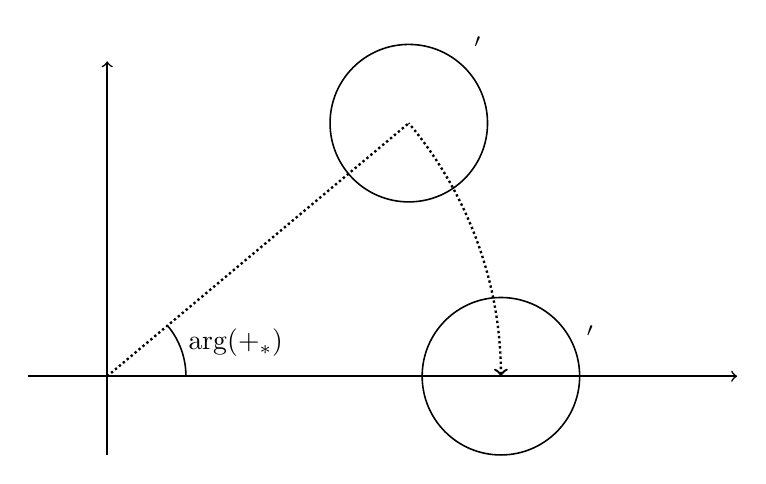
\begin{tikzpicture}
        \coordinate[label={[label distance=1cm]45:$\Bv'$}] (before) at (40:5);
        \coordinate[label={[label distance=1cm]15:$\Bw'$}] (after) at (0:5);
        \coordinate[label={0:$\arg(\Bv+\Bv_\ast)$}] (angle) at (25:1);
        \draw[densely dotted, <-, line width=0.03cm] (0:5) arc (0:40:5);
        \draw[line width=0.02cm] (0:1) arc (0:40:1);
        \draw[densely dotted, line width=0.03cm] (0,0) -- (before);
        \draw[line width=0.02cm, ->] (-1,0) -- (8,0);
        \draw[line width=0.02cm, ->] (0,-1) -- (0,4);
        \draw[line width=0.02cm] (before) circle (1);
        \draw[line width=0.02cm] (after) circle (1);
    \end{tikzpicture}
    \caption{Transforming the integral $\cI^+$ from \eqref{eqn:inner-trf-before} to \eqref{eqn:trf-inner}.}
    \label{fig:inner-trf}
\end{figure}

\subsection{Adaptivity} \label{sec:pol-adapt}

To aid the expensive timestepping calculations, and to take advantage of the expected exponential decay of all
coefficients $F_{k,l}$ except $k=l=0$, we have implemented a simple adaptive scheme reducing the
number of degrees of freedom when coefficients reach a threshold value.

As we will see in the numerical experiments, coefficients go to zero in an order which is primarily determined
by $l$. That is, in general, $F_{k_1,l_1}$ will reach a threshold value before $F_{k_2,l_2}$ if $|l_1|>|l_2|$.

This suggests the following simple adaptivity check: after every timestep, check the magnitude of the
coefficients $F_{k,l}$ with $l\in\{-L,\,-L+1,\,L-1,\,L-2\}$. If they are all below the threshold, reduce $L$
by $2$.

We consider no adaptivity in the other direction, i.e. for increasing the solution space. From numerical
observations of the time-dependent behaviour of the solution coefficients, they will almost always decay.

\subsection{Spatial inhomogeneity} \label{sec:pol-inhom}

Some of the listed advantages of the polar method over the Fourier discretization depend on the fact that the
solution will converge to a function that lies in the solution space (in the conforming case), or if not, is
isotropic and thus has a sparse representation. These conditions might fail to hold in the solution of a
spatially {\em in}homogeneous Boltzmann equation, where the equilibrium solution might depend on the spatial
variable $\Bx$ under certain source terms and boundary conditions. In this case, conformity can no longer be
guaranteed at every point, nor can isotropy of the equilibrium be taken for granted (say, if the global
momentum in the system is nonzero).

We have not performed experiments with the spatially inhomogeneous Boltzmann equation in this work. However,
we have performed limited experiments in the homogeneous case where conformity and equilibrium isotropy are
deliberately discarded. These results are discussed in Section~\ref{sec:nonconf}. The results indicate that
the method might still be viable in this case, and that adaptivity might still be useful, although solutions
computed using $\beta=2$ should be considered dubious.

\section{Numerical results} \label{sec:numerical-pol}

Throughout this section, all quadrature in $\Bv$ has been performed using a polar tensor product quadrature
rule with Gauss-Laguerre in the radial direction and the trapezoidal rule in the angular direction. For the
computation of the collision tensor $S$, we used $61$-point quadrature in both directions (this includes
$61$-point trapezoidal quadrature for the inner integrals $\cI^-$ and $\cI^+$). For evaluation of the initial
condition and errors, we used the same quadrature rule.

Timestepping was performed using the same fourth order Runge-Kutta rule as in Section~\ref{sec:numerical-fou},
using a timestep of $10^{-2}$ for $\beta=1$ and $5\cdot10^{-3}$ for $\beta=2$, to compensate for the fact that
time runs twice as quickly in the latter case. As for the Fourier discretization, stiffness does not
seem to be a problem.

\subsection{Verification (BKW)} \label{sec:numpol-verify}

Precisely as in Section~\vref{sec:verify}, we use the BKW solution to verify the correctness of the polar
discretization scheme. Let $f$ be defined as in \eqref{eqn:bkw}, and write
\begin{equation} \label{eqn:pol-bkw}
    g(t,\Bv) = 2\pi f(2\pi t, \Bv).
\end{equation}
Then $g$ is a $2$-conforming solution to \eqref{eqn:boltzmann-sphom}, and $g(\nicefrac{t}{2},\sqrt{2}\Bv)$ is
the corresponding $1$-conforming solution.

The $L^2$-errors for this test are shown, depending on $t$, $K$ and $\beta$, in Figure~\vref{fig:numpol-bkw}.
One can observe exponential convergence to zero both in $K$ and $t$, as expected. No dependence on $L$ is
shown, since $g$ is isotropic for all times.

We observe that the error decays exponentially to a threshold level for all $K$. This threshold is mostly due
to quadrature error, and not timestepping. The $\beta=2$ method is better for solutions far removed from
equilibrium, but $\beta=1$ eventually achieves better accuracy.

One may compare to Figure~\vref{fig:bkw} (showing the same experiment for the Fourier method), but this is of
limited usefulness since the Polar scheme is naturally fitted to the BKW solution, it being radially symmetric
and having a sparse representation.

\begin{figure}
\centering
\subfloat[$L^2$-error versus time.]{
    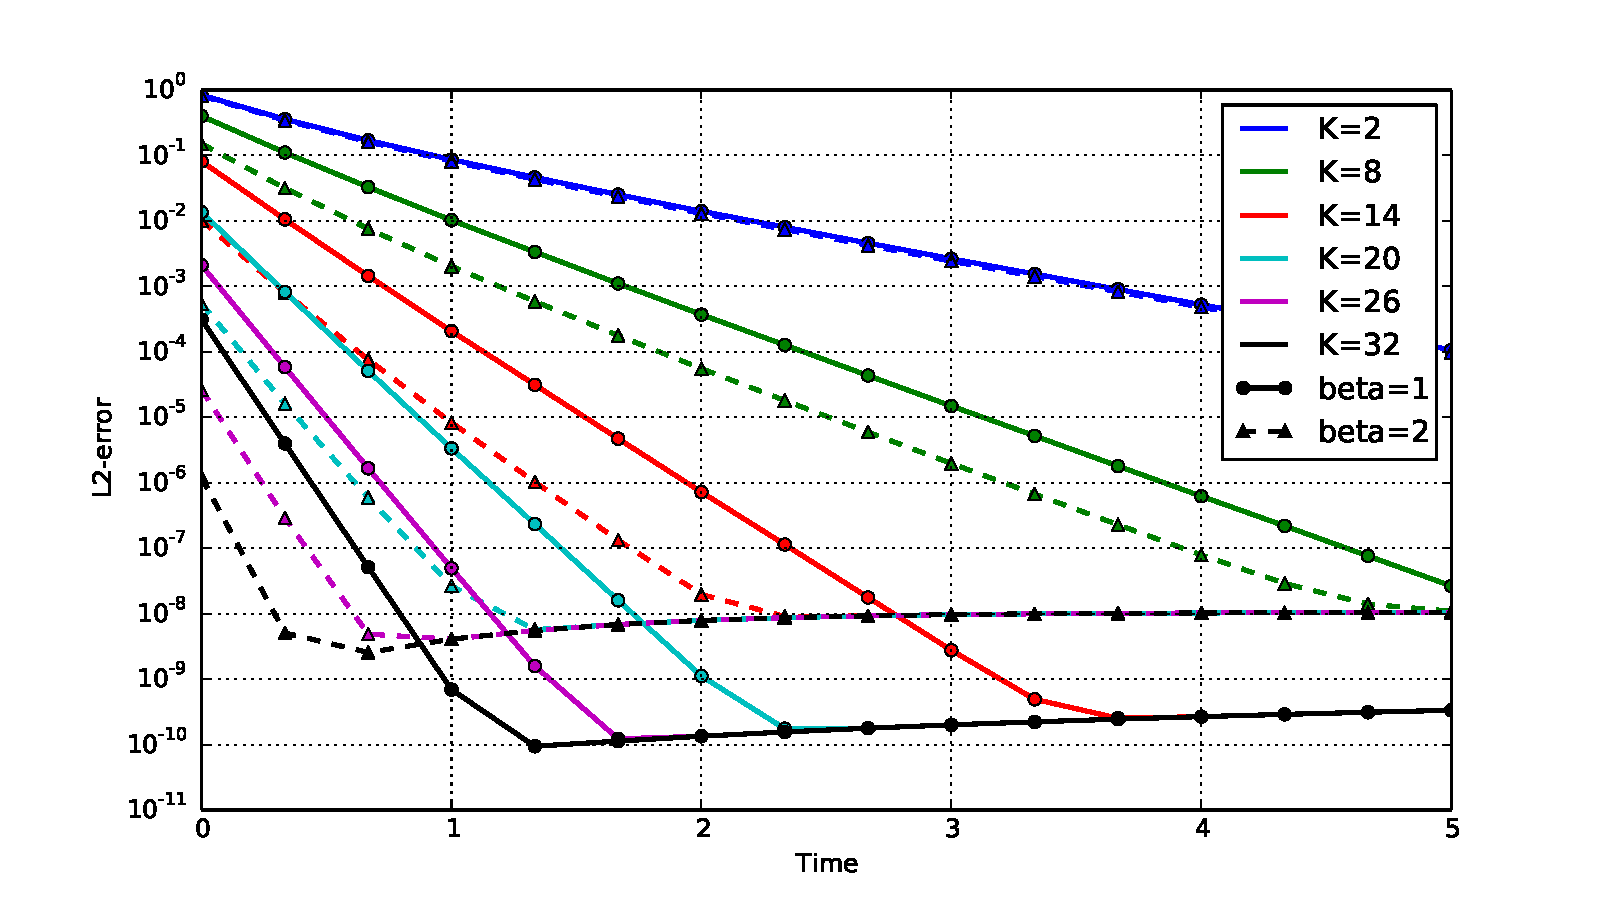
\includegraphics[width=14cm]{figs/polboltz/bkw}
} \\
\subfloat[$L^2$-error versus $K$.]{
    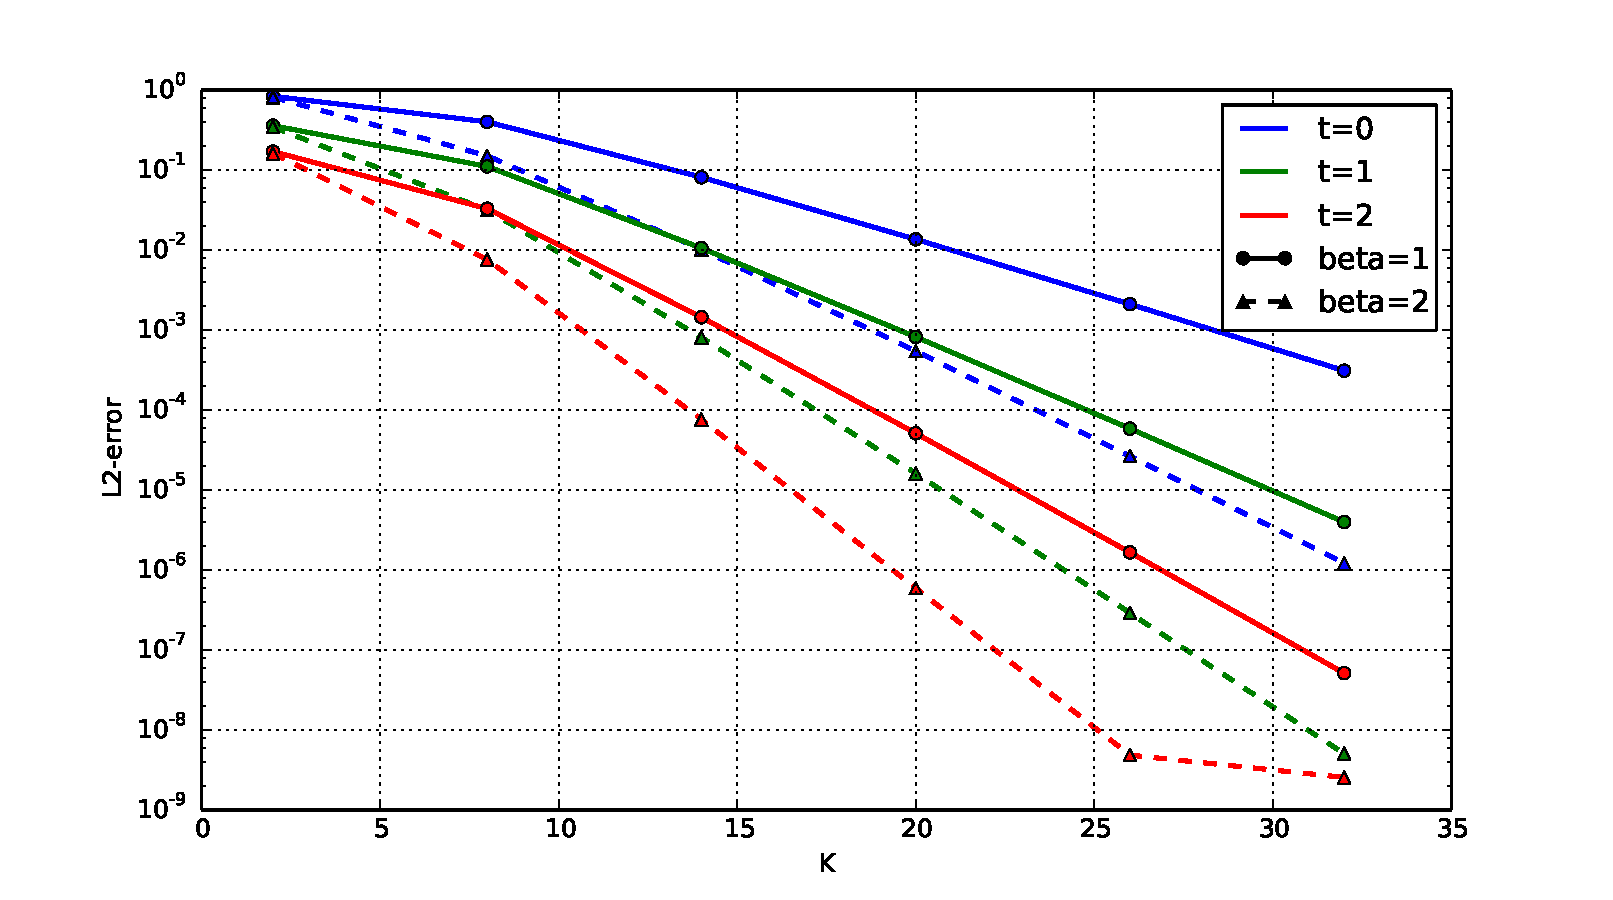
\includegraphics[width=14cm]{figs/polboltz/bkw-flip}
}
\caption{$L^2$-error for the BKW solution depending on $K$ and time. See Section~\vref{sec:numpol-verify} for
details.}
\label{fig:numpol-bkw}
\end{figure}

\subsection{Crossed streams} \label{sec:numpol-cb}

Given constants $R,S>0$, a $2$-conforming crossed streams initial condition can be constructed as follows:
\begin{align*}
    \eta(c,v,w) &= \exp\left[-g(S(v-c)^2 + (w-c)^2)\right] \\
    f_0(\Bv) &= \alpha\left( \eta(c,v_x,v_y) + \eta(-c,v_y,v_x) \right)
\end{align*}
with
\[
    \delta = 4R^2+\frac{1}{S}+1, \qquad
    \alpha = \frac{\delta}{4}\sqrt{S}, \qquad
    g = \frac{\delta}{4}, \qquad
    c = \frac{R}{\sqrt{g}}.
\]
Here, $R$ regulates the relative velocity between the two streams, and $S$ the relative spread of the two
streams in each direction (parallel and perpendicular to the momentum).

Figure~\vref{fig:numpol-cb} shows some samples of approximate solutions to this initial condition with $S=3$,
$R=1$, with a relatively large number of degrees of freedom.

Figure~\vref{fig:numpol-cb-obs} shows the error in observables as a function of time for both values of
$\beta$. As expected, $\beta=1$ is considerably more accurate than $\beta=2$. The experiment also shows a
slight unexpected worsening of the energy and momentum for $\beta=1$, which should be constant. This can
likely be attributed to quadrature error.

Figure~\vref{fig:numpol-cb-ent} shows the entropy of the numerical solution as a function of time for $K=44$,
$L=26$, and may be compared to Figure~\ref{fig:entropy} for the Fourier discretization.

In Figure~\vref{fig:numpol-cb-spec}, the evolution of the spectral coefficients are shown. One may observe
that coefficients approach zero in columns (with constant $l$), which validates the adaptive strategy from
Section~\ref{sec:pol-adapt}.

Finally, Figure~\vref{fig:numpol-cb-power} shows the time-dependent power contribution for some values of $k$,
for $\beta=2$. The power contribution of level $k$ is defined as the time-dependent quantity
\[
    \sum_l |F_{k,l}(t)|^2.
\]

\begin{figure}
\centering
\subfloat[$\beta=1$]{
    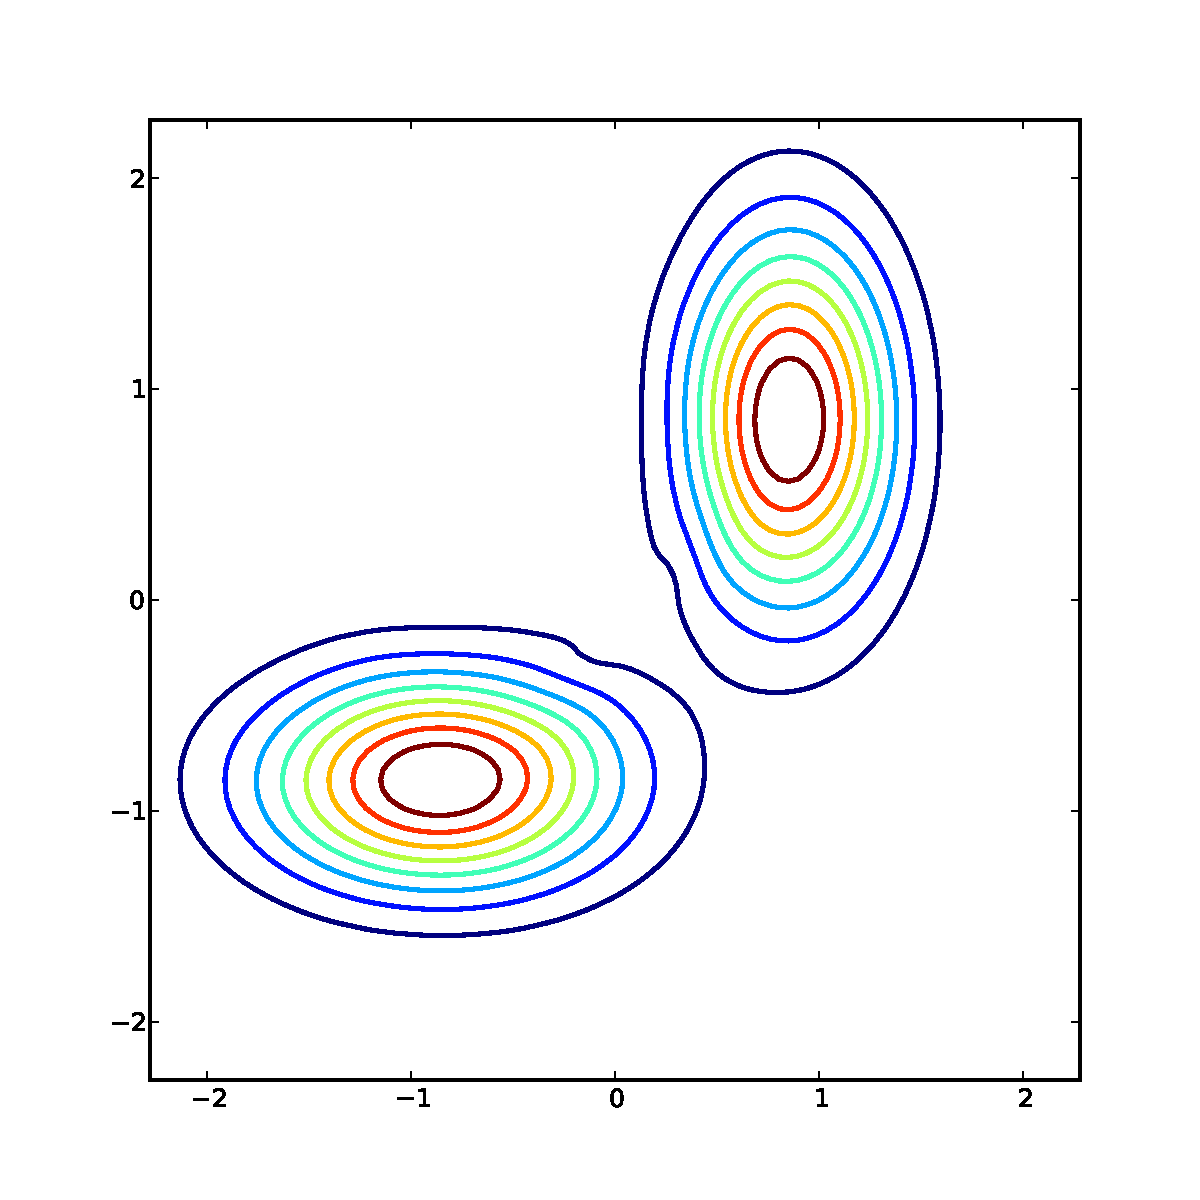
\includegraphics[width=4.2cm]{figs/polboltz/scrossed-b1-i0}
    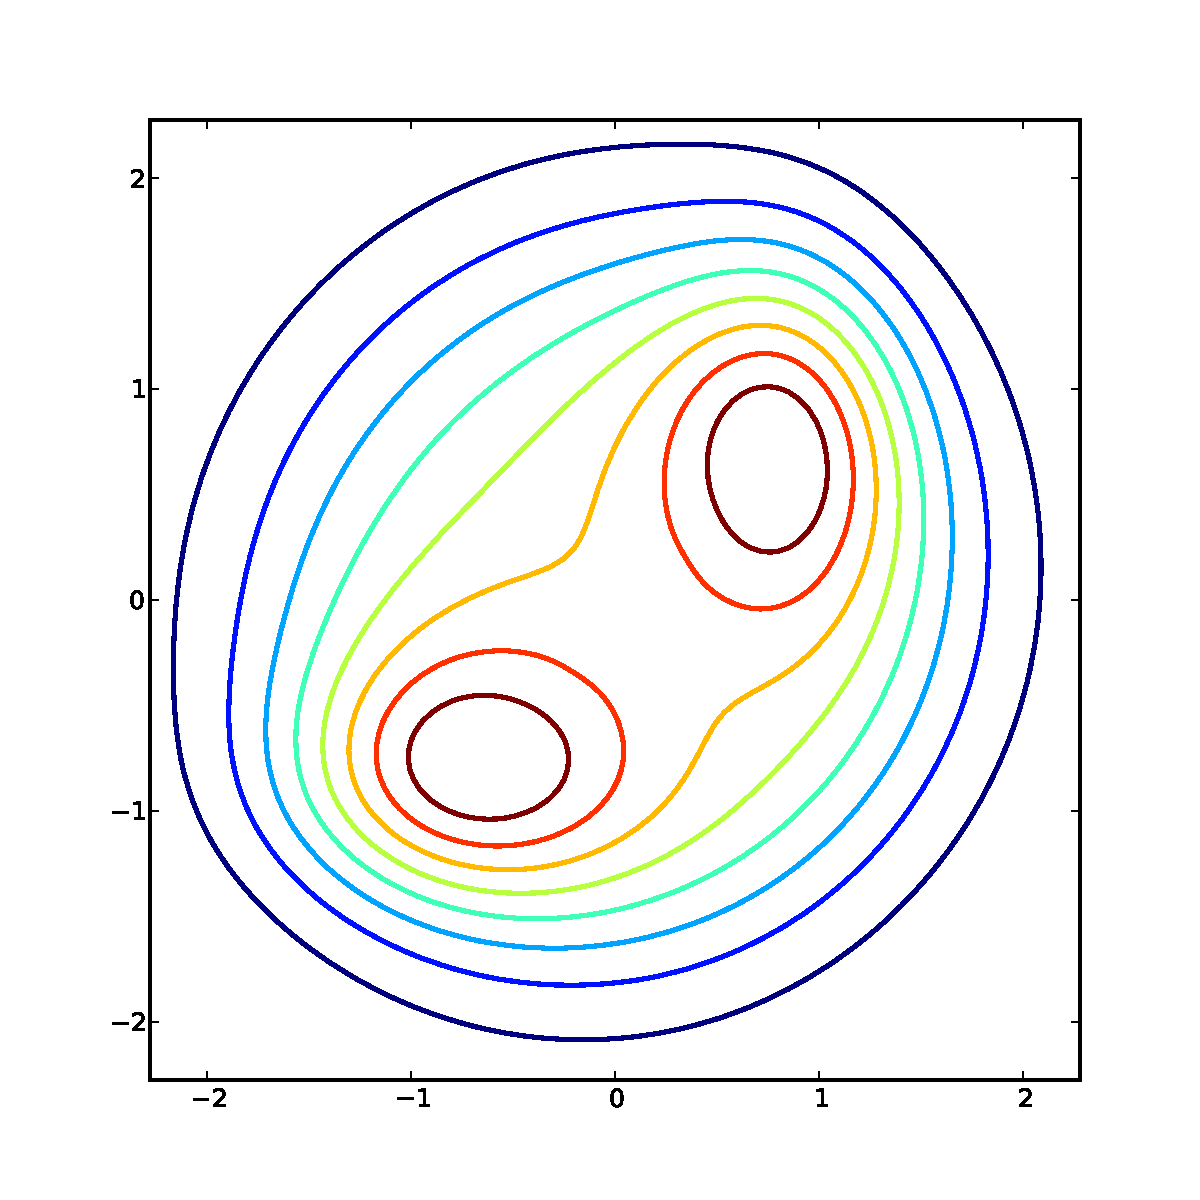
\includegraphics[width=4.2cm]{figs/polboltz/scrossed-b1-i2}
    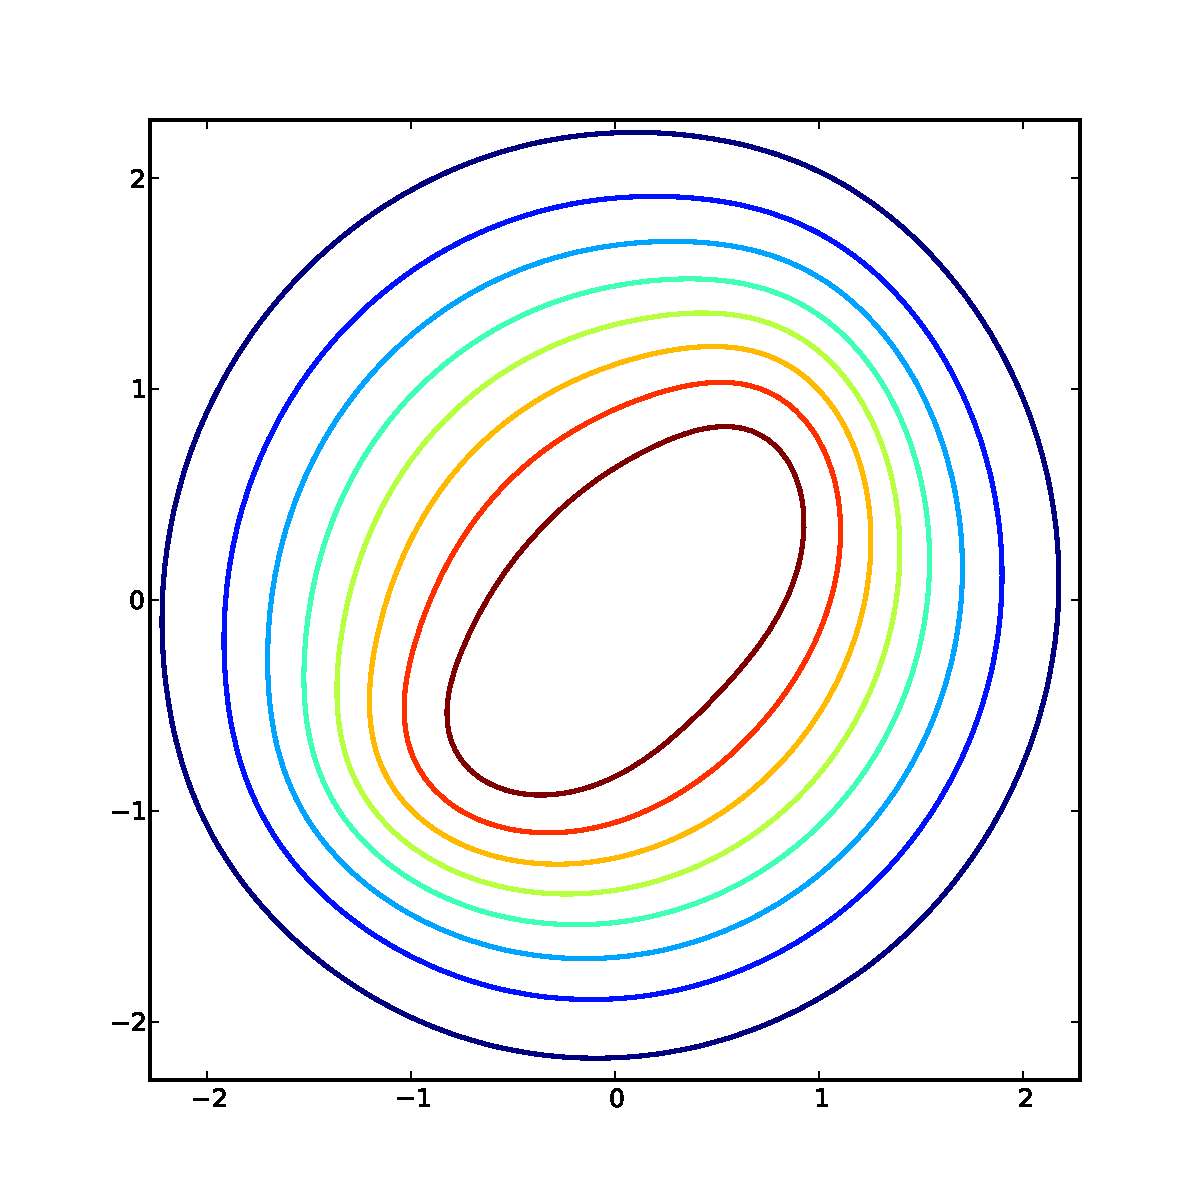
\includegraphics[width=4.2cm]{figs/polboltz/scrossed-b1-i3}
} \\
\subfloat[$\beta=2$]{
    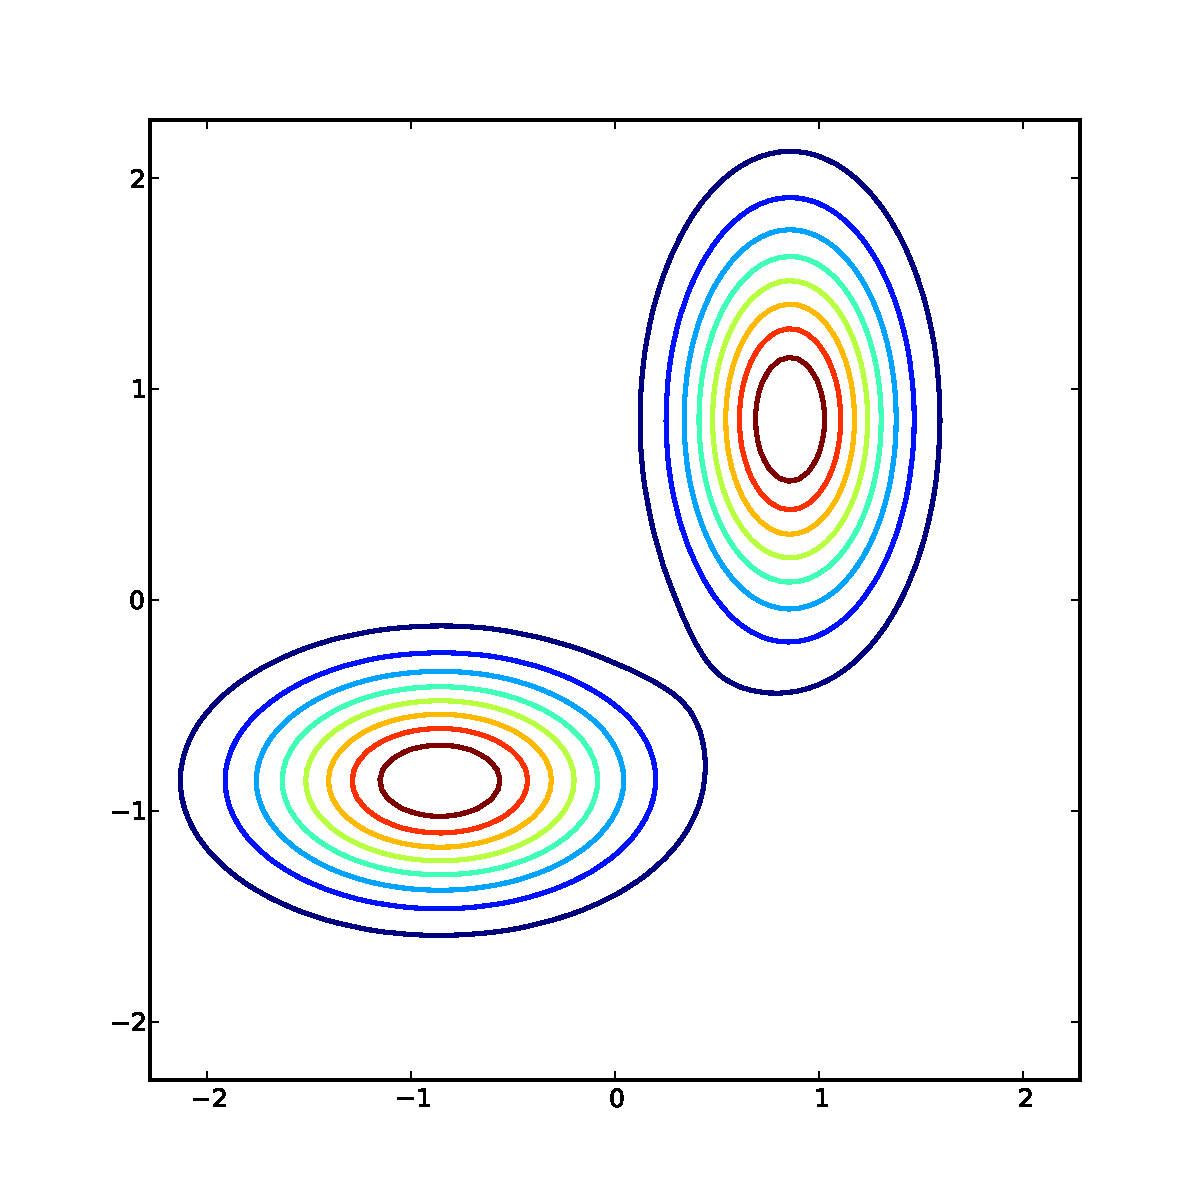
\includegraphics[width=4.2cm]{figs/polboltz/scrossed-b2-i0}
    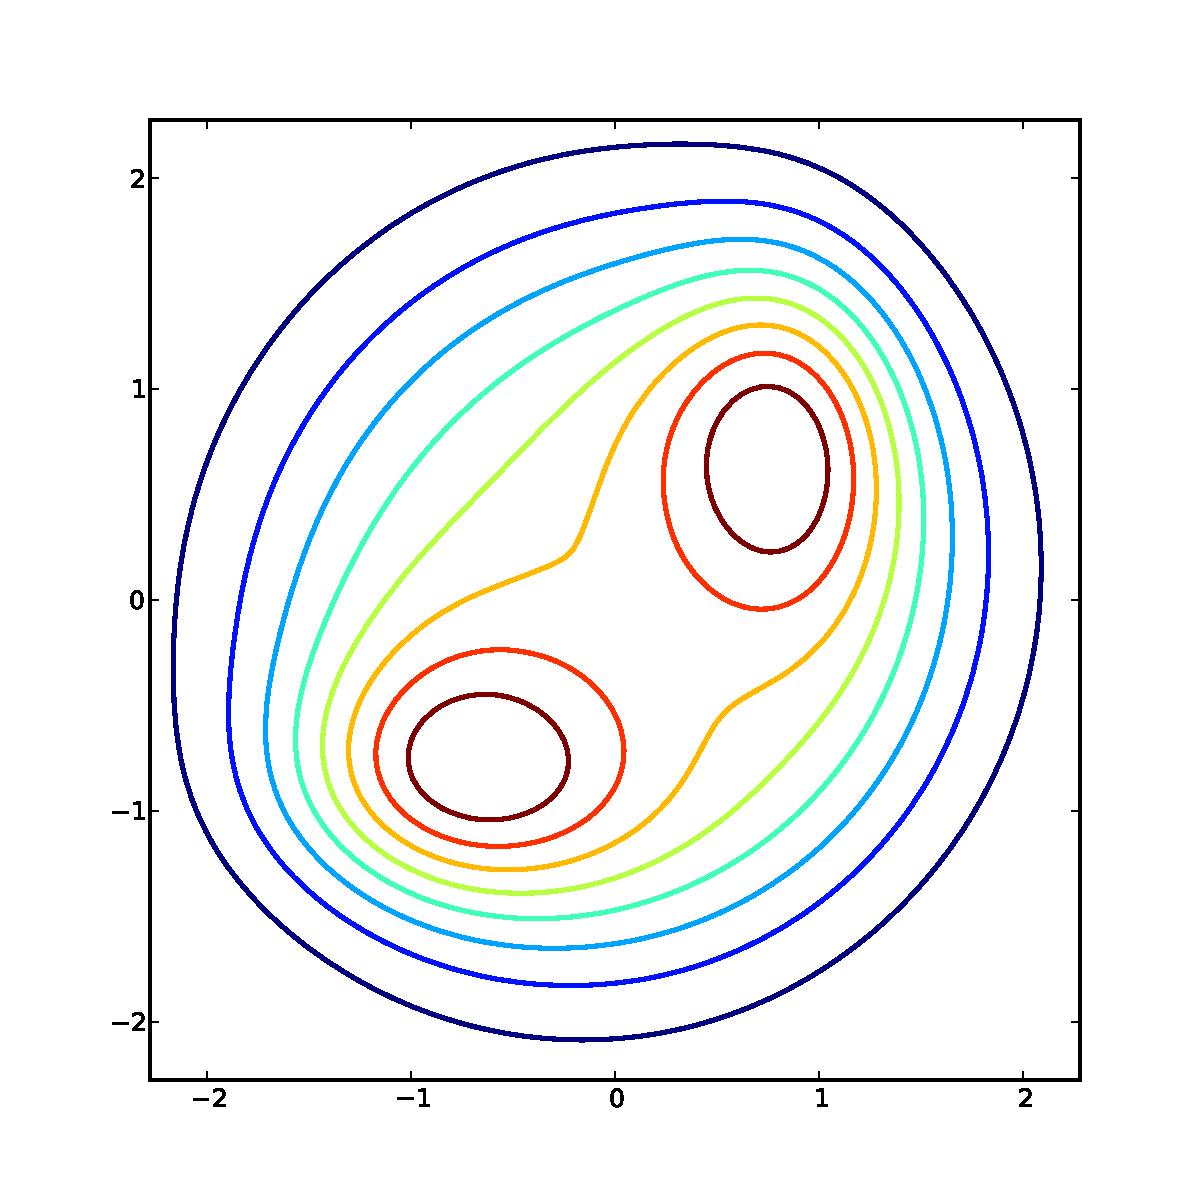
\includegraphics[width=4.2cm]{figs/polboltz/scrossed-b2-i2}
    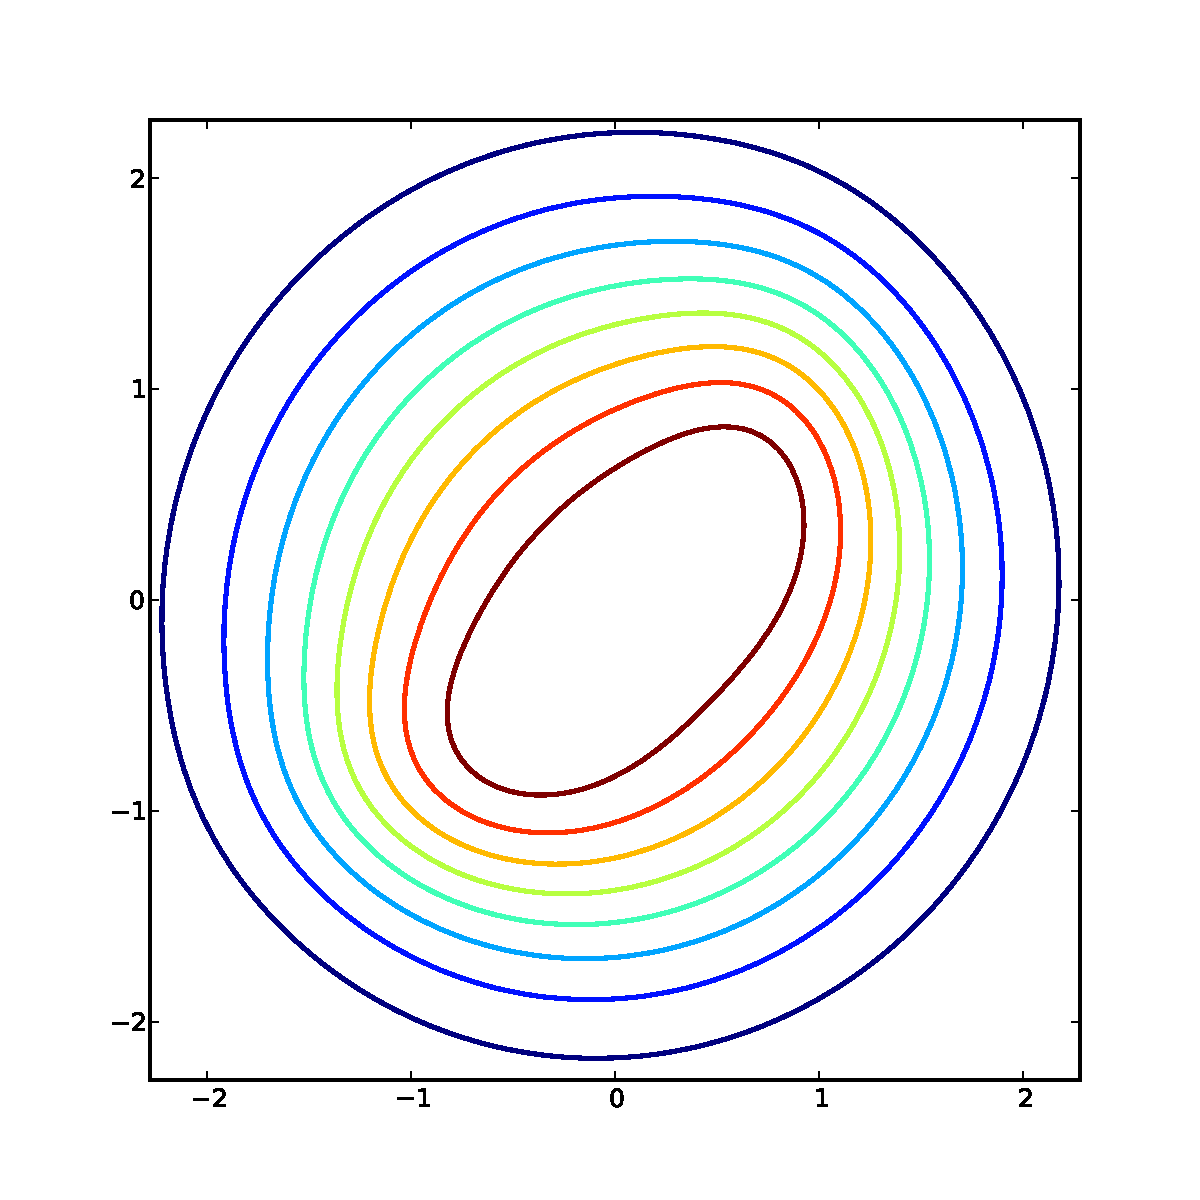
\includegraphics[width=4.2cm]{figs/polboltz/scrossed-b2-i3}
}
\caption{Solutions to the crossed streams experiment with $K=44$, $L=26$.  The times shown are, from left to
right, $t=0,\,0.5,\,0.75$. See Section~\vref{sec:numpol-cb} for details.}
\label{fig:numpol-cb}
\end{figure}

\begin{figure}
    \centering
    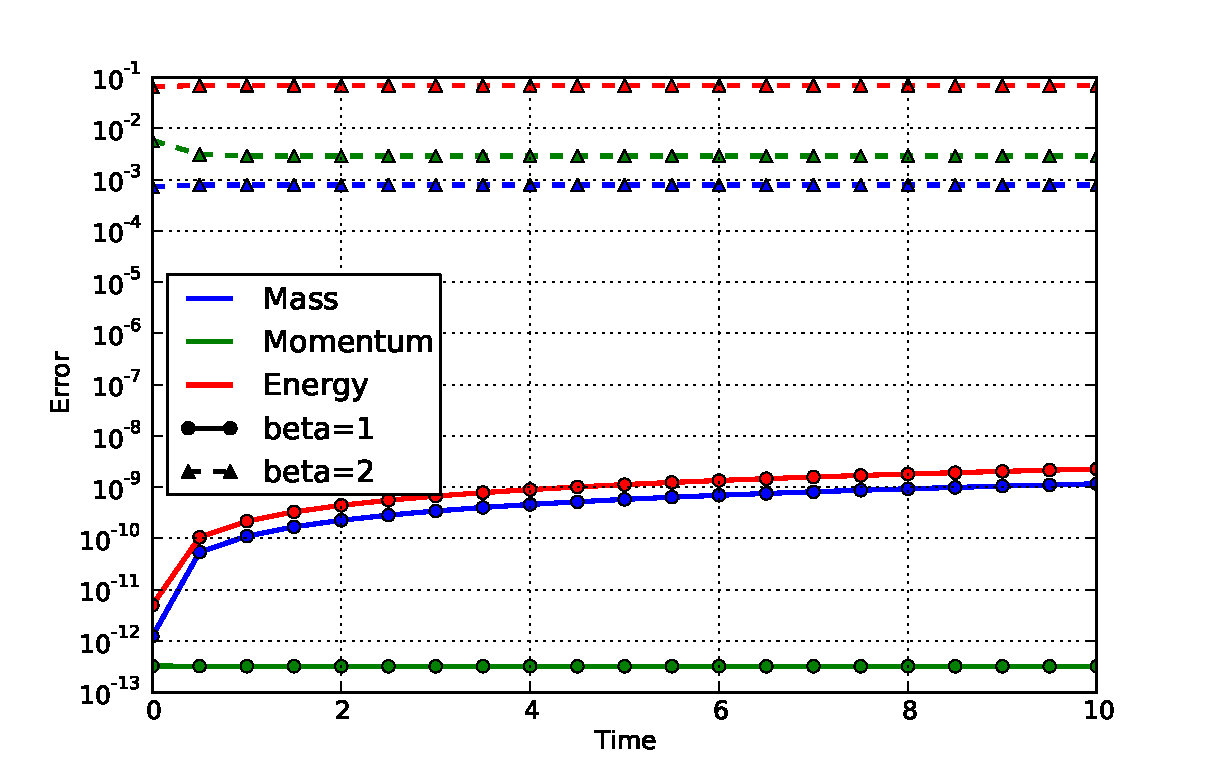
\includegraphics[width=12cm]{figs/polboltz/scrossed-obs}
    \caption{Error in observables at different times for the crossed streams experiment. The progressive
    worsening of mass density and energy for $\beta=1$ is attributed to quadrature error. See
    Section~\vref{sec:numpol-cb} for details.}
    \label{fig:numpol-cb-obs}
\end{figure}

\begin{figure}
\centering
\subfloat[$\beta=1$]{
    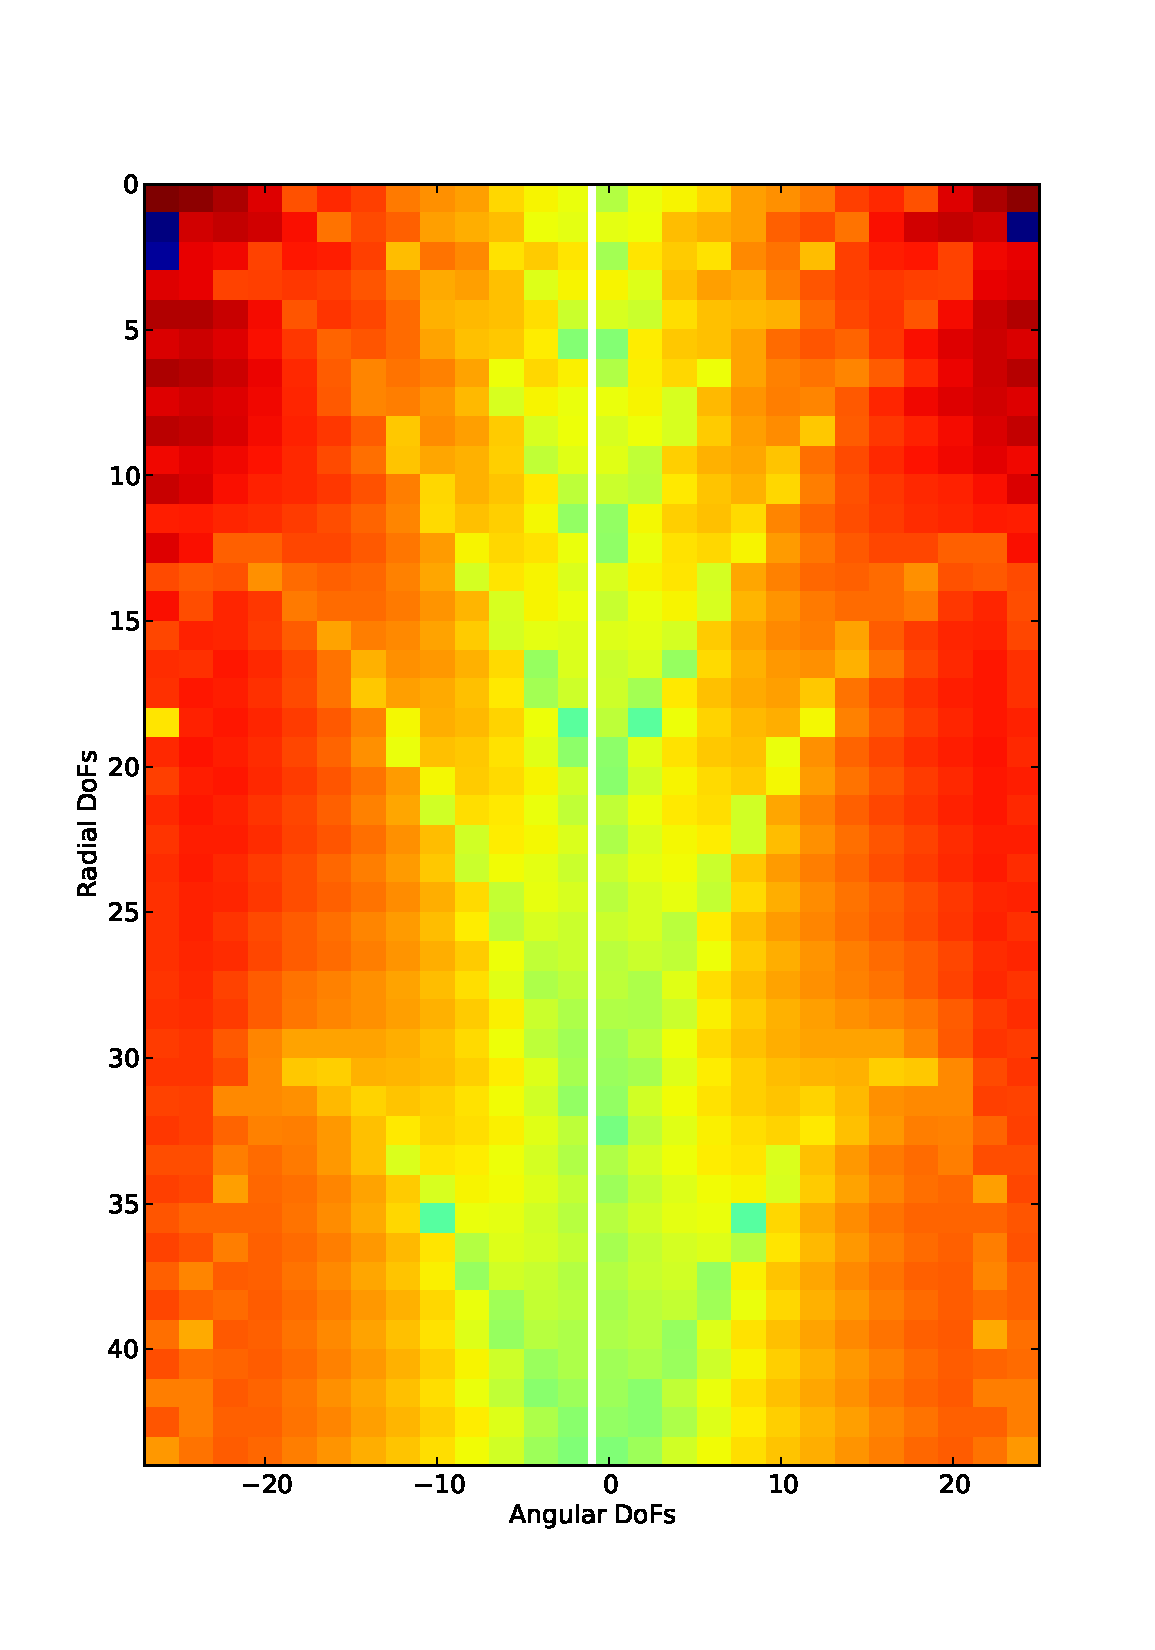
\includegraphics[width=4.2cm]{figs/polboltz/scrossed-spec-b1-i0}
    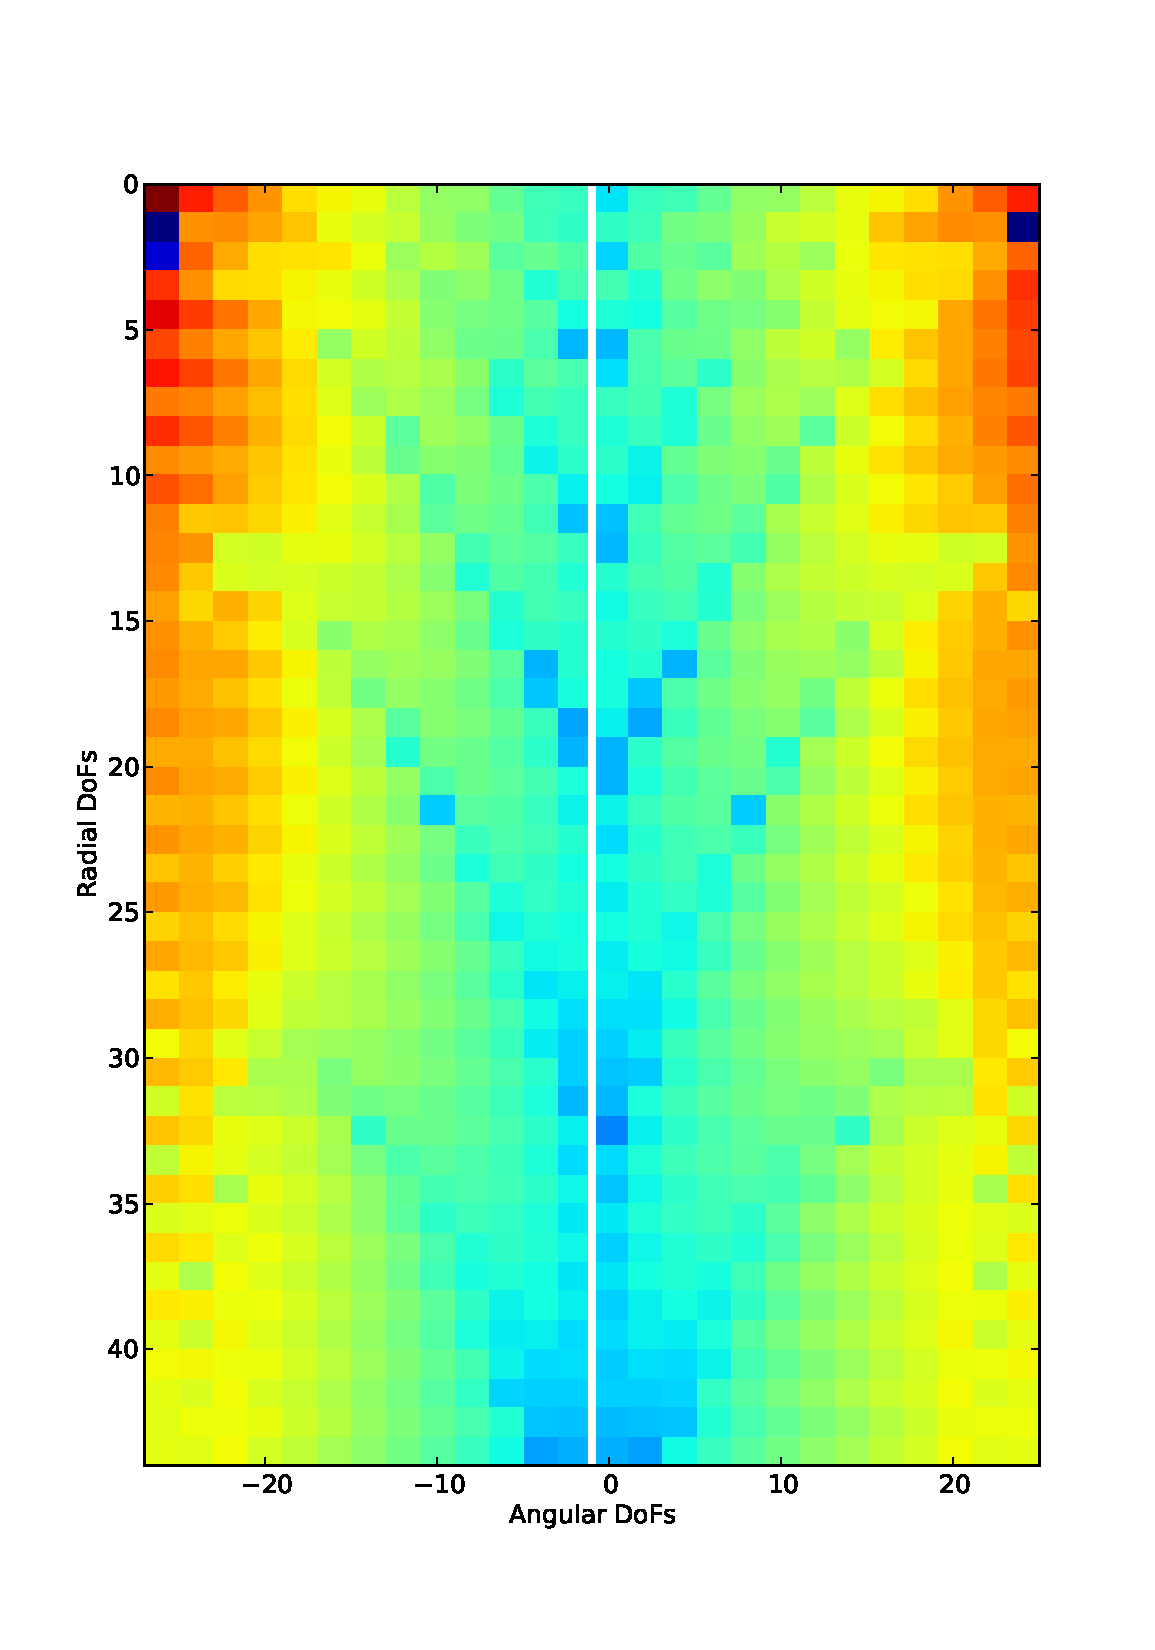
\includegraphics[width=4.2cm]{figs/polboltz/scrossed-spec-b1-i1}
    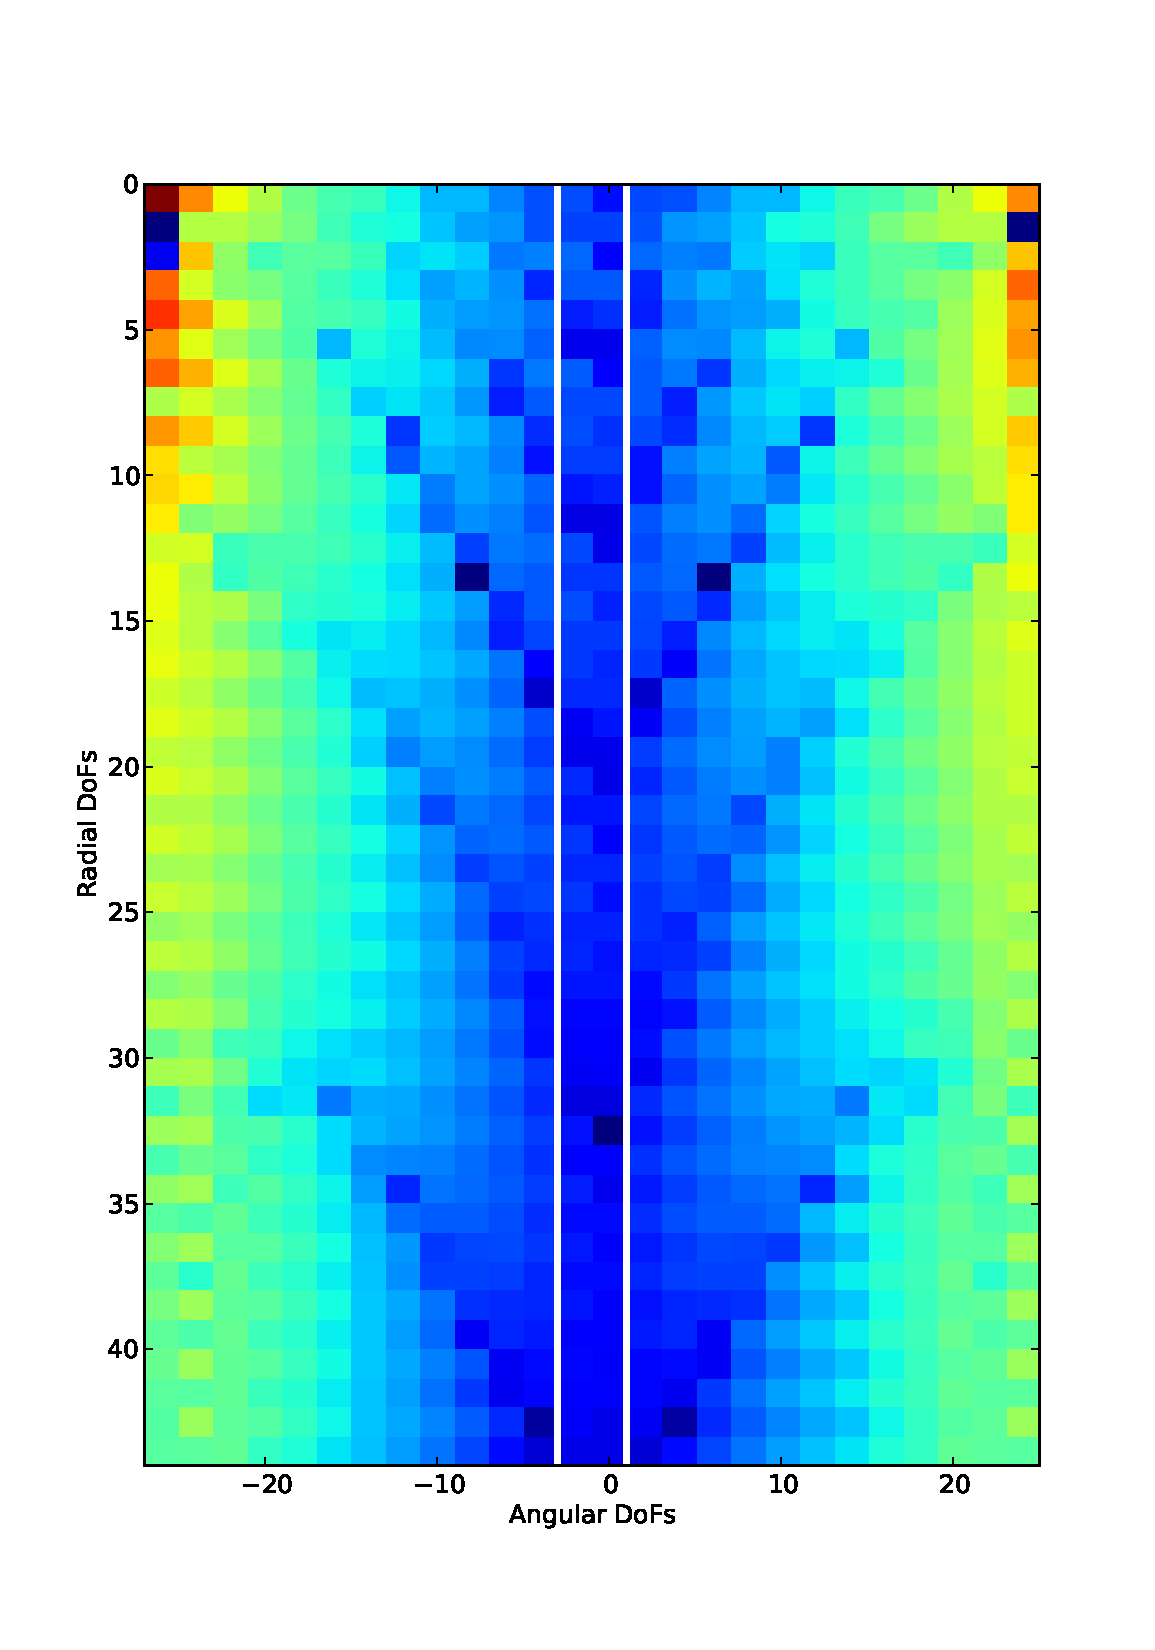
\includegraphics[width=4.2cm]{figs/polboltz/scrossed-spec-b1-i2}
} \\
\subfloat[$\beta=2$]{
    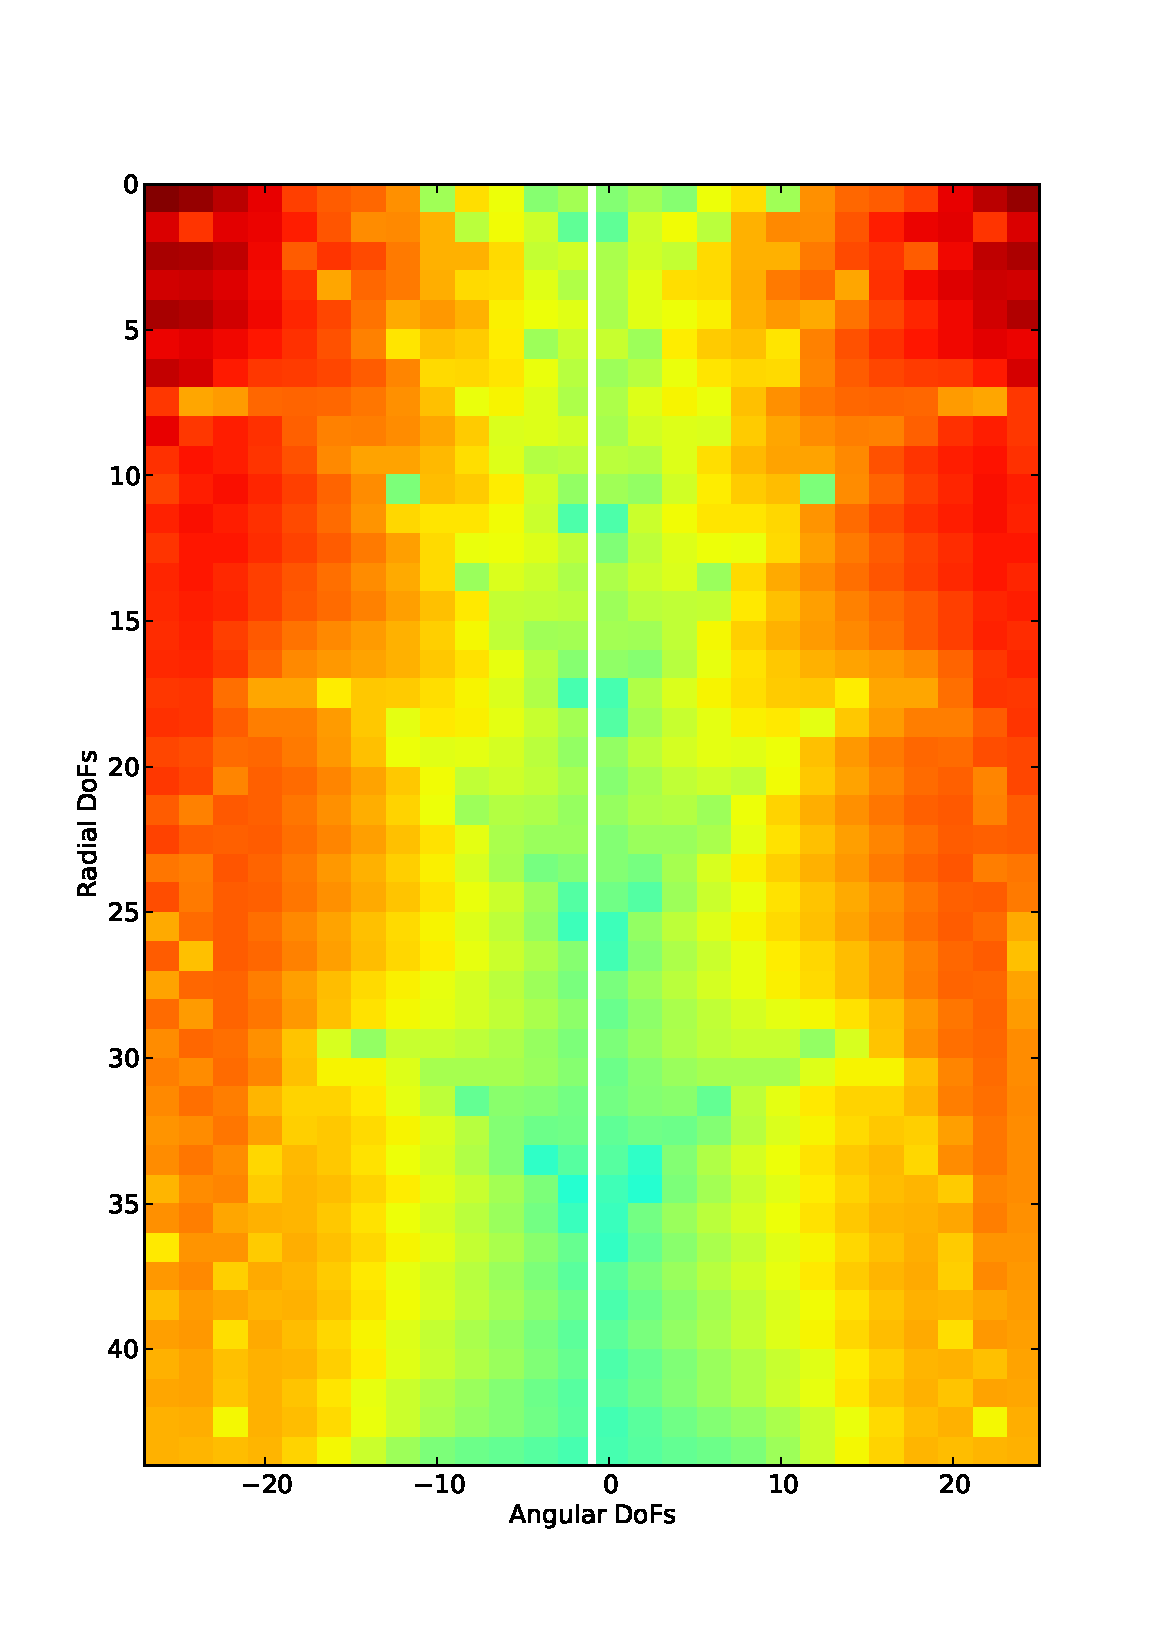
\includegraphics[width=4.2cm]{figs/polboltz/scrossed-spec-b2-i0}
    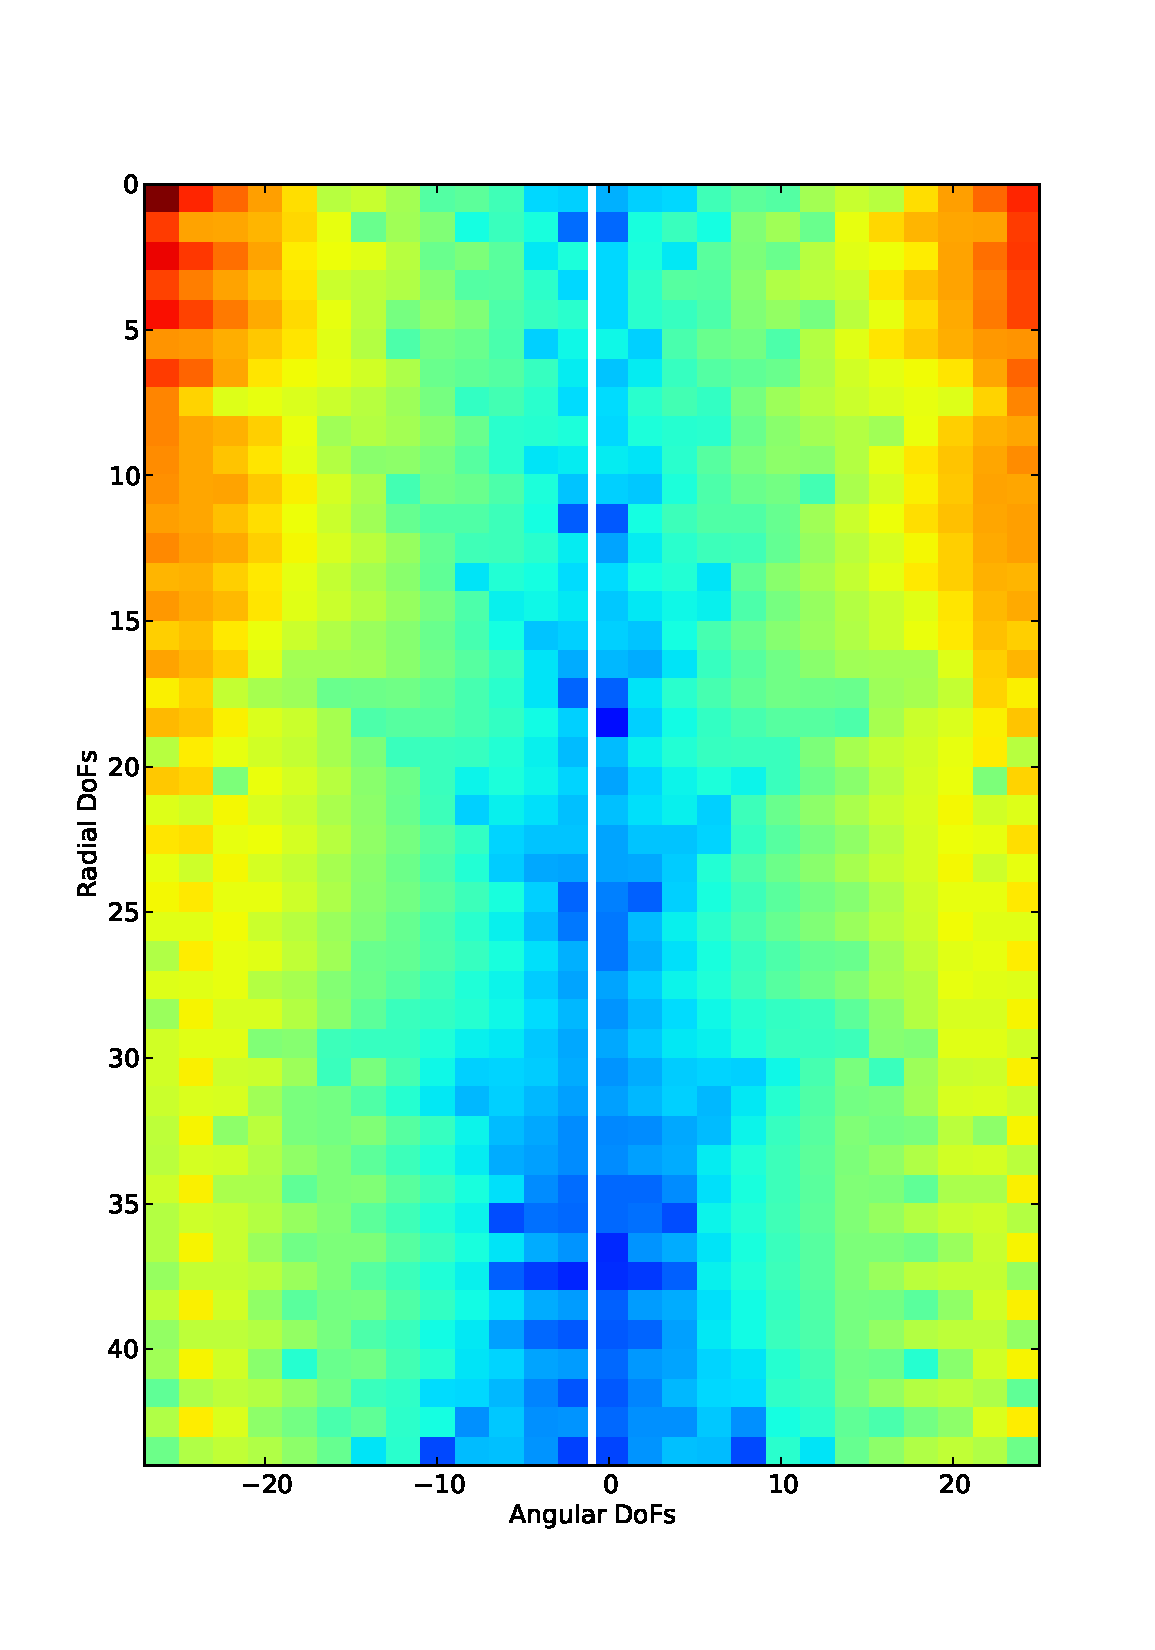
\includegraphics[width=4.2cm]{figs/polboltz/scrossed-spec-b2-i1}
    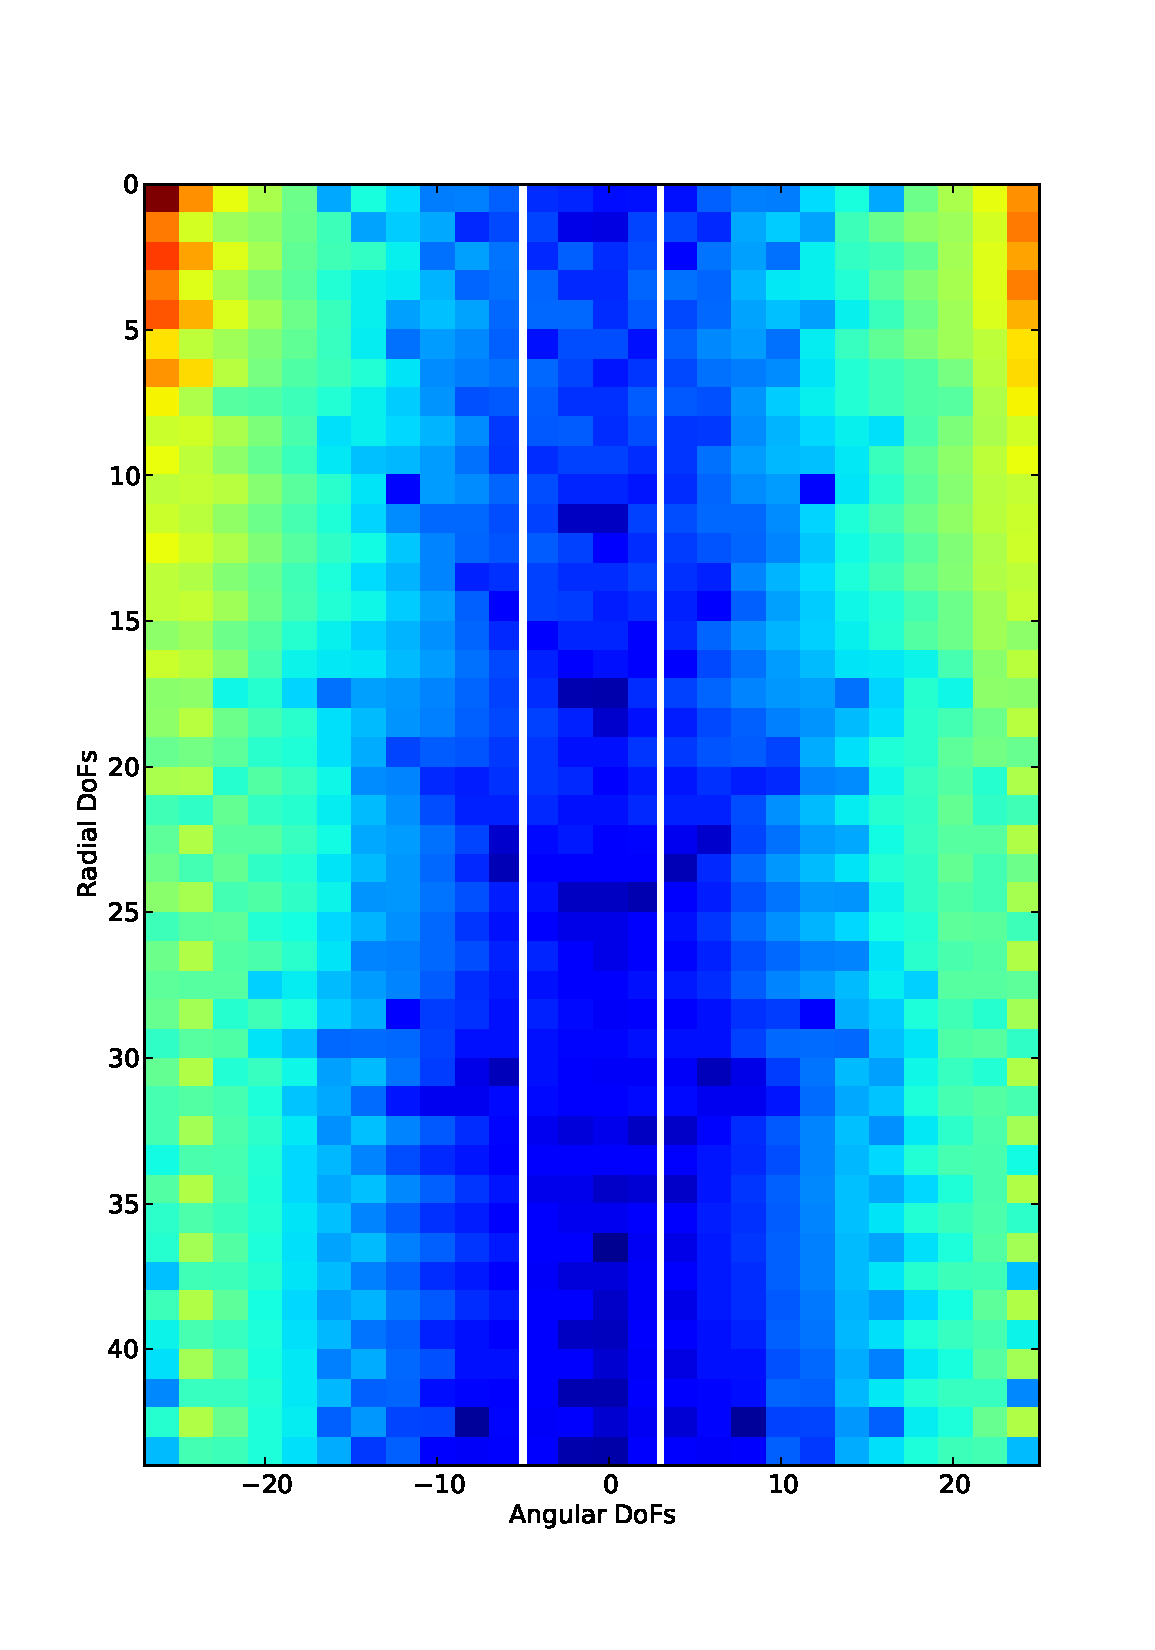
\includegraphics[width=4.2cm]{figs/polboltz/scrossed-spec-b2-i2}
}
\caption{Spectral magnitudes for the crossed streams experiment.  The times shown are, from left to right,
$t=0,\,2.1,\,4.2$.  The adaptive restriction of the function space is indicated with white lines,
using a threshold value of $10^{-10}$. See Section~\vref{sec:numpol-cb} for details.}
\label{fig:numpol-cb-spec}
\end{figure}

\begin{figure}
    \centering
    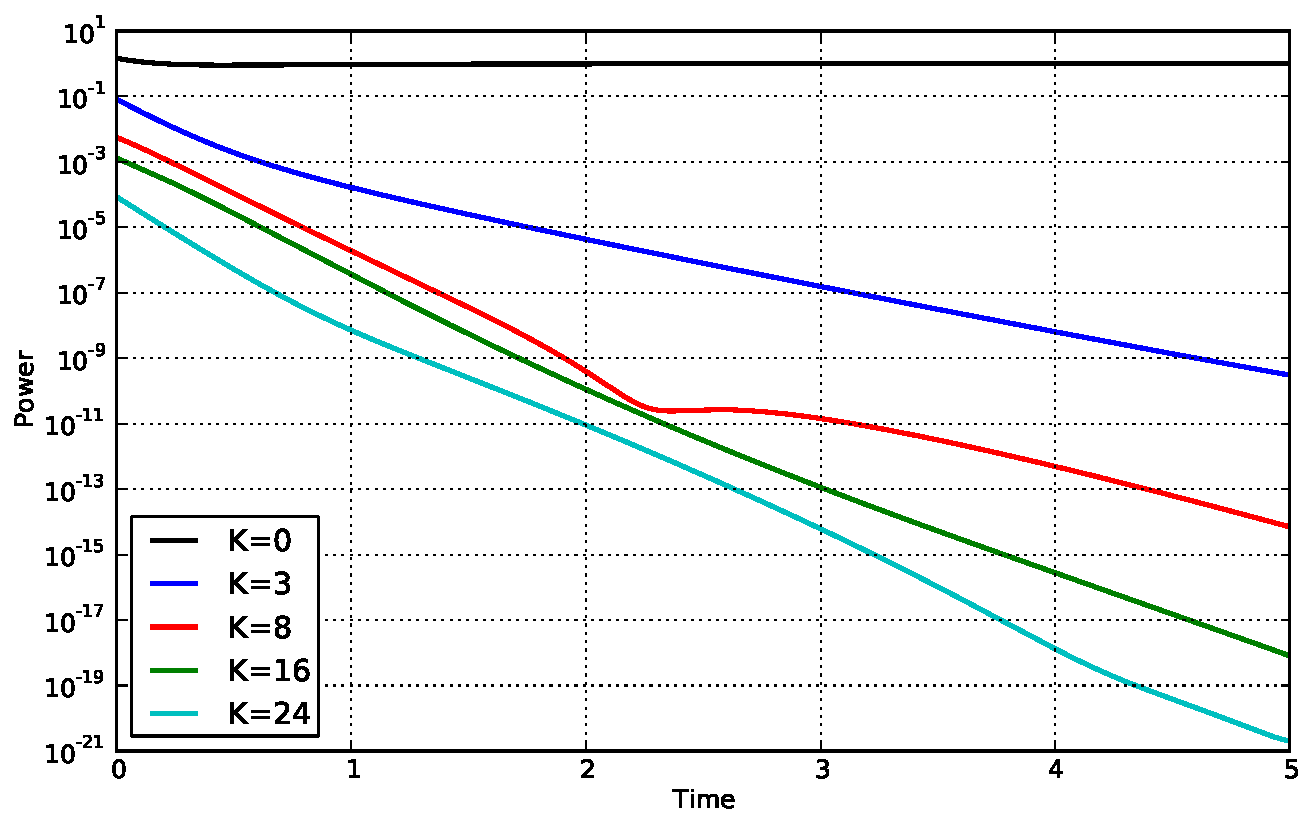
\includegraphics[width=10cm]{figs/polboltz/power}
    \caption{Power contribution for some values of $k$ for the crossed streams experiment. See
    Section~\vref{sec:numpol-cb} for details.}
    \label{fig:numpol-cb-power}
\end{figure}

\begin{figure}
    \centering
    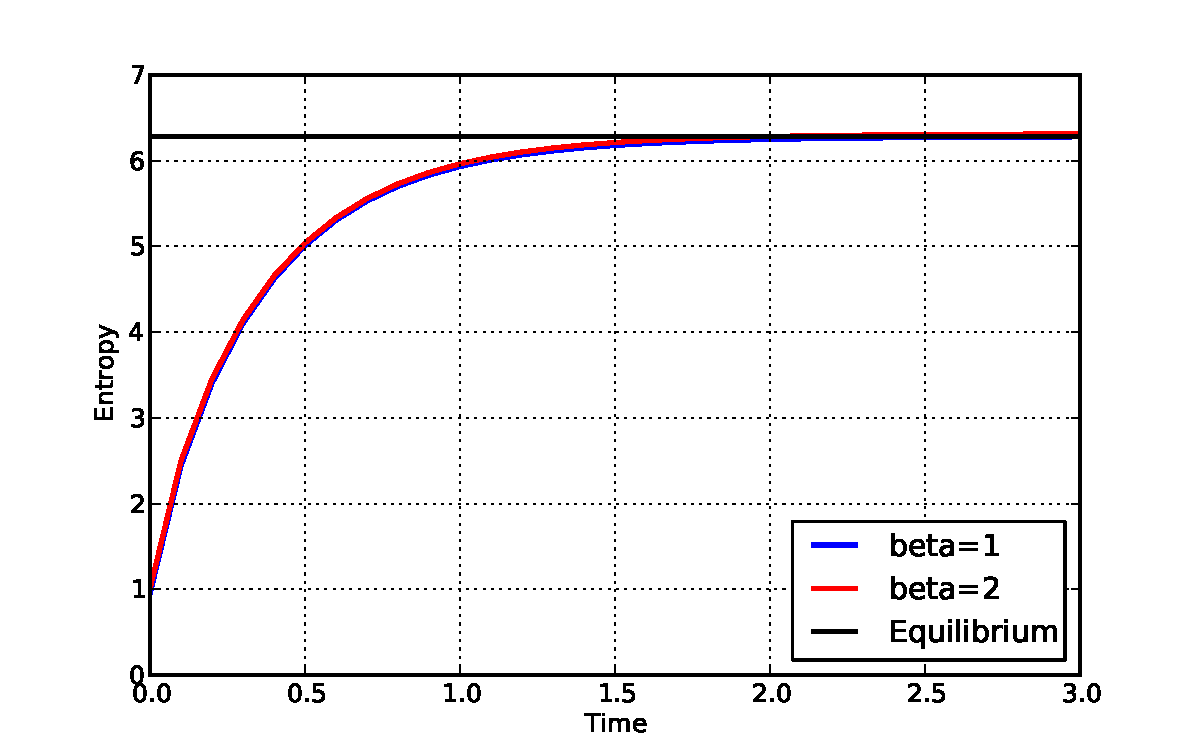
\includegraphics[width=12cm]{figs/polboltz/scrossed-ent}
    \caption{Entropy as a function of time for the crossed streams experiment. See
    Section~\vref{sec:numpol-cb} for details.}
    \label{fig:numpol-cb-ent}
\end{figure}

\clearpage

\subsection{Adaptivity} \label{sec:numpol-adapt}

In Figure~\vref{fig:numpol-adapt} we show the time-dependence of the computational effort per timestep (a
pseudo-quantity of $L^2$), under the strategy detailed in Section~\vref{sec:pol-adapt}. The results shown are
for three different experiments, one of which (blue) is the crossed streams of the previous section. In this
particular case we used a threshold value of $10^{-10}$, which can be considered very strict.

We observe a strong downward tendency in all cases. One achieves better adaptivity for $\beta=2$ than
$\beta=1$, but this difference does not appear to be significant compared to the dependence on the actual
initial data.

\begin{figure}
    \centering
    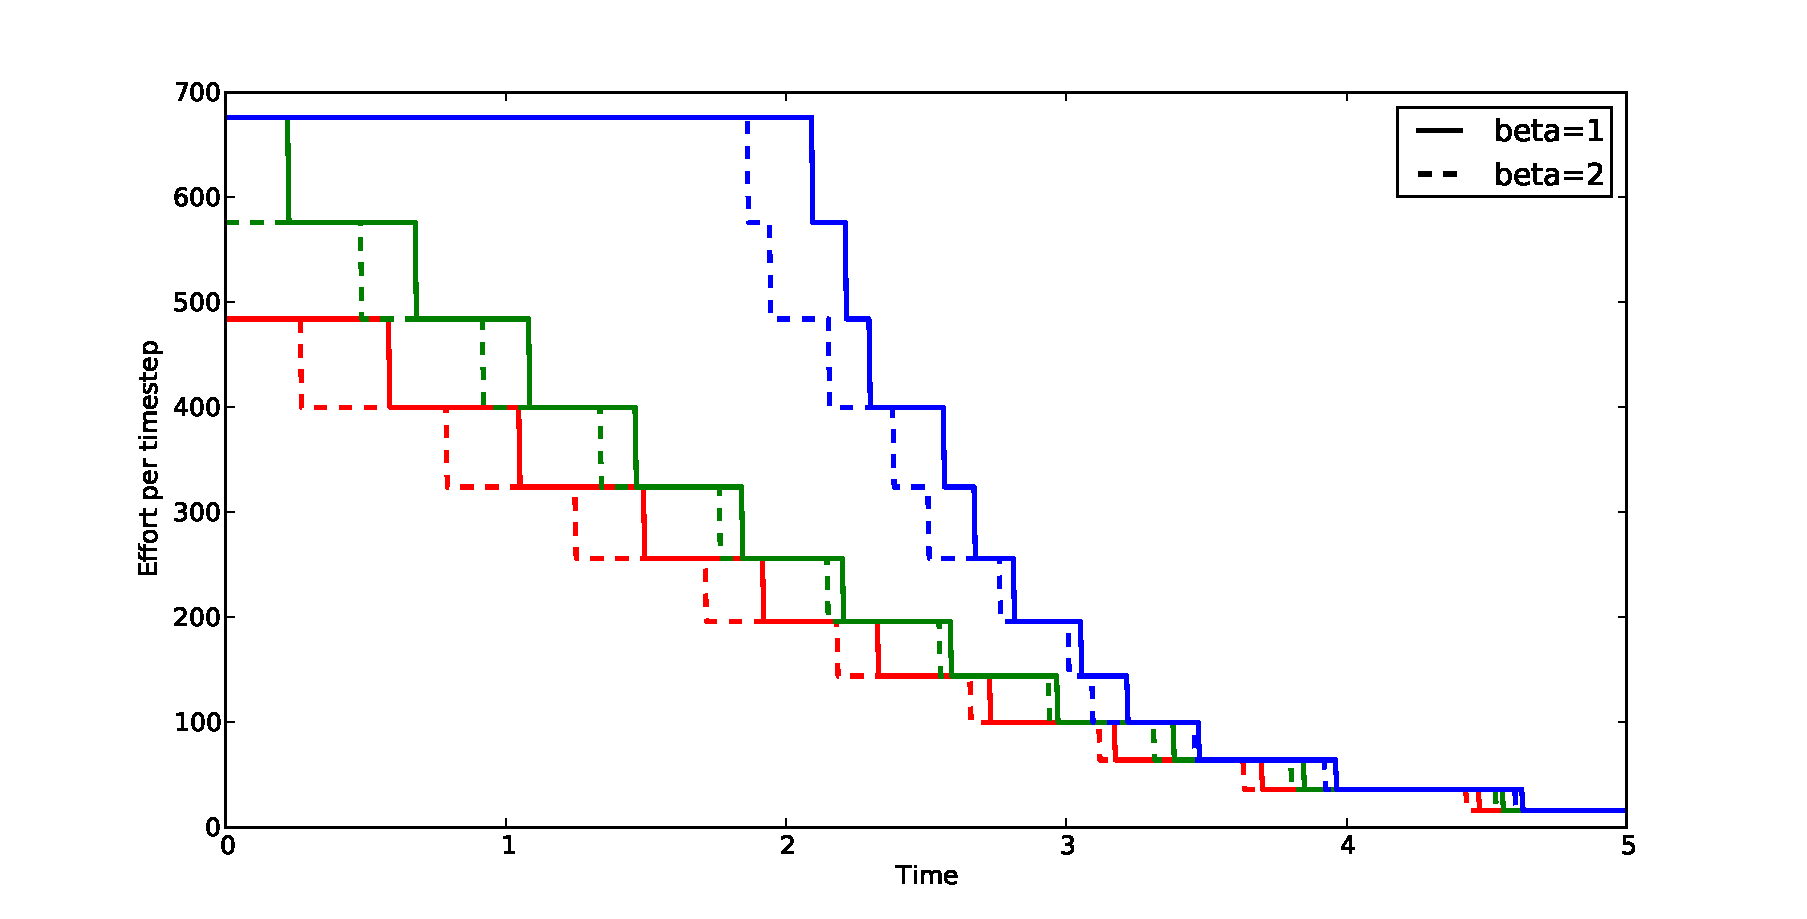
\includegraphics[width=14cm]{figs/polboltz/adapt}
    \caption{Time-dependence of computational effort per timestep ($\propto L^2$) for three different
    experiments (red is the crossed streams solution of Section~\vref{sec:numpol-cb}, blue is the initial
    condition $\frac{5}{4}\exp(-\frac{5}{16}(4v_x^2+v_y^2))$, and green is the initial condition
    $\alpha\left[\exp(-\alpha|\Bv-\eta|^2) + \frac{1}{2}\exp(-\frac{\alpha}{2}|\Bv+\eta|^2)\right]$ where
    $S=1.8$, $\alpha=\frac{1}{4}(3+2S^2)$ and $\eta=S\alpha^{-\nicefrac{1}{2}}$. (The latter two are given in
    their $\beta=2$-conforming cases.) See Section~\vref{sec:numpol-adapt} for details.}
    \label{fig:numpol-adapt}
\end{figure}

\subsection{Collision tensor compressibility} \label{sec:coltens-comp}

Figure~\vref{fig:coltens-comp} shows the magnitude of the nonzero collision tensor entries for $K=44$ and
$L=26$ (giving about $20$ million nonzero entries) for both $\beta=1$ and $\beta=2$. One might hope that a
sufficiently rapid decay in these entries can yield some compressibility of the tensor, but this appears not
to be the case, particularly not for $\beta=2$.

\begin{figure}
    \centering
    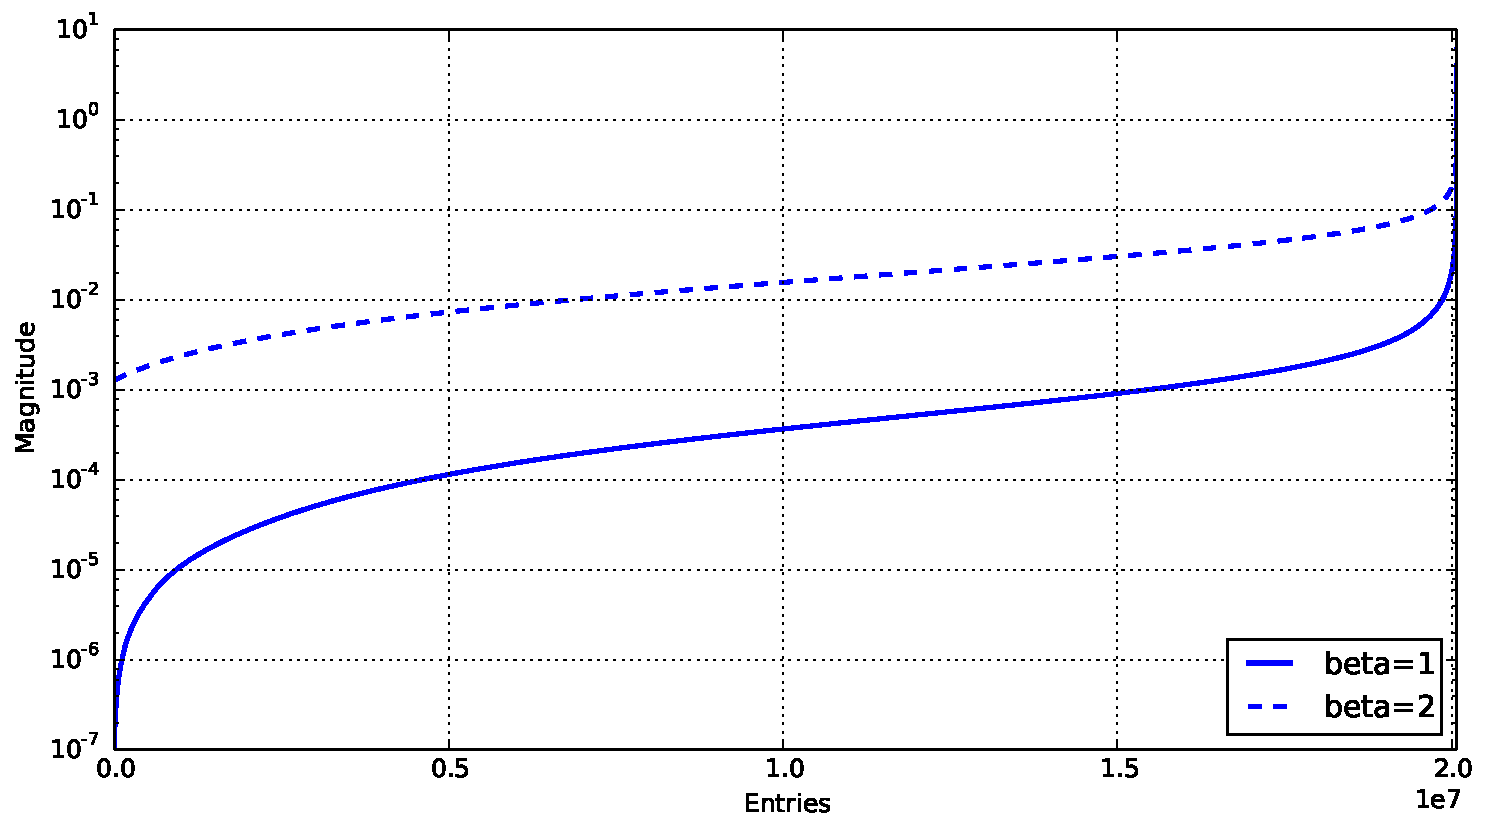
\includegraphics[width=12cm]{figs/polboltz/spectrum}
    \caption{Magnitudes of the roughly $20$ million nonzero collision tensor entries for $K=44$ and $L=26$.
    See Section~\vref{sec:coltens-comp} for details.}
    \label{fig:coltens-comp}
\end{figure}

\subsection{Non-conforming solutions} \label{sec:nonconf}

In light of the discussion in Section~\vref{sec:pol-inhom}, we study here the performance of the Polar method
for a non-conforming solution which has off-center momentum. The equilibrium solution is thus neither in the
solution space, nor is it isotropic. Specifically, we have used the initial condition
\[
    f_0(\Bv) = \exp\left[-5|\Bv|^2\right] + \exp\left[-5(v_x-1)^2-12v_y^2\right],
\]
which represents a stream of gas colliding with gas at equilibrium.

Figure~\vref{fig:numpol-nc} shows contour plots of the solutions to this experiment at various times for both
$\beta=1$ and $\beta=2$.

Figure~\vref{fig:numpol-nc-spec} shows the evolution of the spectral coefficients, and should be compared to
Figure~\vref{fig:numpol-cb-spec}. The general pattern of coefficient decay appears to be maintained, although
it is considerably slower, and will not go as far.

Finally, Figure~\vref{fig:numpol-nc-power} shows the time-dependent power contribution for some values of $k$,
for $\beta=2$, and should be compared to Figure~\vref{fig:numpol-cb-power}. The power content of the higher
levels can be seen to deteriorate for longer times in the $\beta=2$ case, which might be related to the poor
stability of the method and the lack of symmetry of the solution. The $\beta=1$ solutions suffer no such
effects.

\begin{figure}
\centering
\subfloat[$\beta=1$]{
    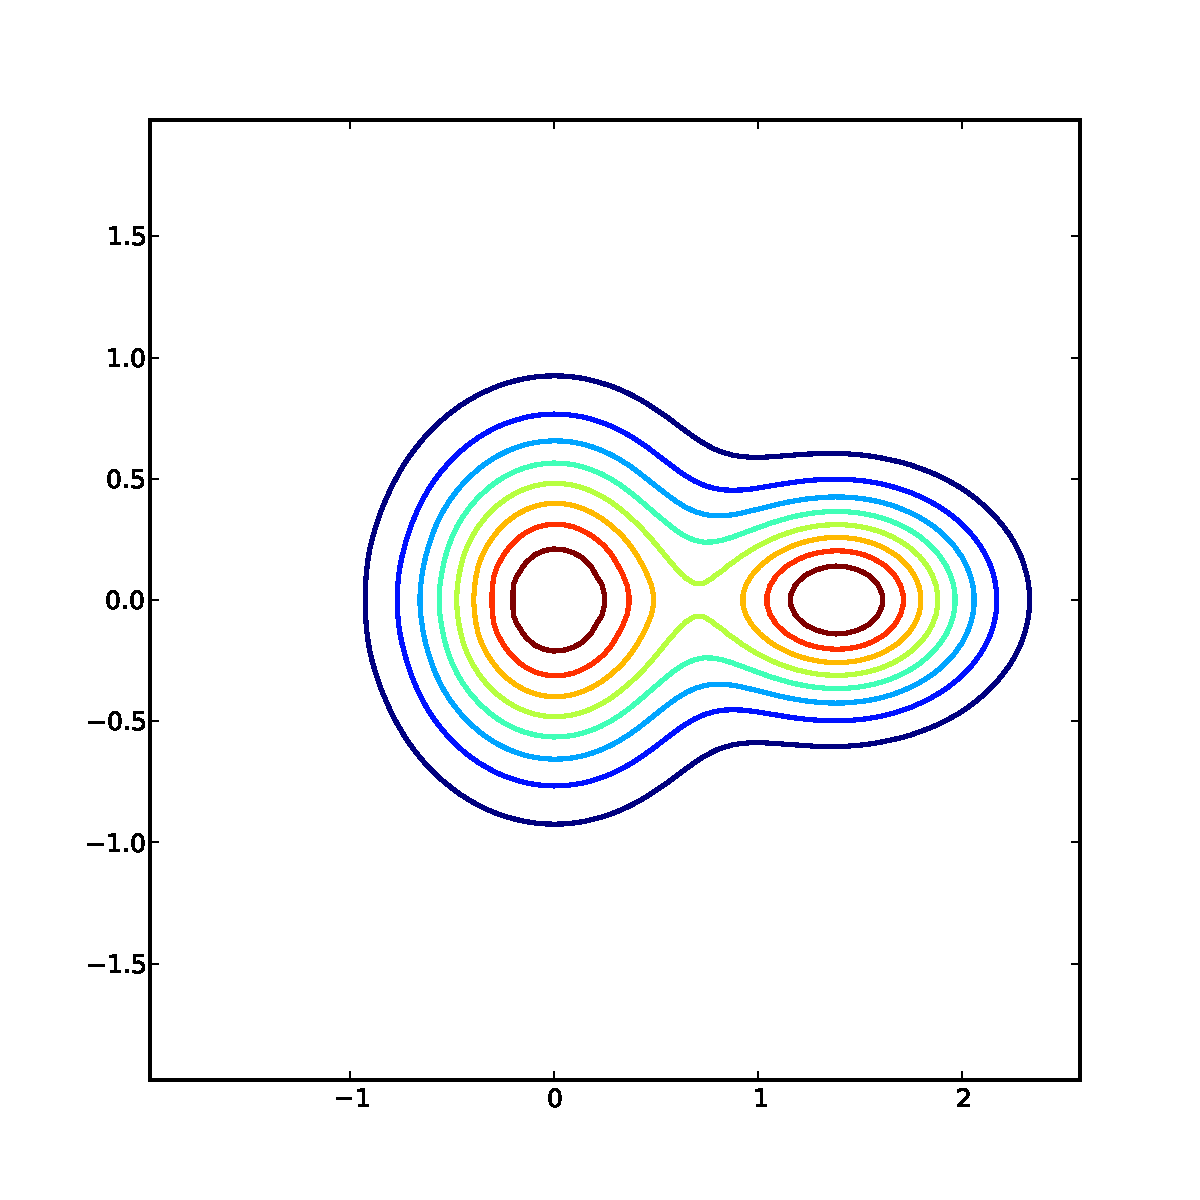
\includegraphics[width=4.2cm]{figs/polboltz/comp2-b1-i0}
    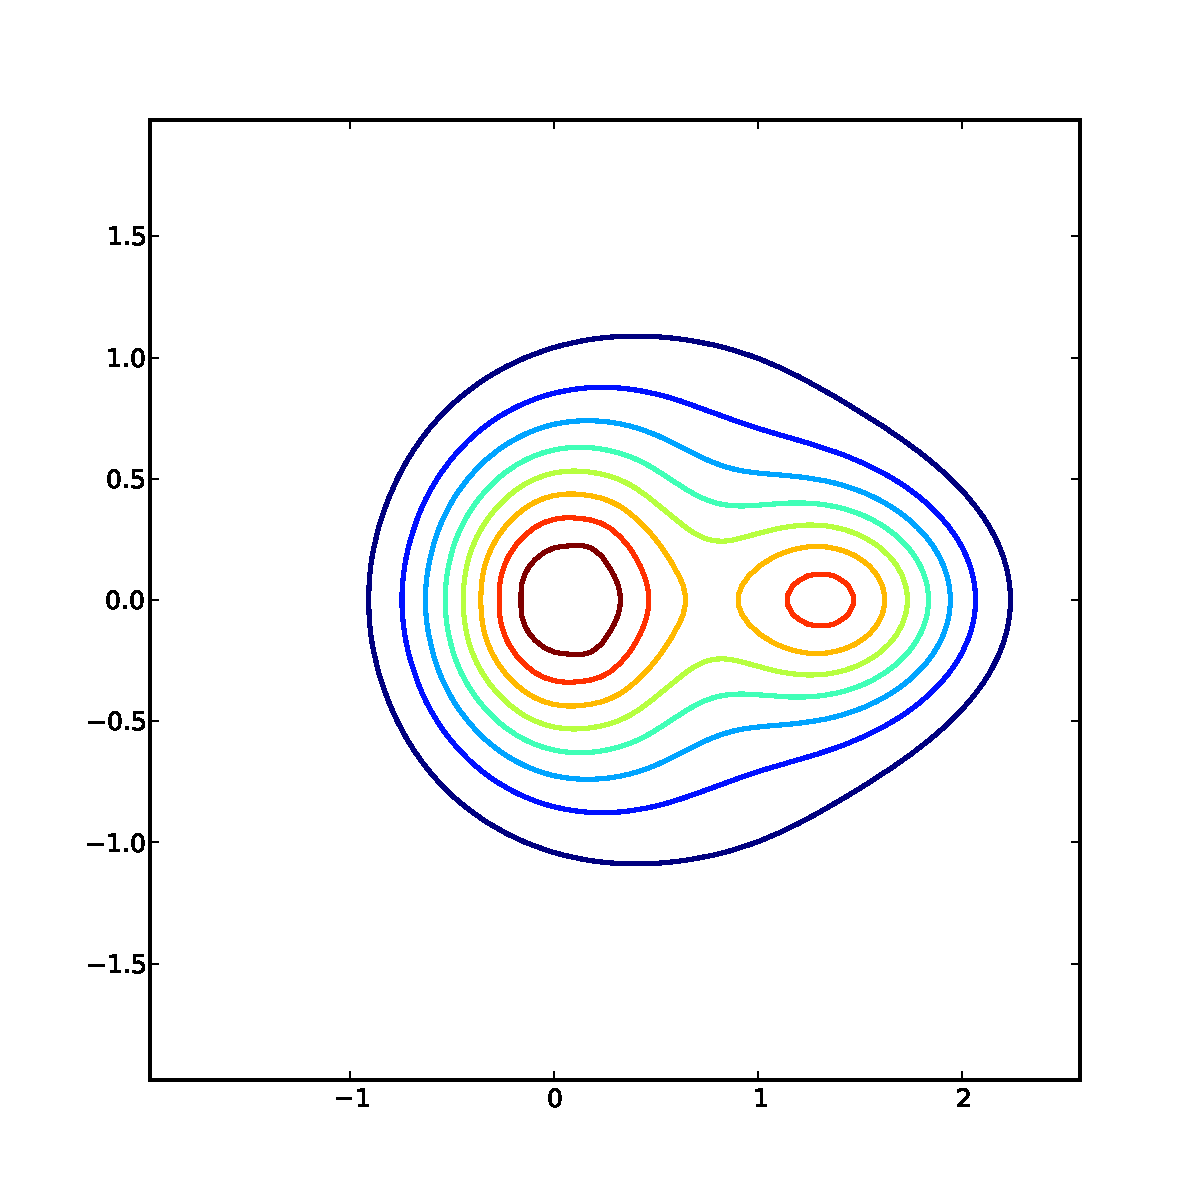
\includegraphics[width=4.2cm]{figs/polboltz/comp2-b1-i1}
    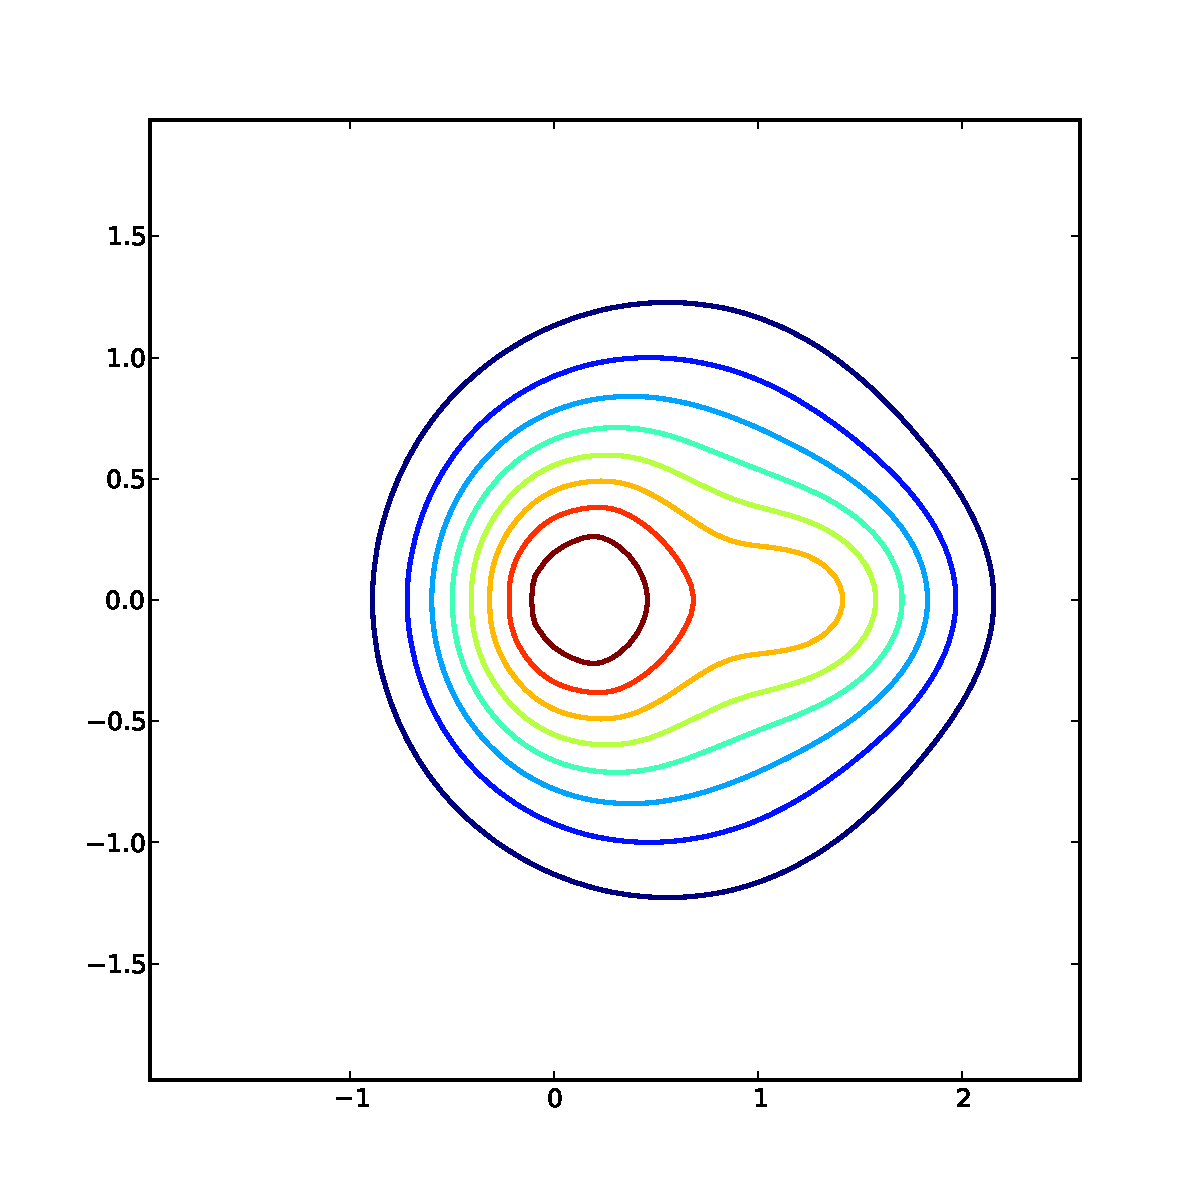
\includegraphics[width=4.2cm]{figs/polboltz/comp2-b1-i2}
} \\
\subfloat[$\beta=2$]{
    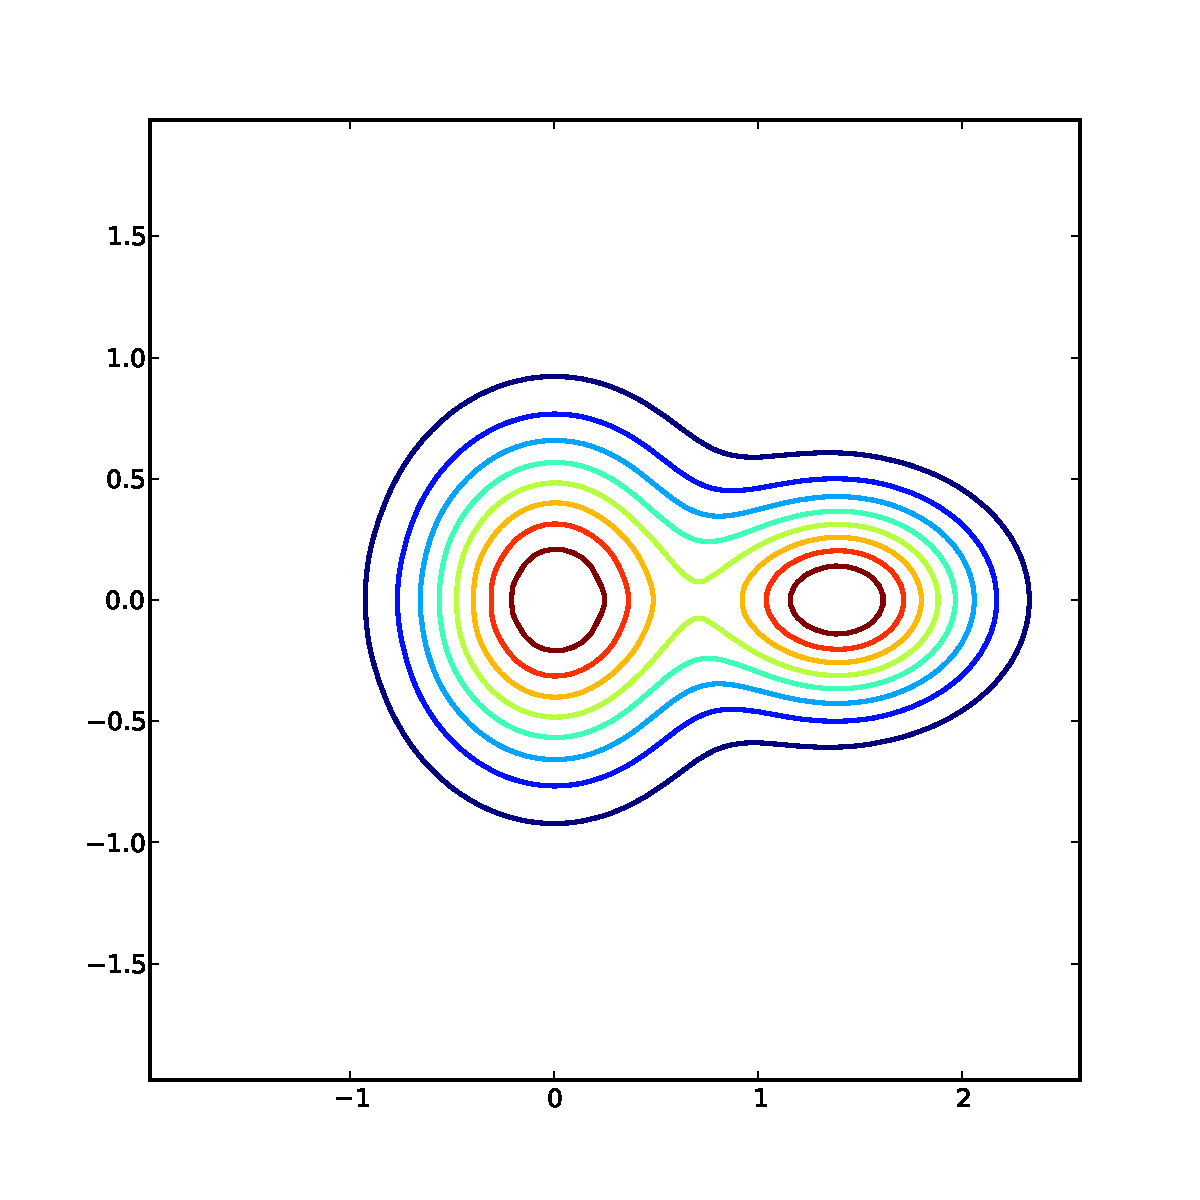
\includegraphics[width=4.2cm]{figs/polboltz/comp2-b2-i0}
    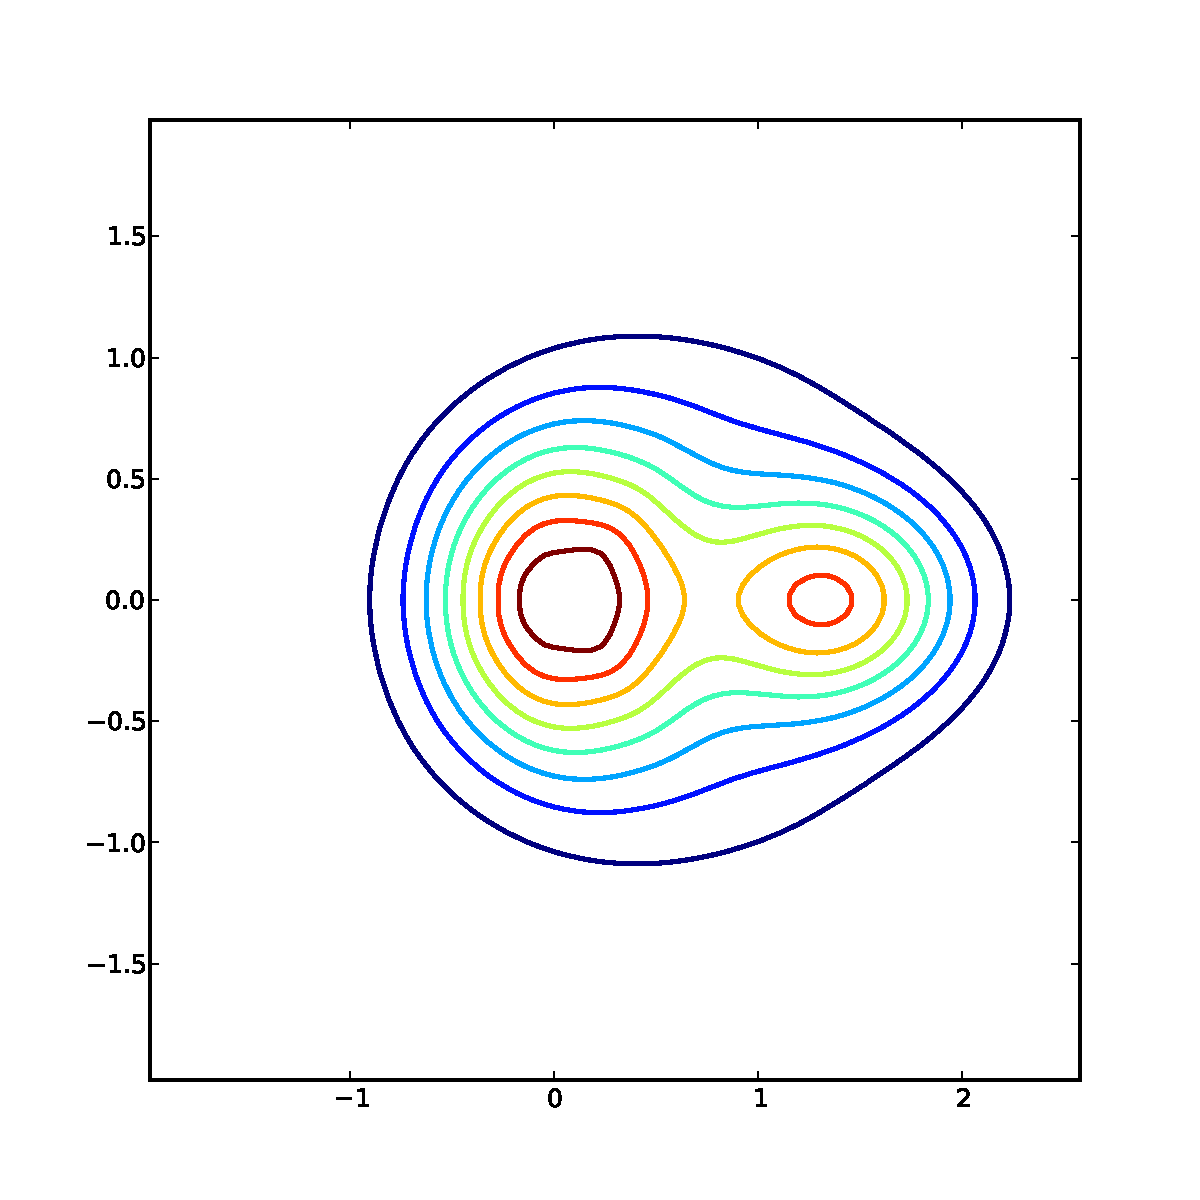
\includegraphics[width=4.2cm]{figs/polboltz/comp2-b2-i1}
    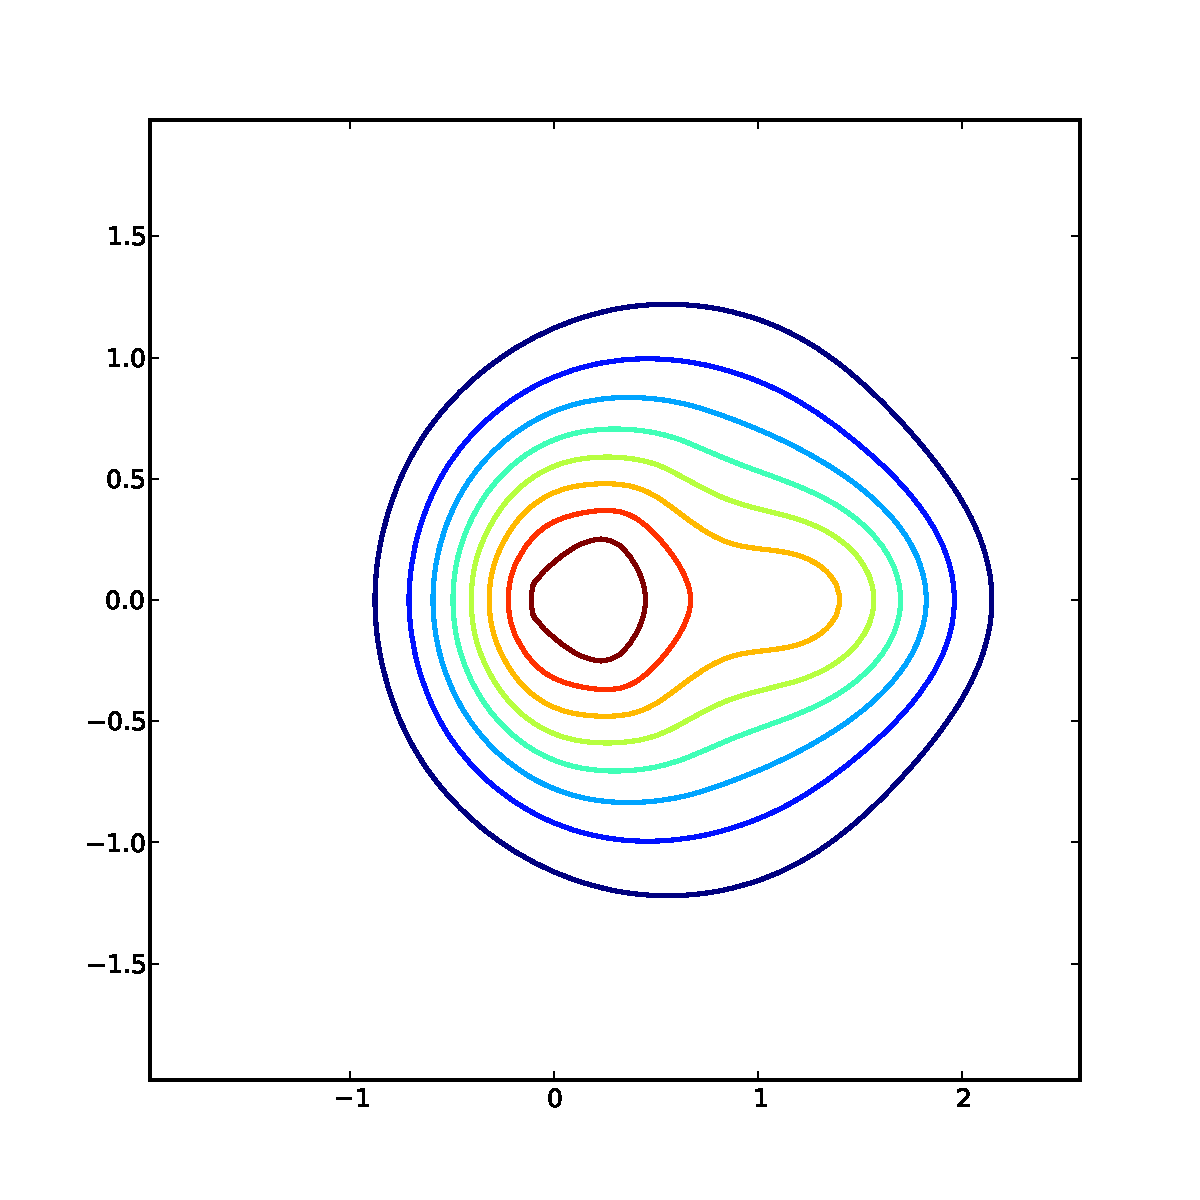
\includegraphics[width=4.2cm]{figs/polboltz/comp2-b2-i2}
}
\caption{Nonconforming experiment with $K=44$, $L=26$.  The times shown are, from left to right,
$t=0,\,0.5,\,1.0$. See Section~\vref{sec:nonconf} for details.}
\label{fig:numpol-nc}
\end{figure}

\begin{figure}
    \centering
    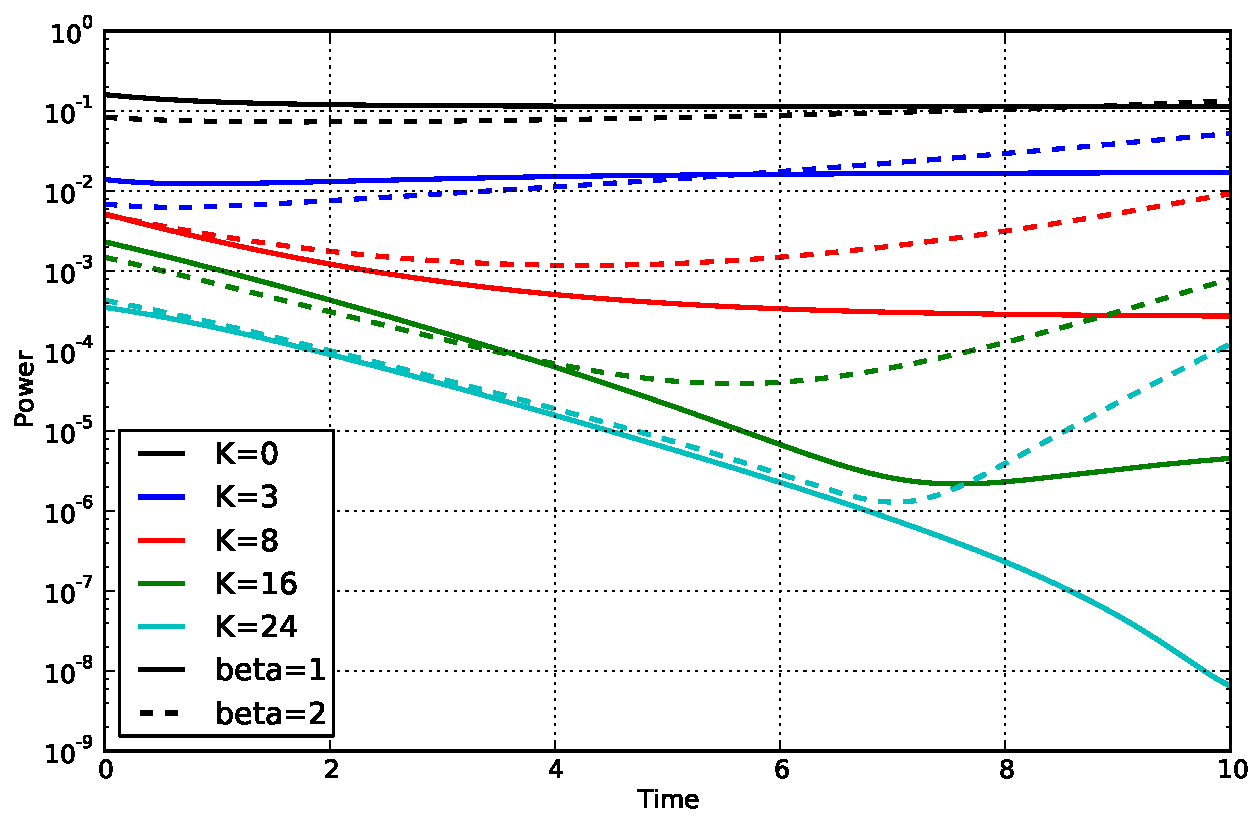
\includegraphics[width=12cm]{figs/polboltz/power-comp2}
    \caption{Power contribution for some values of $k$ for the nonconforming experiment. See
    Section~\vref{sec:nonconf} for details.}
    \label{fig:numpol-nc-power}
\end{figure}

\begin{figure}
\centering
\subfloat[$\beta=1$]{
    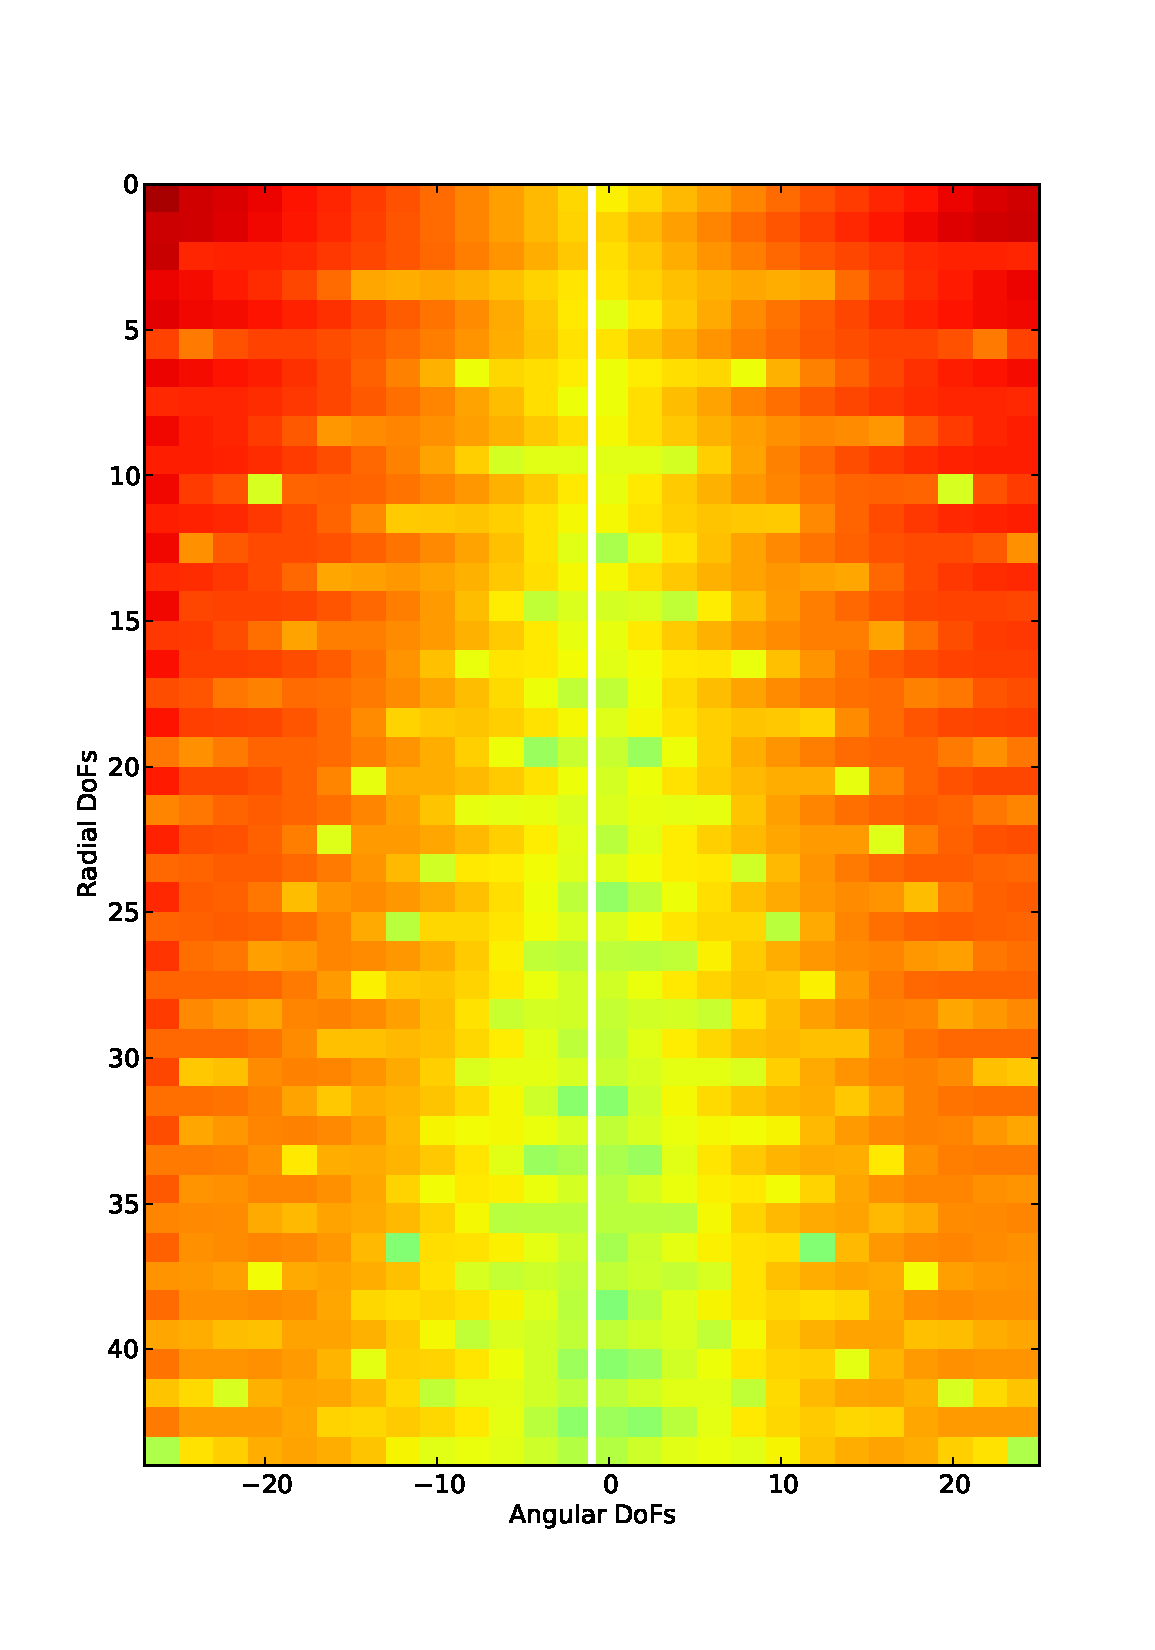
\includegraphics[width=4.2cm]{figs/polboltz/comp2-spec-b1-i0}
    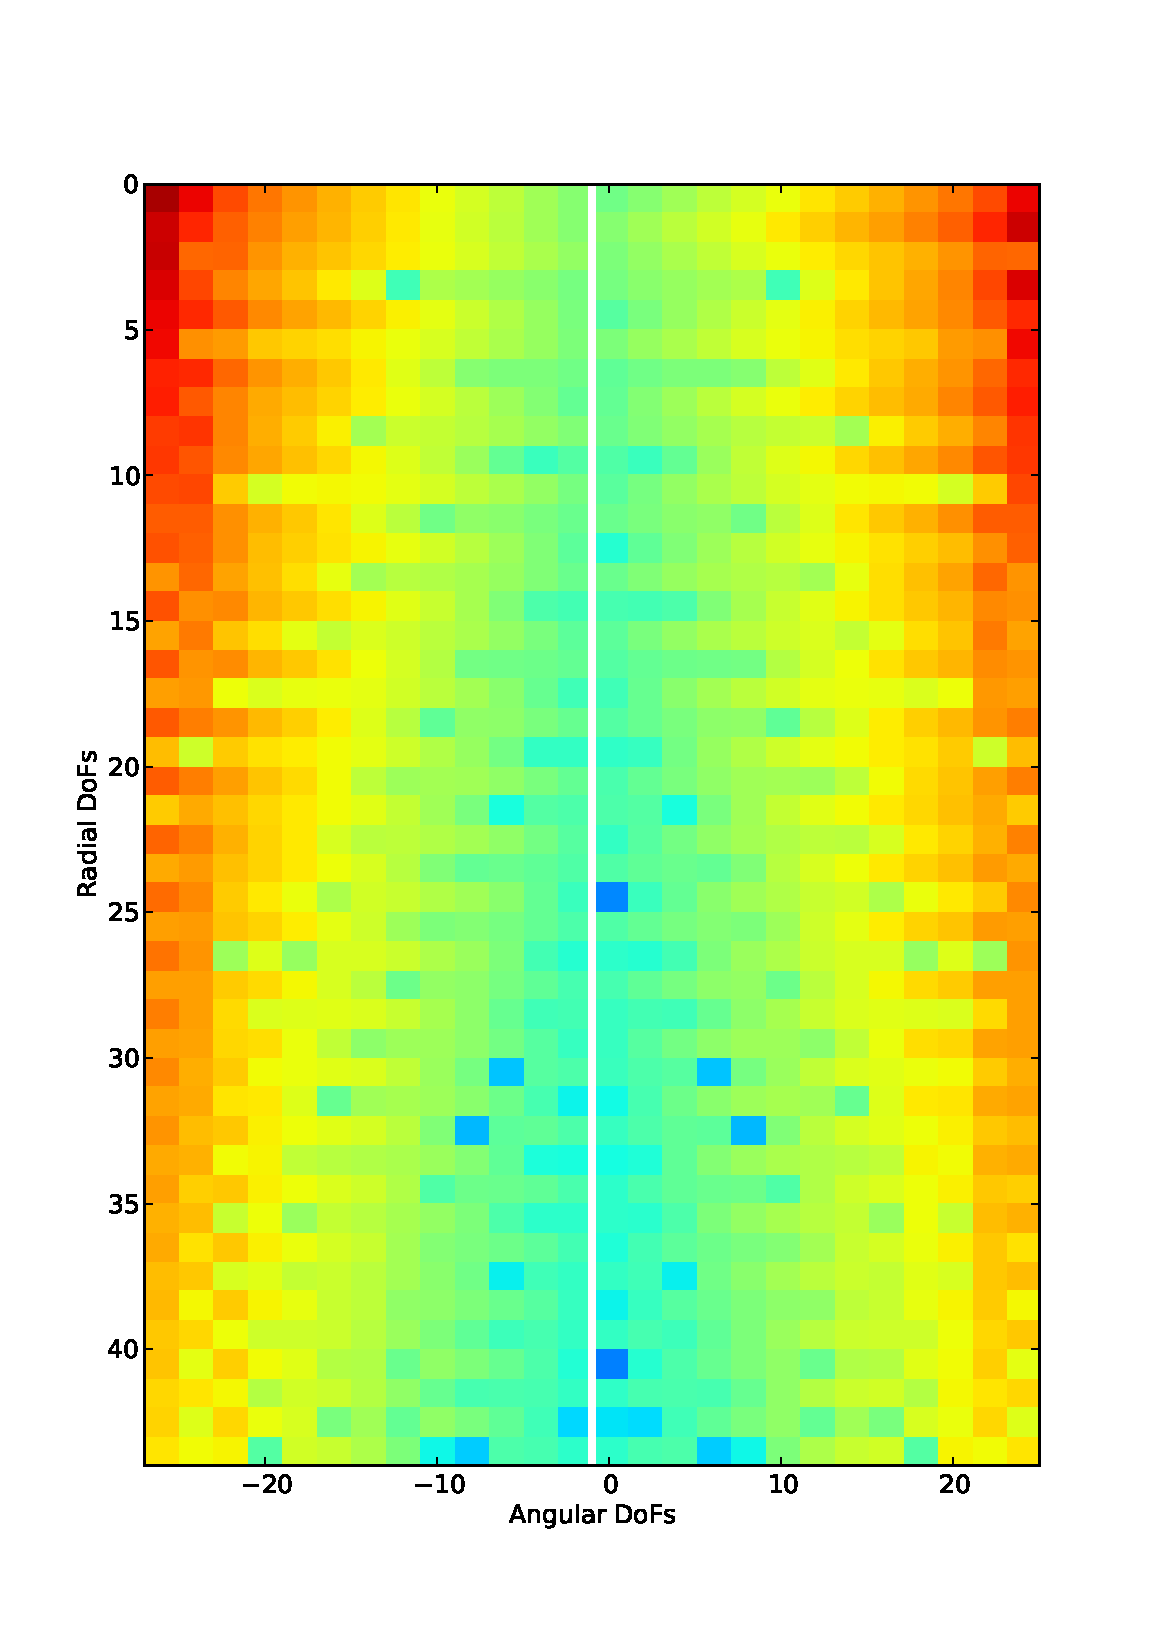
\includegraphics[width=4.2cm]{figs/polboltz/comp2-spec-b1-i2}
    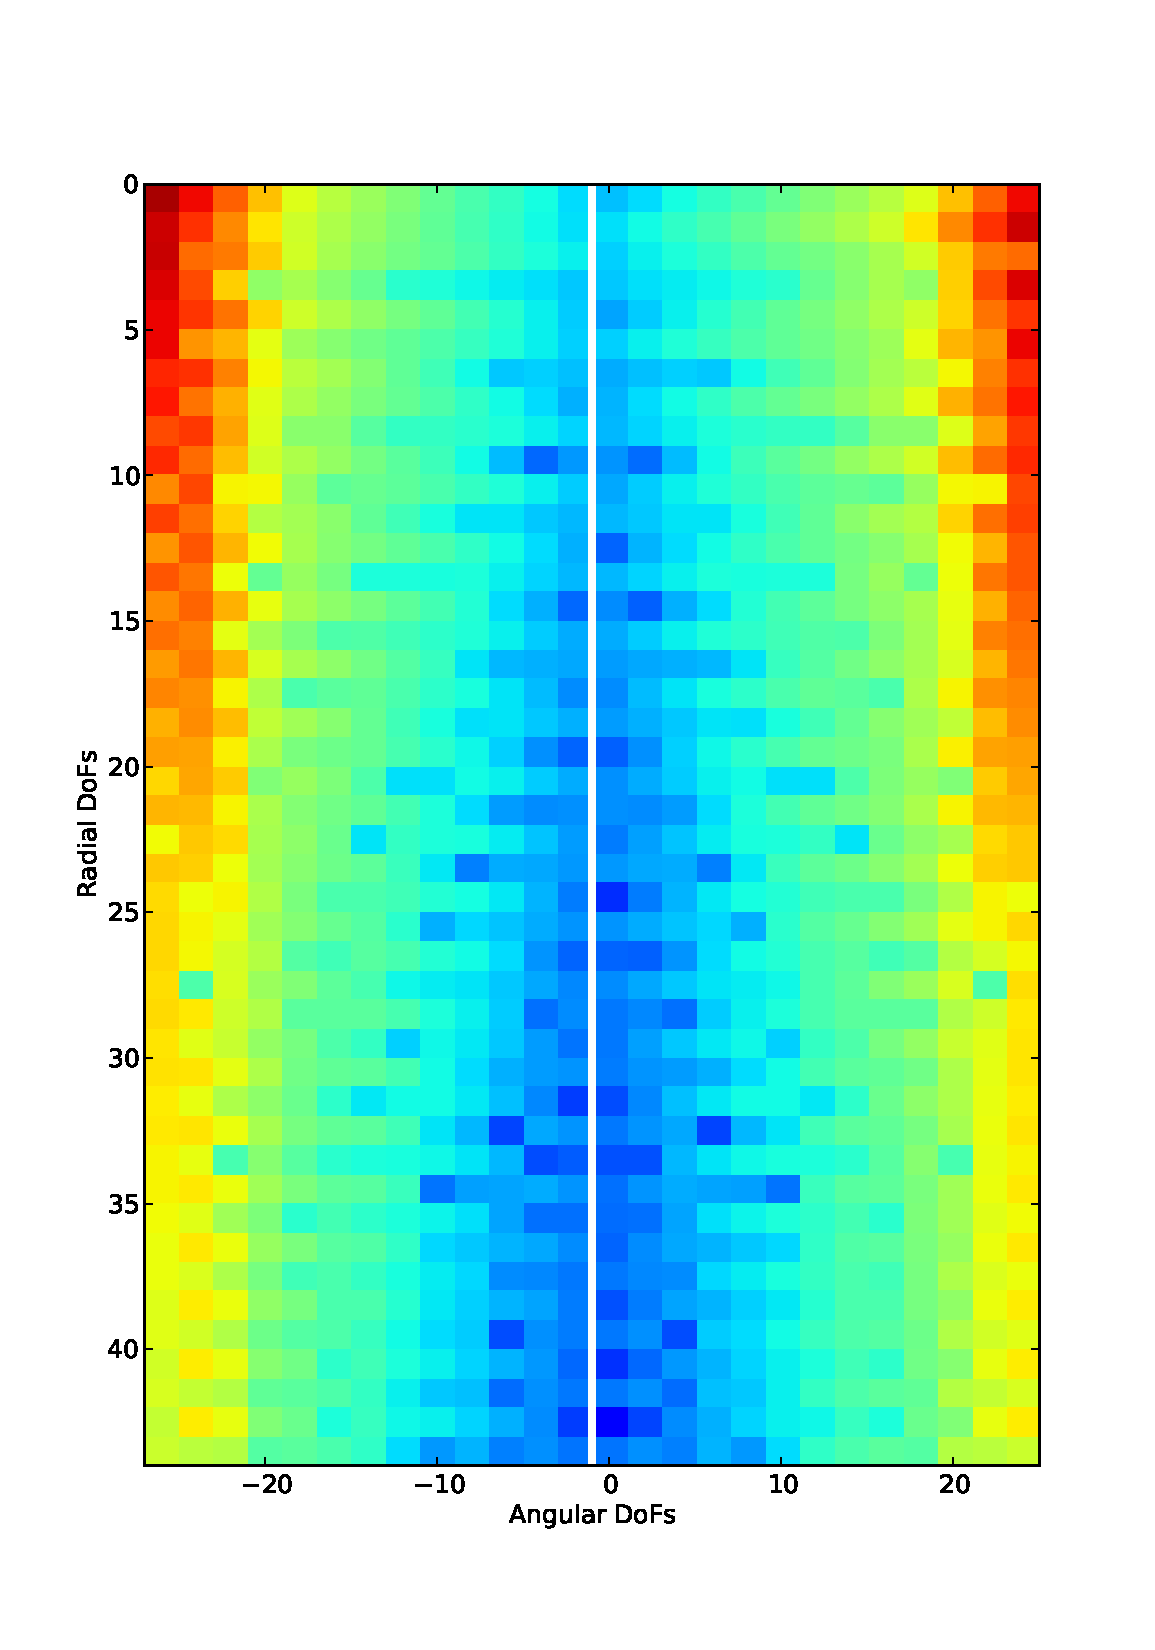
\includegraphics[width=4.2cm]{figs/polboltz/comp2-spec-b1-i3}
} \\
\subfloat[$\beta=2$]{
    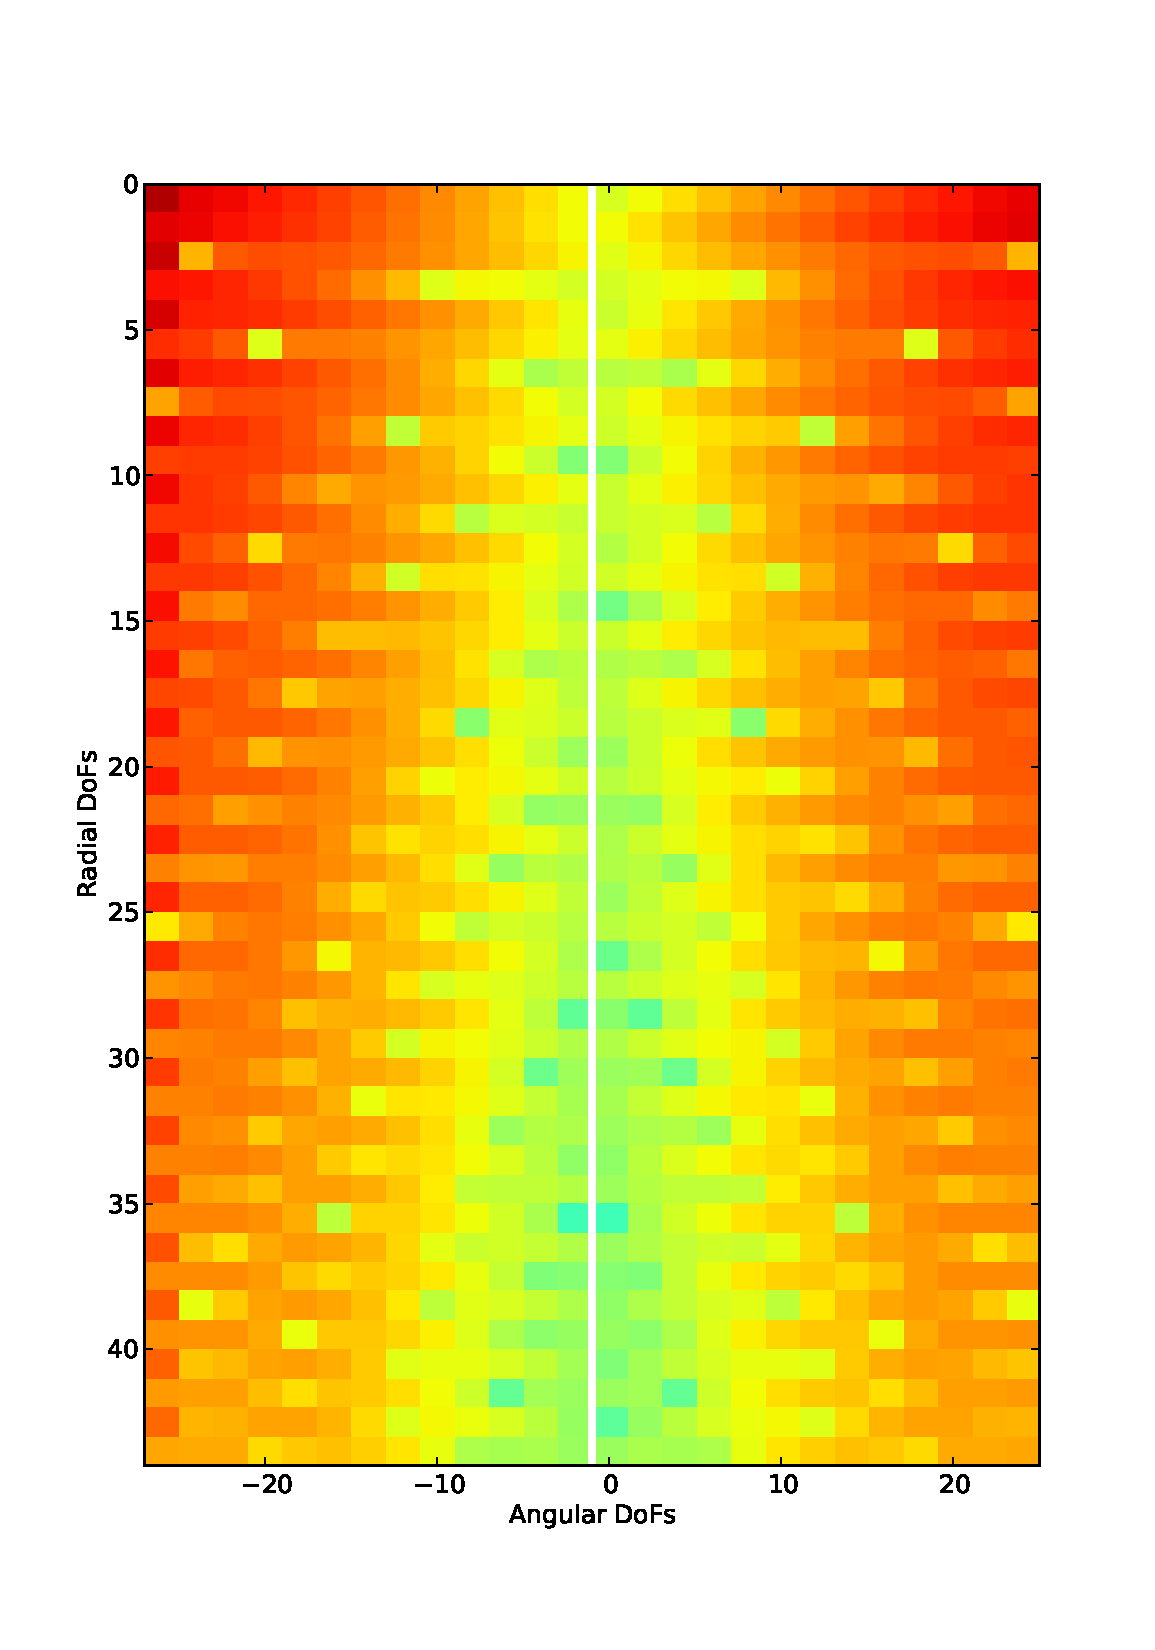
\includegraphics[width=4.2cm]{figs/polboltz/comp2-spec-b2-i0}
    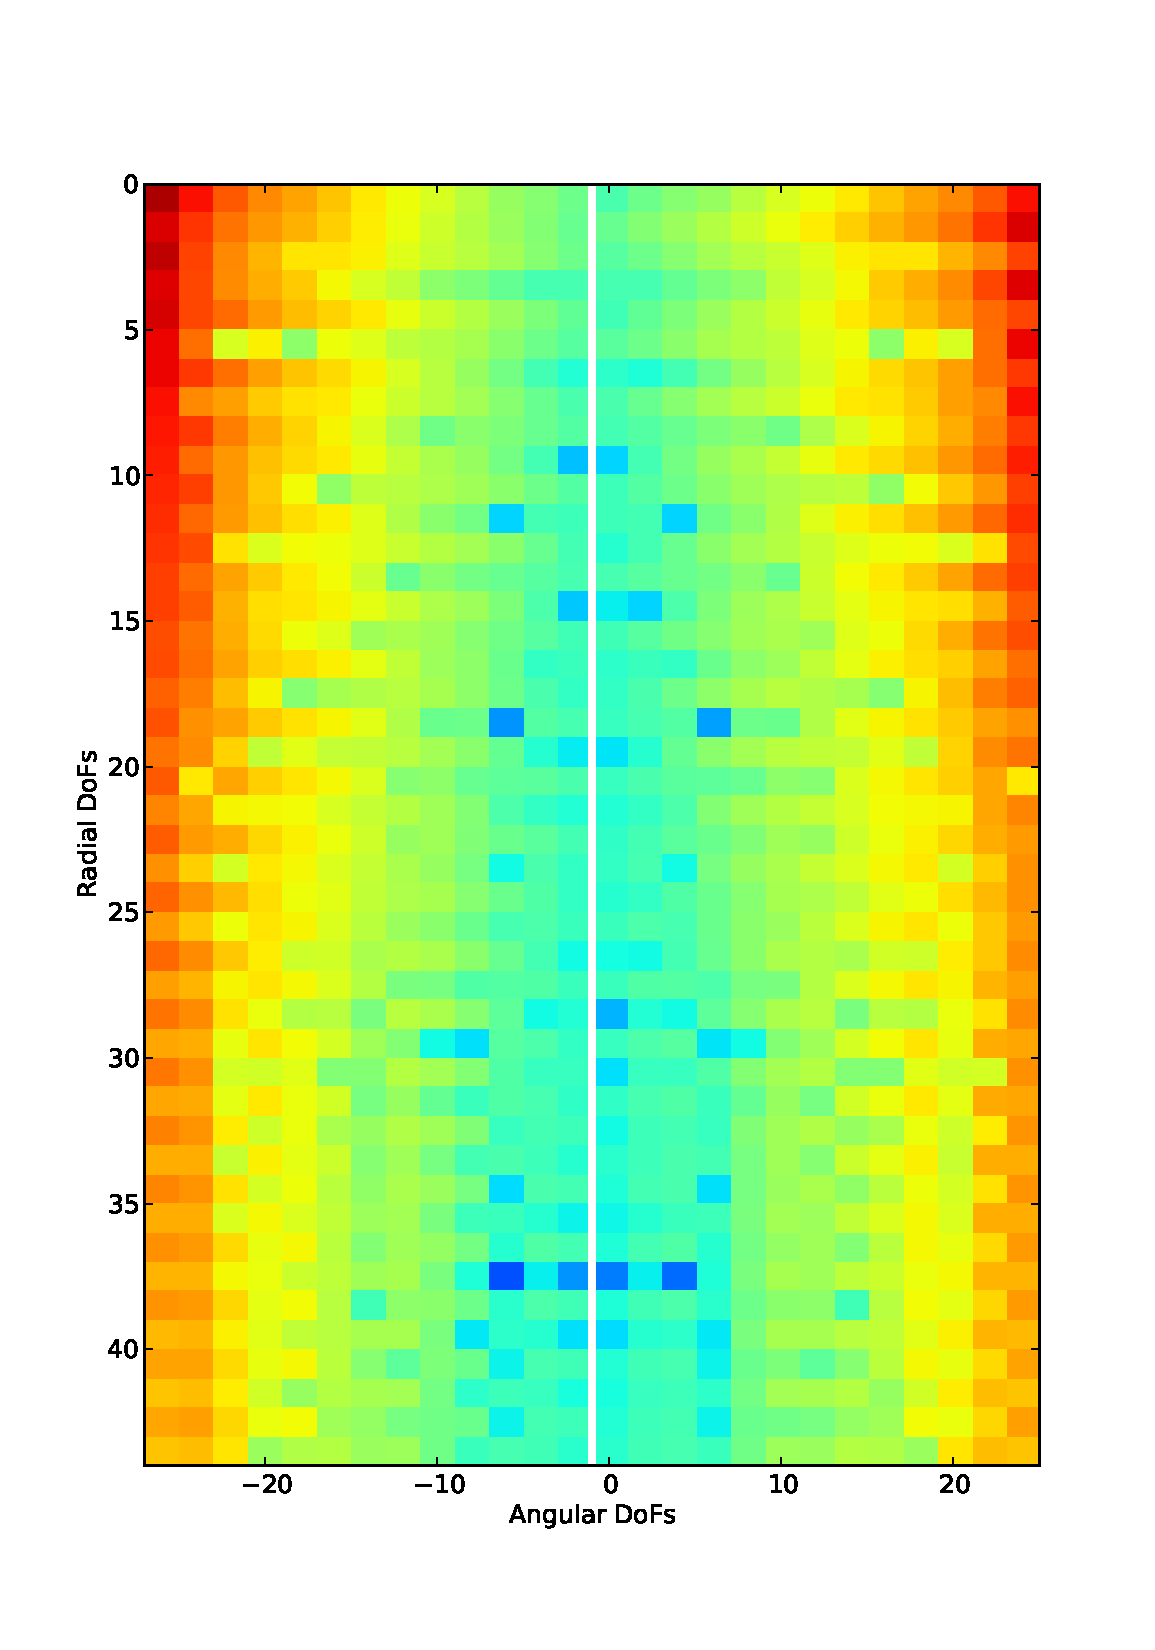
\includegraphics[width=4.2cm]{figs/polboltz/comp2-spec-b2-i2}
    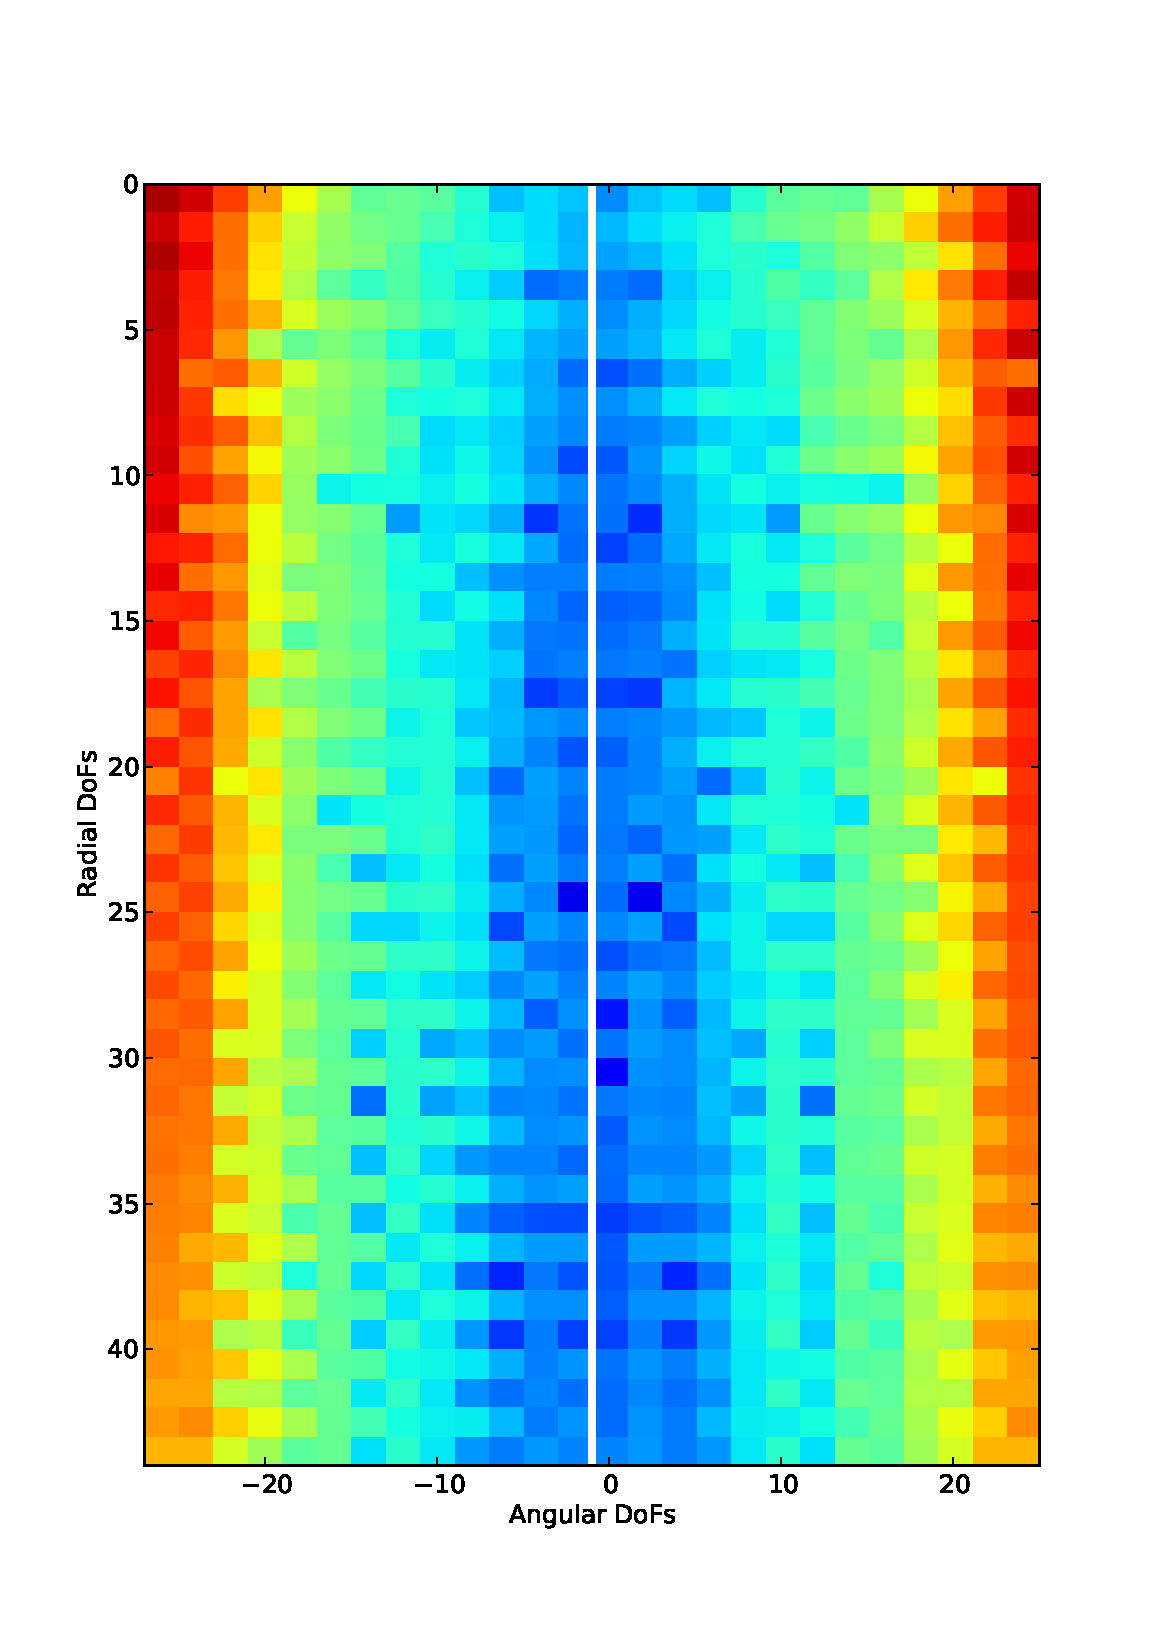
\includegraphics[width=4.2cm]{figs/polboltz/comp2-spec-b2-i3}
}
\caption{Spectral magnitudes for the nonconforming experiment.  The times shown are, from left to right,
$t=0,\,5,\,10$. No shrinkage of the solution space was achieved here with a strict threshold value of
$10^{-10}$. Compare to Figure~\ref{fig:numpol-cb-spec}. See Section~\vref{sec:nonconf} for details.}
\label{fig:numpol-nc-spec}
\end{figure}

\clearpage

\section{Comparison with Fourier discretization}
\label{sec:numerical-fou-pol}

We offer here some concluding remarks on the viability of the two methods presented.

With $N^2$ degrees of freedom, the Fourier discretization can perform a timestep in $\cO(N^4)$ time, and with
$KL$ degrees of freedom, the Polar discretization uses $\cO(K^3 L^2)$ time per timestep. In addition to this,
the convergence in radial direction is only $\cO(\ee^{-\sqrt{K}})$ compared to $\cO(\ee^{-N})$ in all
directions for the Fourier discretization, assuming an analytic solution. Both methods require a one-time
setup where the discrete collision operator is computed, but this step depends only on the kernel.

With this in mind, it seems unlikely that the Polar discretization can outperform the Fourier method. It can
be argued that the Polar method will yield more physical solutions (especially for $\beta=1$), as it is both
fully conservative and devoid of aliasing effects. The Polar method also performs exceptionally well with
near-equilibrium solutions, while the Fourier method has constant performance across the board (or possibly,
as the case may be for the hyperbolic cross method, it performs well for some solutions that are far removed
from equilibrium).

It has proven challenging to directly compare the error performance of the two methods in a realistic
experiment. Since the only known exact solution to \eqref{eqn:boltzmann-sphom} is the isotropic BKW solution
(which gives the Polar method an unfair advantage), we have to resort to reference solutions computed with
very high accuracy. For this, we have again used the crossed streams solution of Section~\vref{sec:numpol-cb}.

Reference solutions were computed using the full Fourier method (with $100\times100=10^4$ degrees of freedom),
and with the Polar method (with $44\times26=1144$ degrees of freedom). The comparison solutions were computed
for the Fourier method on $N\times N$-grids for $N=8,10,12,14$, and for the Polar method on
$N\times\nicefrac{N}{2}$-grids for $N=12,16,20$. These numbers give comparable total numbers of degrees of
freedom ($[64,196]$ for Fourier and $[72,200]$ for Polar).

\begin{figure}
\centering
\subfloat[Reference solution computed with the Fourier method.]{
    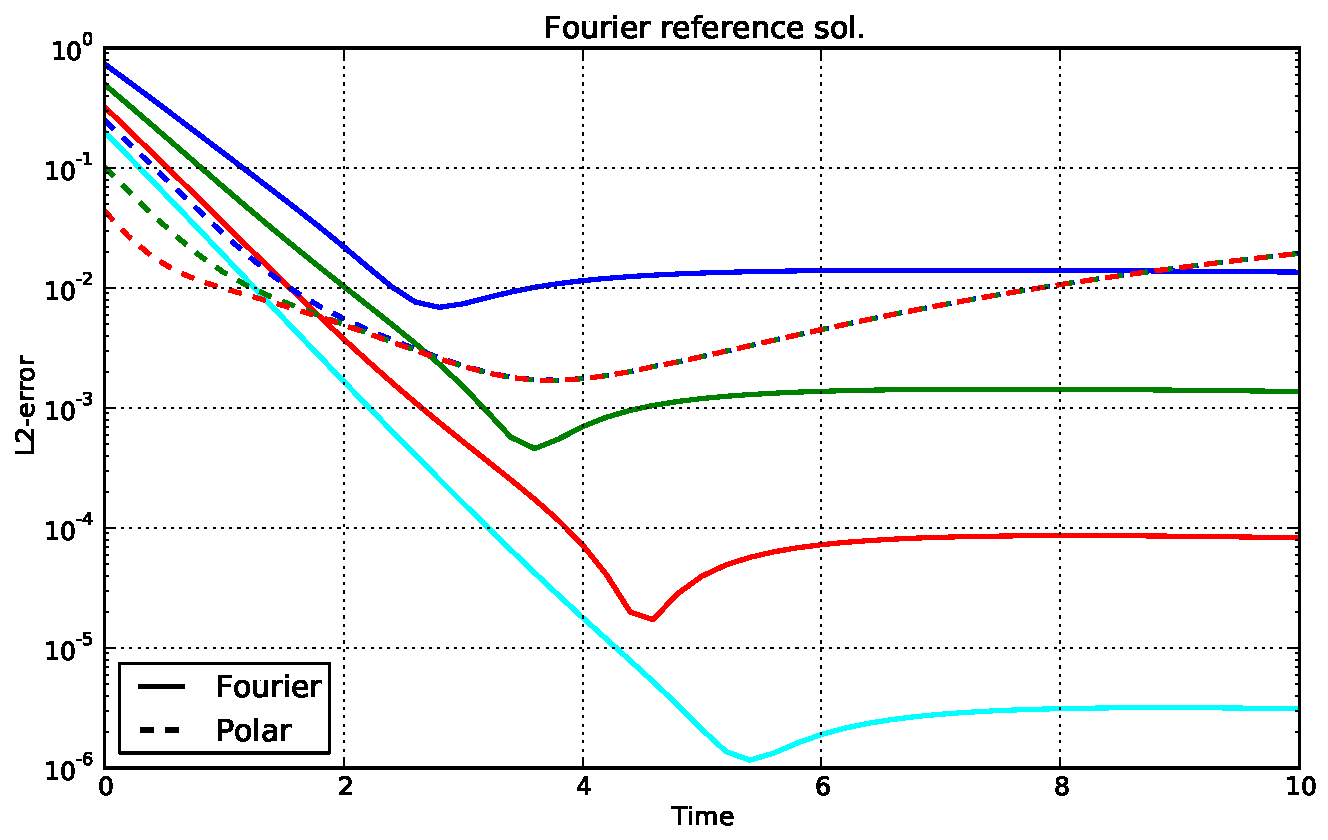
\includegraphics[width=10cm]{figs/polboltz/compare-fourier}} \\
\subfloat[Reference solution computed with the Polar method.]{
    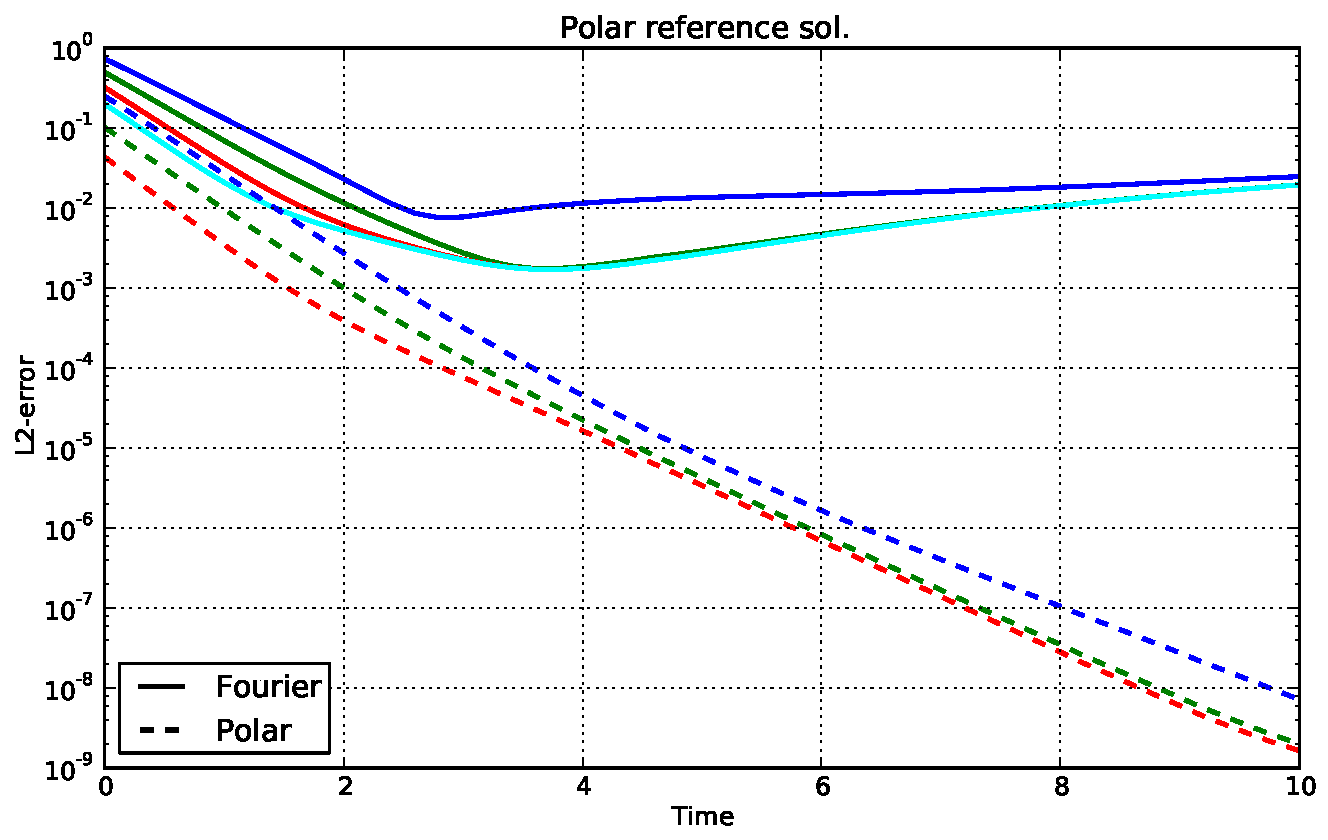
\includegraphics[width=10cm]{figs/polboltz/compare-polar}}
\caption{Comparison using reference solutions computed with the two different methods for the crossed streams
experiment. Note the $y$-axis scales. See Section~\vref{sec:numerical-fou-pol} for details.}
\label{fig:numpol-compare}
\end{figure}

\begin{figure}
    \centering
    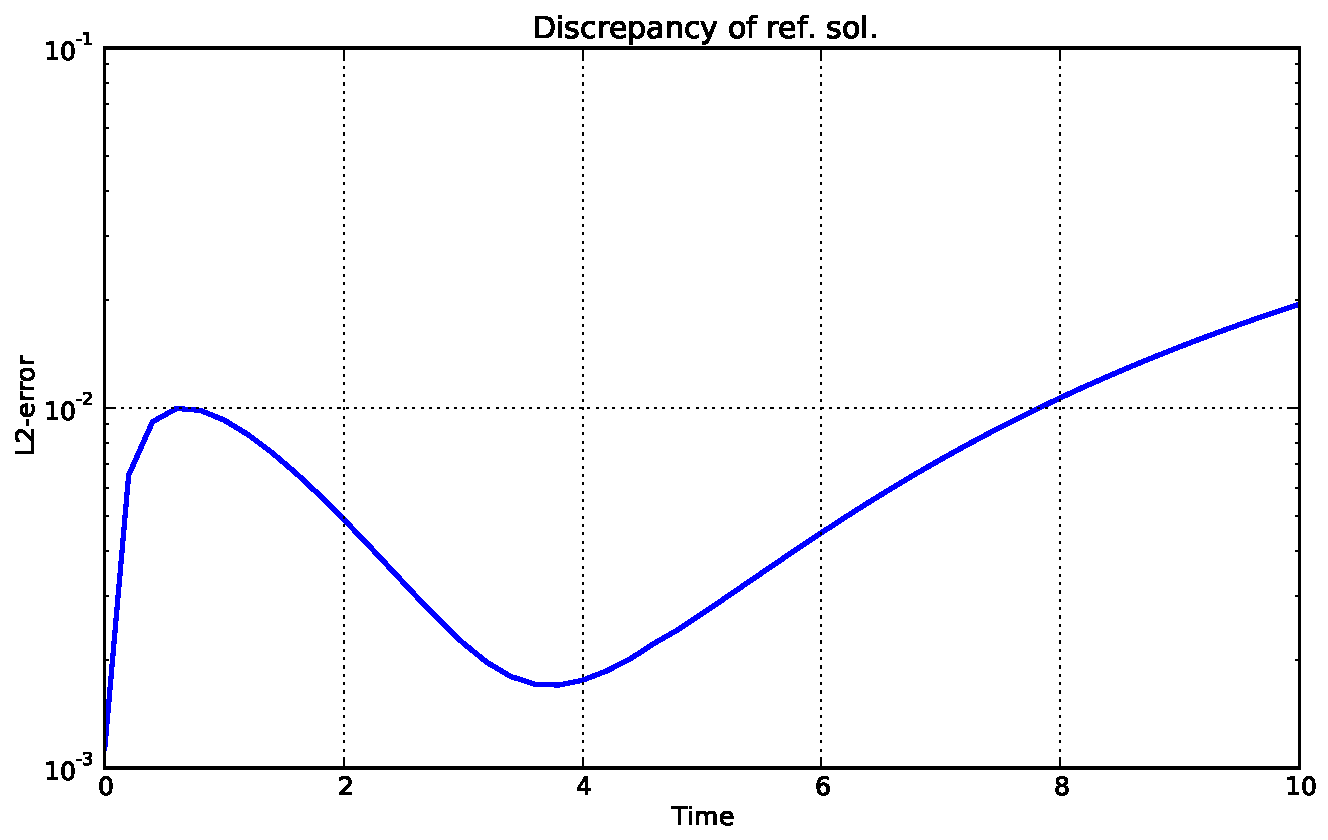
\includegraphics[width=10cm]{figs/polboltz/compare-both}
    \caption{The discrepancy between the two reference solutions from the crossed streams experiment of
    Figure~\ref{fig:numpol-compare}, measured in the $L^2$-norm. See Section~\vref{sec:numerical-fou-pol} for
    details.}
    \label{fig:numpol-compare-disc}
\end{figure}

The results of this experiment can be seen in Figure~\ref{fig:numpol-compare}. The cross-method errors
are all dominated by the difference between the two reference solutions, and consistently level off at about
$10^{-2}$ (see Figure~\ref{fig:numpol-compare-disc}). This disagreement between the methods can presumably be
explained by either
\begin{enumerate}
\renewcommand{\labelenumi}{(\roman{enumi})}
\item dissipative effects from explicit timestepping, or
\item aliasing error introduced in the Fourier method (compare Figures~\ref{fig:numpol-compare} and
\ref{fig:testr}).
\end{enumerate}

Attempts to make the reference solutions agree by increasing the period of the Fourier solution (thus limiting
aliasing) was not successful, as the discretization error quickly became dominating instead.

As an additional experiment, we have performed the same analysis on the nonconforming solution of
Section~\ref{sec:nonconf}, while all other values remain the same (grid sizes, etc.), except we have used
$\beta=1$, since from the observations made in Figure~\vref{fig:numpol-cb-power}, the $\beta=2$ method is
may not be reliable for nonconforming (or at least, asymmetrical) solutions. The relevant data can be seen in
Figure~\vref{fig:numpol-comp2}.

Here, the two methods perform comparably well, and the error is {\em not} dominated by the difference between
the reference solutions, but rather by the actual discretization error.

To be able to evaluate more accurately the quality of the two reference solutions we have performed the same
test on the BKW solution, which has a known nontrivial analytic solution. The results are shown in
Figure~\vref{fig:numpol-comp-bkw}, which shows the time-dependent errors for the polar method (with $44$ radial
basis functions), and for three different full-grid Fourier methods with $80\times80$ degrees of freedom,
differing only in the parameter $L$, to attempt to control the aliasing error. The errors were computed only
on the square $[-\pi,\pi]^2$, which is the domain of the smallest Fourier experiment. We observe that the
polar method produces better solutions for the chosen parameters after only a short time.

\begin{figure}
    \centering
    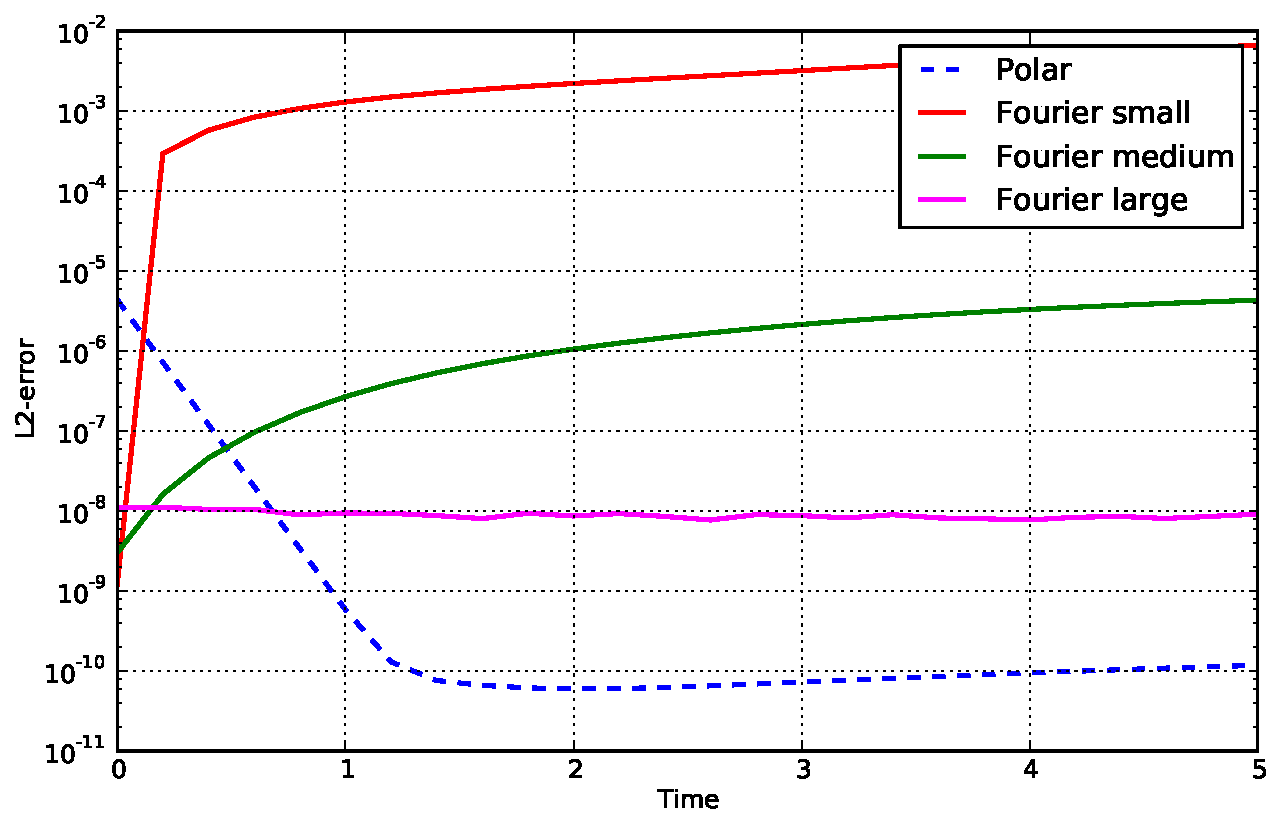
\includegraphics[width=10cm]{figs/polboltz/compare-bkw}
    \caption{Comparison between reference solutions for the BKW solution, defined as $g(\nicefrac{t}{2},
    \sqrt{2}\Bv)$ for $g$ from \eqref{eqn:pol-bkw}. We used $L=\pi, \nicefrac{3\pi}{2}, 3\pi$ for
    the three different Fourier solutions (small, medium and large, respectively) in order to control aliasing
    errors. The Fourier solutions were produced with $80\times80$ degrees of freedom, and the polar solution
    with $44$ radial degrees of freedom. See Section~\vref{sec:numerical-fou-pol} for details.}
    \label{fig:numpol-comp-bkw}
\end{figure}

\begin{figure}
\centering
\subfloat[Reference solution computed with the Fourier method.]{
    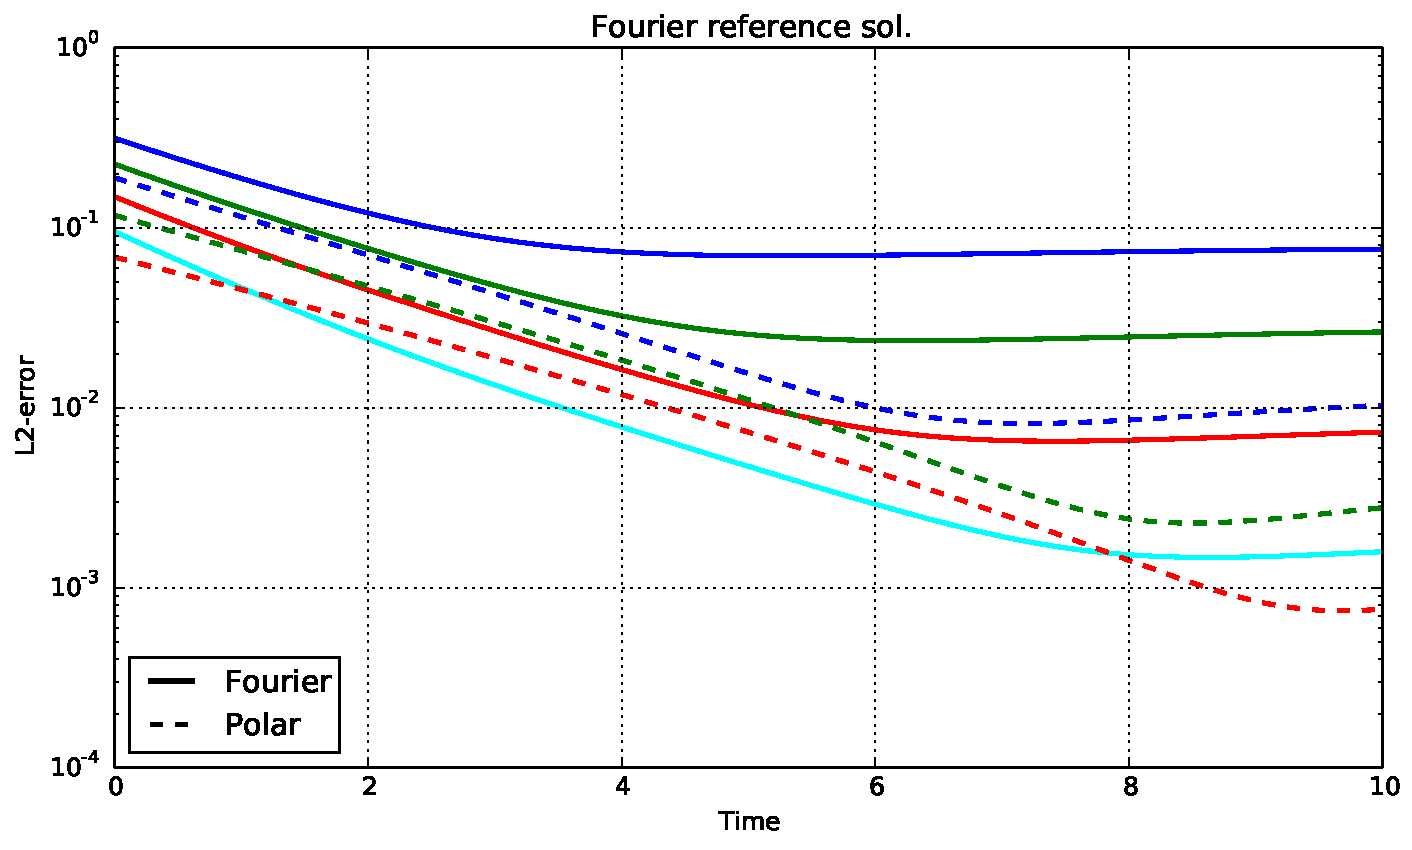
\includegraphics[width=11cm]{figs/polboltz/compare2-fourier}} \\
\subfloat[Reference solution computed with the Polar method.]{
    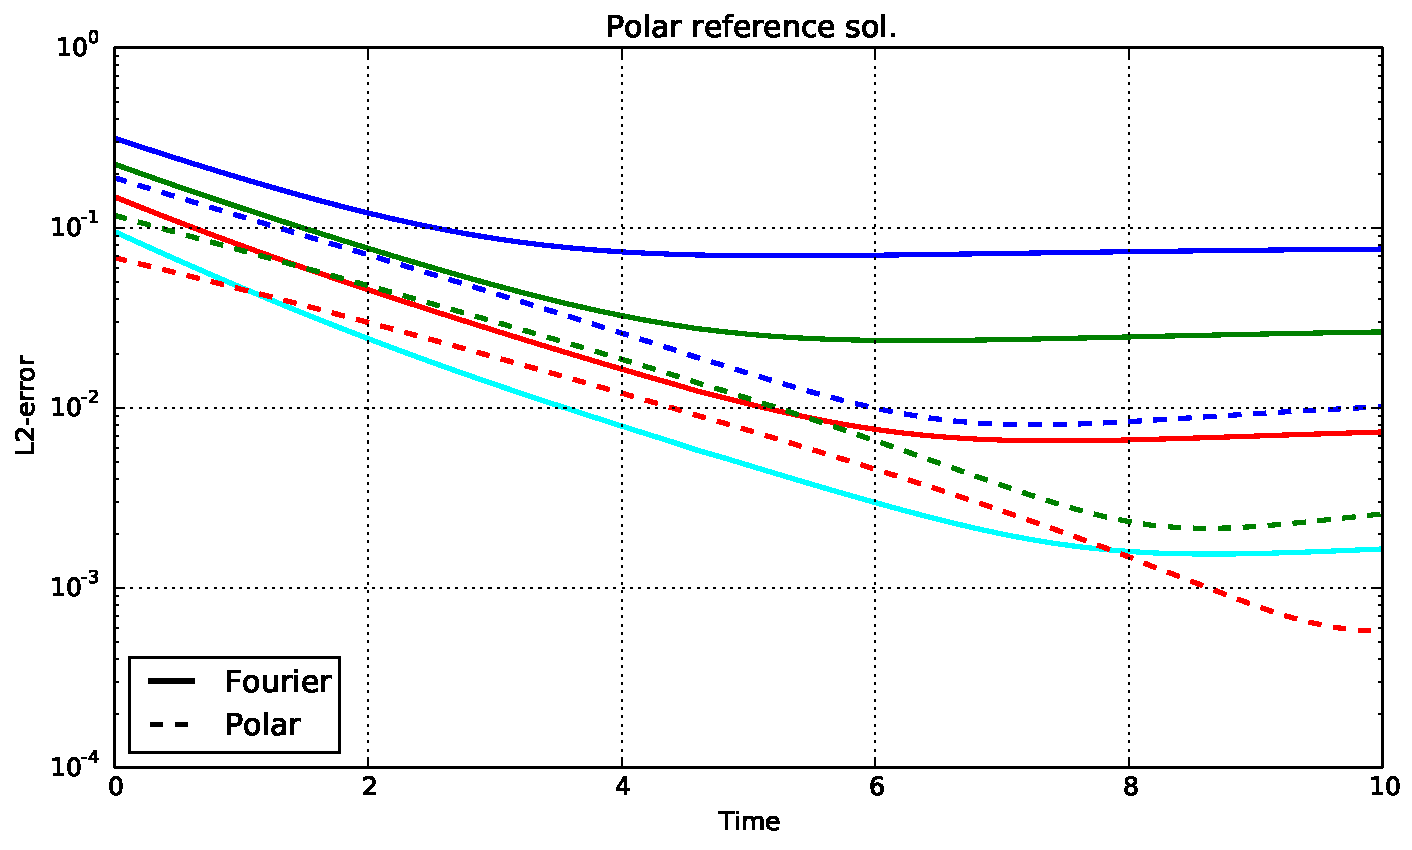
\includegraphics[width=11cm]{figs/polboltz/compare2-polar}}
\caption{Comparison using reference solutions computed with the Fourier method (top) and Polar method (bottom)
for the nonconforming experiment. See Section~\vref{sec:numerical-fou-pol} for details.}
\label{fig:numpol-comp2}
\end{figure}
